\chapter{実験方法}\label{method}
\section{一列配列イオンの捕獲}
\begin{enumerate}
\item まず,$^{40}{\rm Ca}^+$の捕獲に用いるレーザーのセットアップを行う.
\begin{enumerate}
\item 波長計を起動させ,波長計の校正のためにHe-Neレーザーを使用する.
\item 375-nmの電源を点け,電流を65 mAに設定する.
\item 397-nmのmoduleをonにし,CURRENT CTRをonにする.調節ねじを4に回し,電流を51 mA付近に設定する.
\item 866-nm($R_{\rm SET} = 11.682 \ {\rm k}\Omega , I_{0} = 145.16 \ {\rm mA}$)をENABLEに設定する.
\item 423-nmのECDLに電流を60.04 mAを流し,温度を26.550 $^{\circ}$Cに設定する.
\item \Tb{use_laser_wavelength}に$^{40}{\rm Ca}^+$の捕獲を行ったときの波長を示す.なお,$^{40}{\rm Ca}^+$の捕獲に使用する波長はNISTのAtomic Spectra Database Lines Form\cite{NIST}を参照した.

\begin{table}[h]
	\centering
		\caption{$^{40}{\rm Ca}^+$捕獲時に使用するレーザーの波長}
		\label{tab:use_laser_wavelength}
		\begin{tabular}{c}\hline \hline
			632.99050 nm \\
			866.45120 nm \\
			396.95890 nm \\
			422.79157 nm \\ \hline
		\end{tabular}
\end{table}

\item プレーナートラップ上のイオン捕獲位置でレーザーの焦点が合うように真空チャンバーの手前にレンズを設置しており,マイクロメーターを用いて上下左右に移動させることができる.一列配列イオンでは\Fig{lens_string}で示されるイオンが並ぶ方向に対して垂直に照射するレーザーのマイクロメータの初期値として目盛を鉛直方向に4,水平方向に39とし,斜めに照射するレーザーのマイクロメータの初期目盛は鉛直方向が10,水平方向は0と設定する.

 \begin{figure}[h] 
 	\begin{center}
 		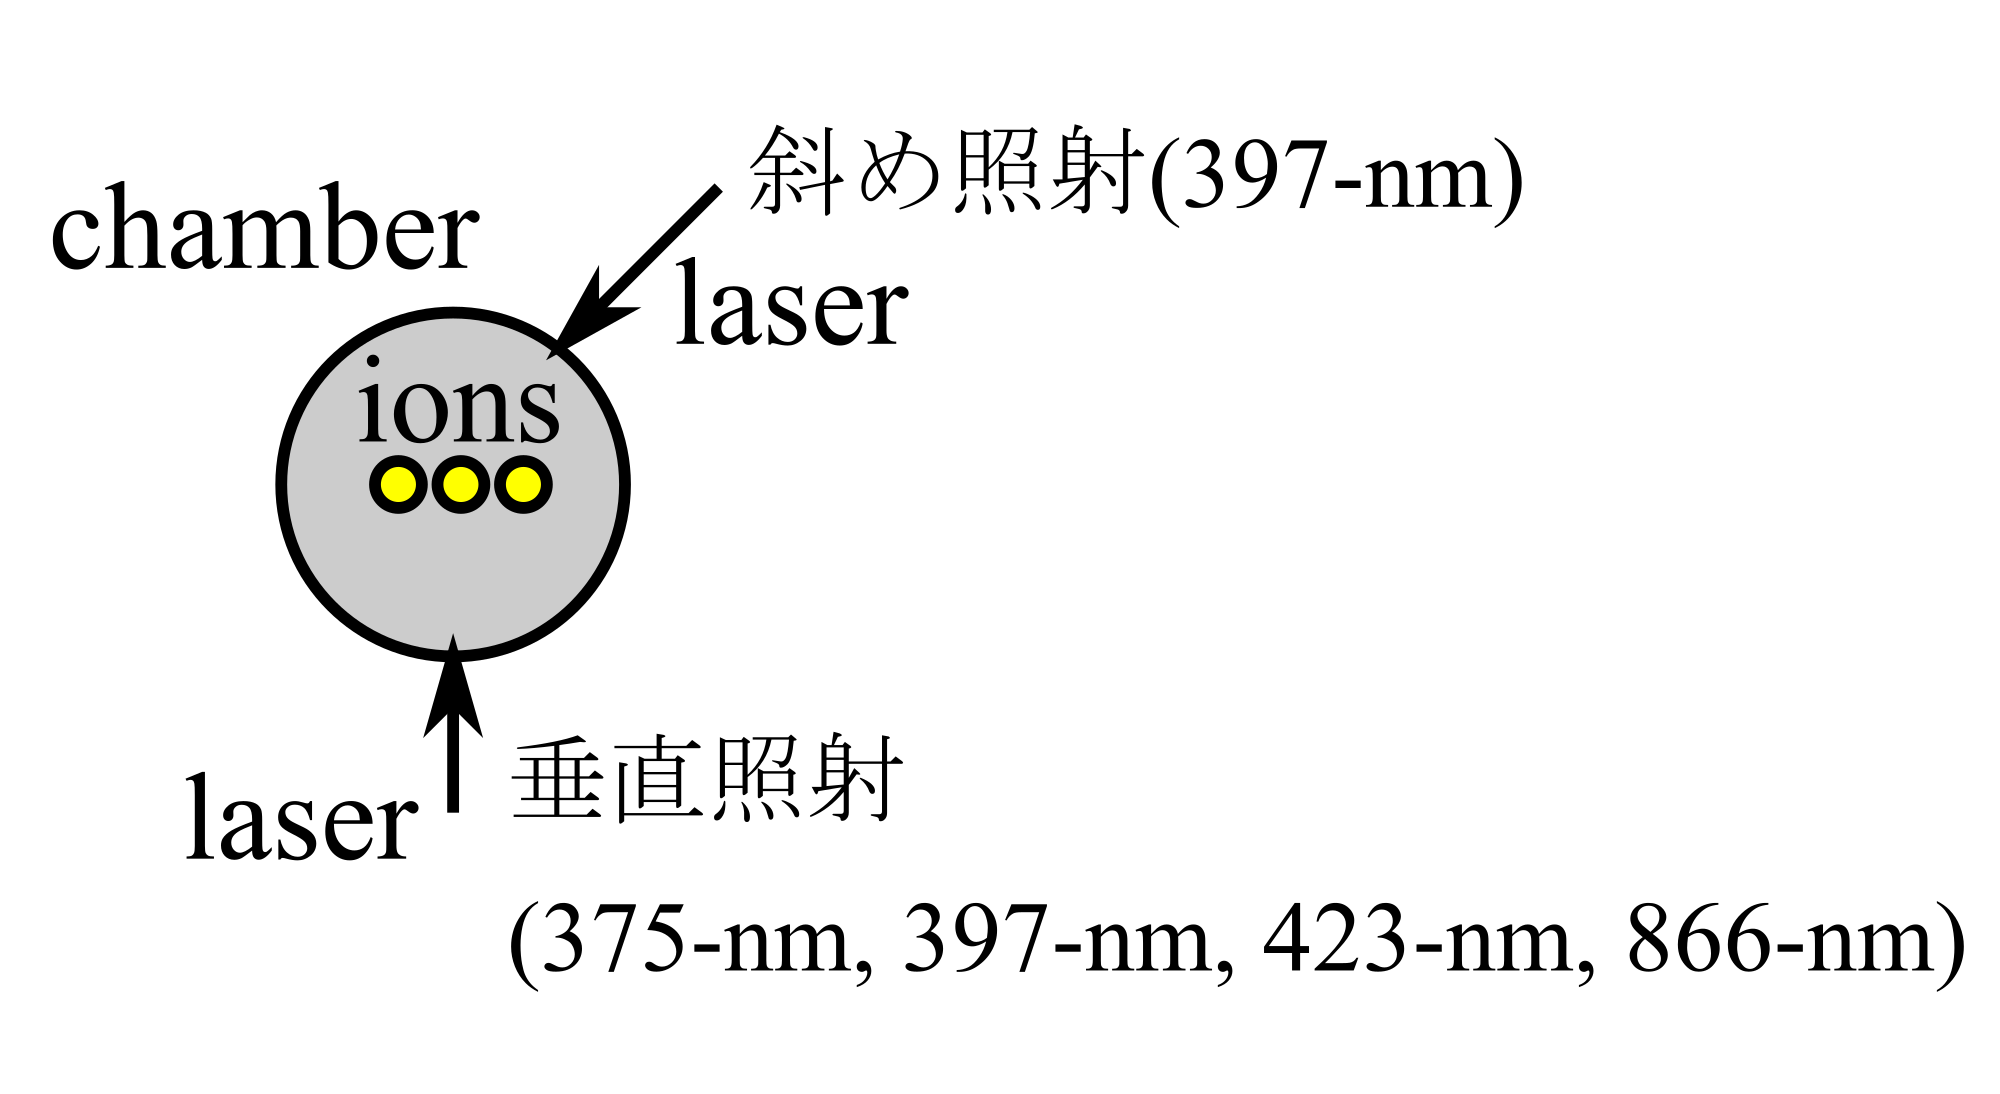
\includegraphics[scale=0.35]{./methods/figure/in_laser.png}
 		\caption{プレーナートラップに照射する二本のレーザー}
 		\label{fig:lens_string}
 	\end{center}
 \end{figure}
\end{enumerate}

\clearpage

\item 次にプレーナートラップに印加するdc電圧とrf電圧のセットアップを行う.
\begin{enumerate}
\item プレーナートラップの各電極に\Tb{dc_string}に示すdc電圧を印加する.

\begin{table}[h]
	\centering
		\caption{一列配列イオンを捕獲するためにプレーナートラップに印加するdc電圧セット}
		\label{tab:dc_string}
		\begin{tabular}{c|r} \hline \hline
			dc電極 & dc電圧 \\ \hline
			End1 & 1.44  V \\
			End2 & 1.406  V \\
			End3 & 1.44  V \\
			End4 & 1.406 V \\
			center & 0.225 V \\
			side1 & 0.222 V \\
			side2 & 0.222 V \\
			middle1 & -1.532 V \\
			middle2 & -1.532 V \\ \hline
		\end{tabular}
\end{table}

\item 発振器を用いてrf信号を発生させる.周波数は27.2 MHzで,rf電極に印加される信号には320 mV$_{\rm pp}$(CH1),center-rf電極に印加される信号には1 mV$_{\rm pp}$(CH2)を設定し,増幅器を利用して,増幅されたrf信号をプレーナートラップに印加する.rf電圧の波形を\Fig{1D_wave}に示す.

\begin{figure}[h]
	\begin{minipage}{0.48\linewidth}
		\begin{center}
			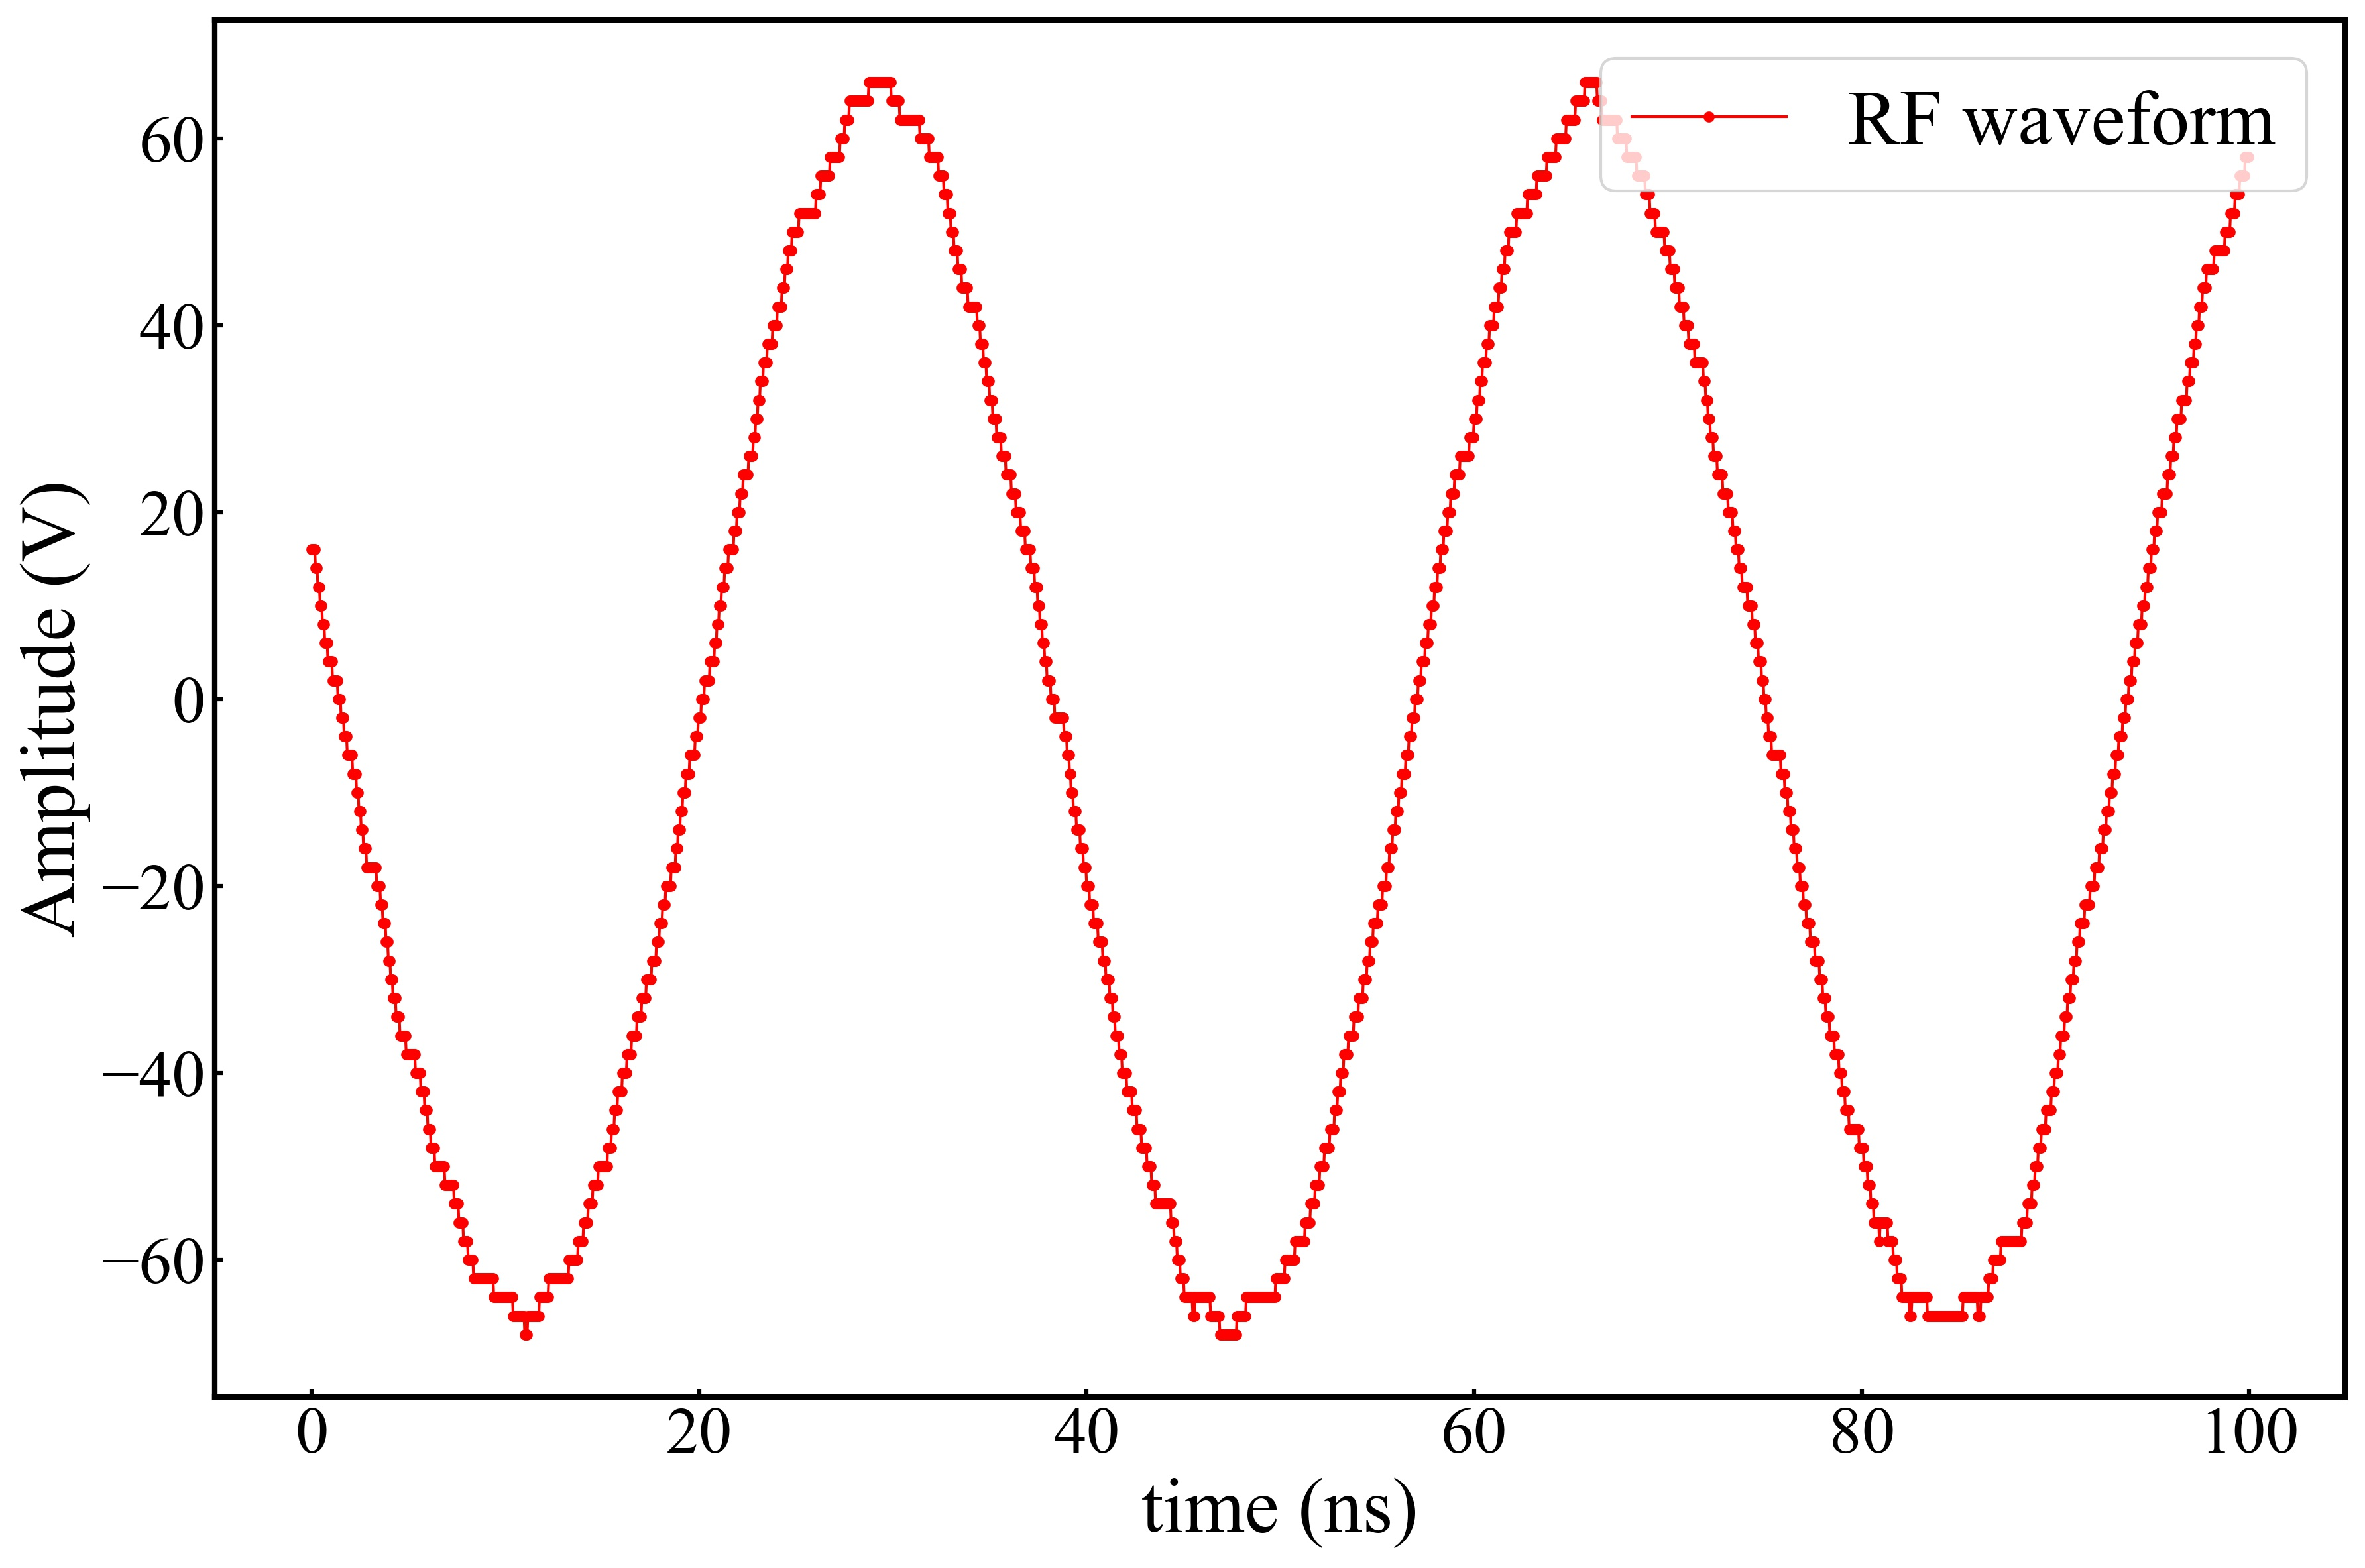
\includegraphics[width=0.9\columnwidth]{./methods/figure/1D_wave.jpg}
			\caption{一列配列イオンを捕獲するために使用するrf電圧の波形}
			\label{fig:1D_wave}
		\end{center}
	\end{minipage}
	\begin{minipage}{0.48\linewidth}
		\begin{center}
			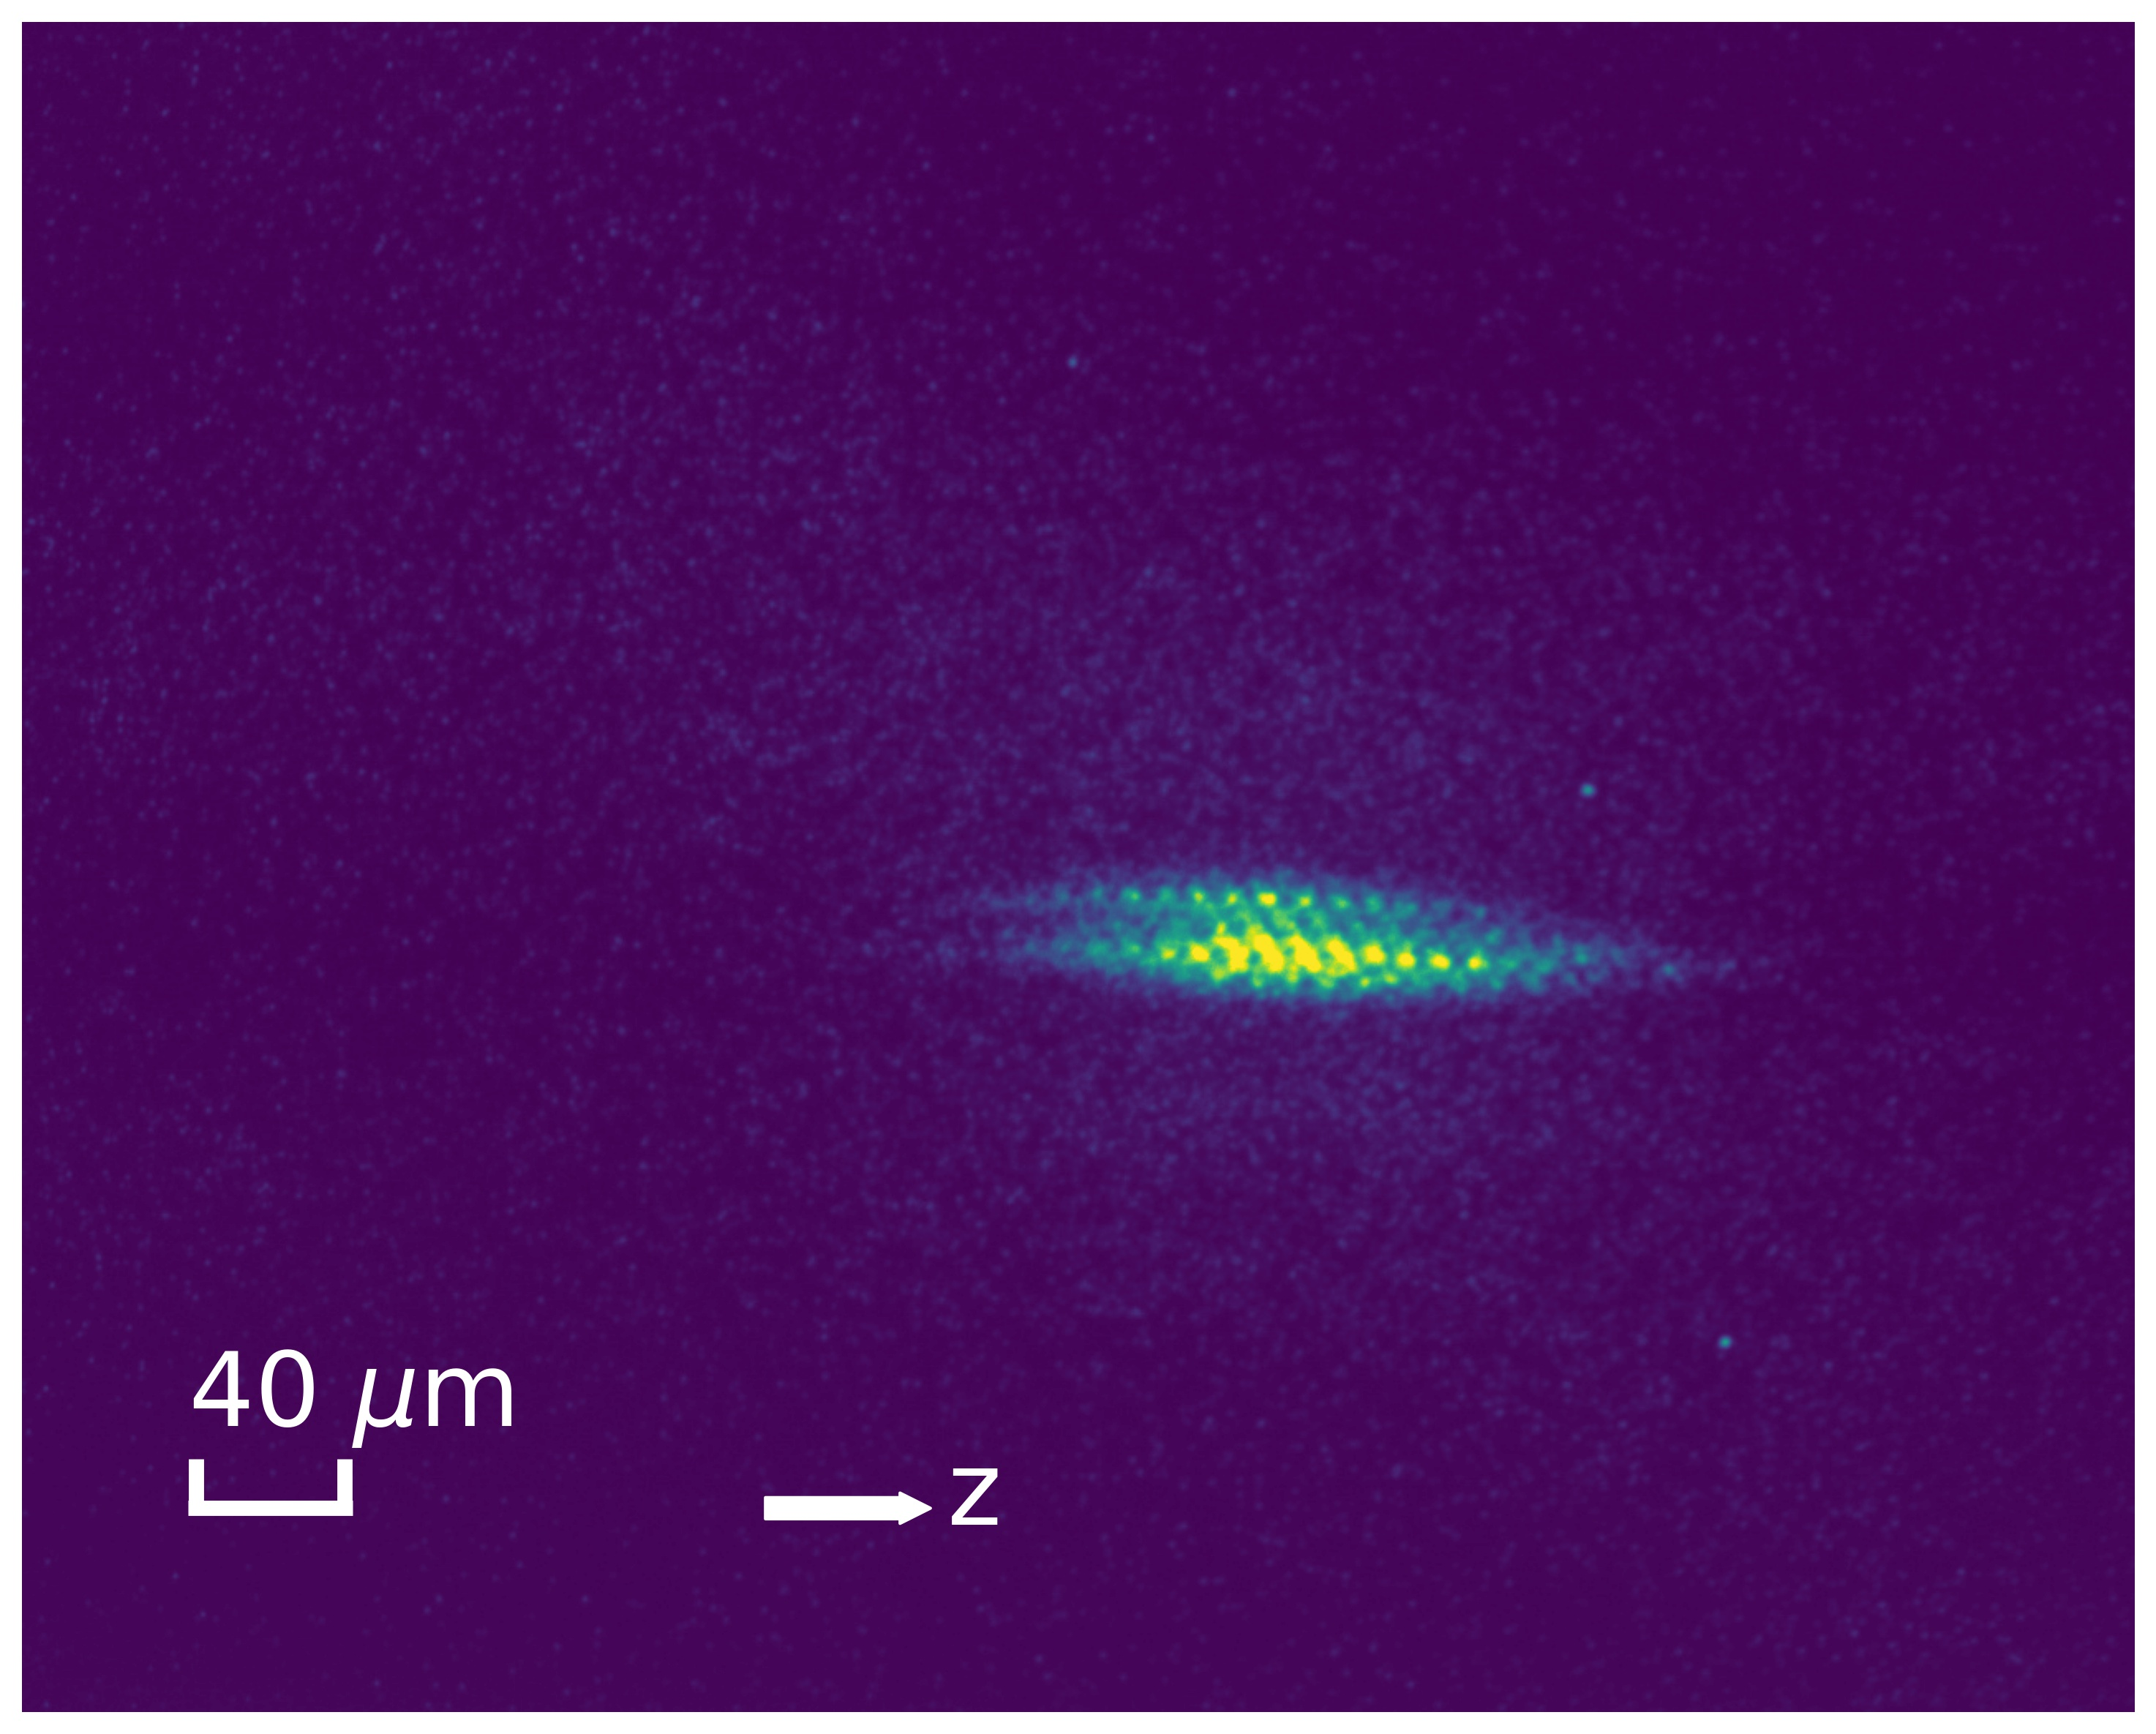
\includegraphics[width=0.6\columnwidth]{./methods/figure/string.jpg}
			\caption{4分間オーブンによる加熱を行ったあとのイオン捕獲画像(真空度 : $2.85 \times 10^{-10}$ Torr)}
			\label{fig:Cap_string}
		\end{center}
	\end{minipage}
\end{figure}

\item 磁場の印加を行い,カルシウム原子を射出させるためにオーブンによる加熱を行う.

\item Image Intensifierと汎用CCDカメラを組み合わせた検出系でイオンの蛍光を集光する.露光時間は10ms,Gainは4.0に設定する.
 
\item オーブンをLabVIEWを介して制御し,適宜レーザーの波長を調節しながらイオンが捕獲されるまでオーブンによる加熱を続ける.

\item 4分間オーブンによる加熱を行ったときのイオン捕獲画像を\Fig{Cap_string}に示している.
\end{enumerate}
\end{enumerate}
%
\clearpage
%
\section{二列配列イオンの捕獲}
二列配列イオンの捕獲手順を説明する.一列配列イオンの捕獲条件との主な変更点は
\begin{itemize}
	\item center-rf信号の振幅
	\item イオン捕獲位置の変化によるレーザー照射位置の調整と集光系のピントの調整
	\item dc電圧の調整
\end{itemize}
の3つである.以下,二列配列イオンの捕獲手順を示す.\\
\begin{enumerate}
\item まずは,一列配列イオンの捕獲条件で多数のイオンの捕獲を行う.\Fig{1_2D}にこのときのイオン捕獲画像,\Fig{1_2D_wave}にオシロスコープで取得したrf電圧とcenter-rf電圧の関係を示す.rf電圧とcenter-rf電圧は発振器で発生させており,発振器上での出力設定はrf電圧の振幅が320 mVpp,位相が0$^{\circ}$,center-rf電圧の振幅が1 mVpp,位相が -40$^{\circ}$となっており,\Fig{1_2D_wave}は発振器から出力されたrf信号を増幅し,プレーナートラップがある真空チャンバーの直前でオシロスコープを用いて計測を行っている.

\begin{figure}[h]
	\begin{minipage}{0.48\linewidth}
	\begin{center}
		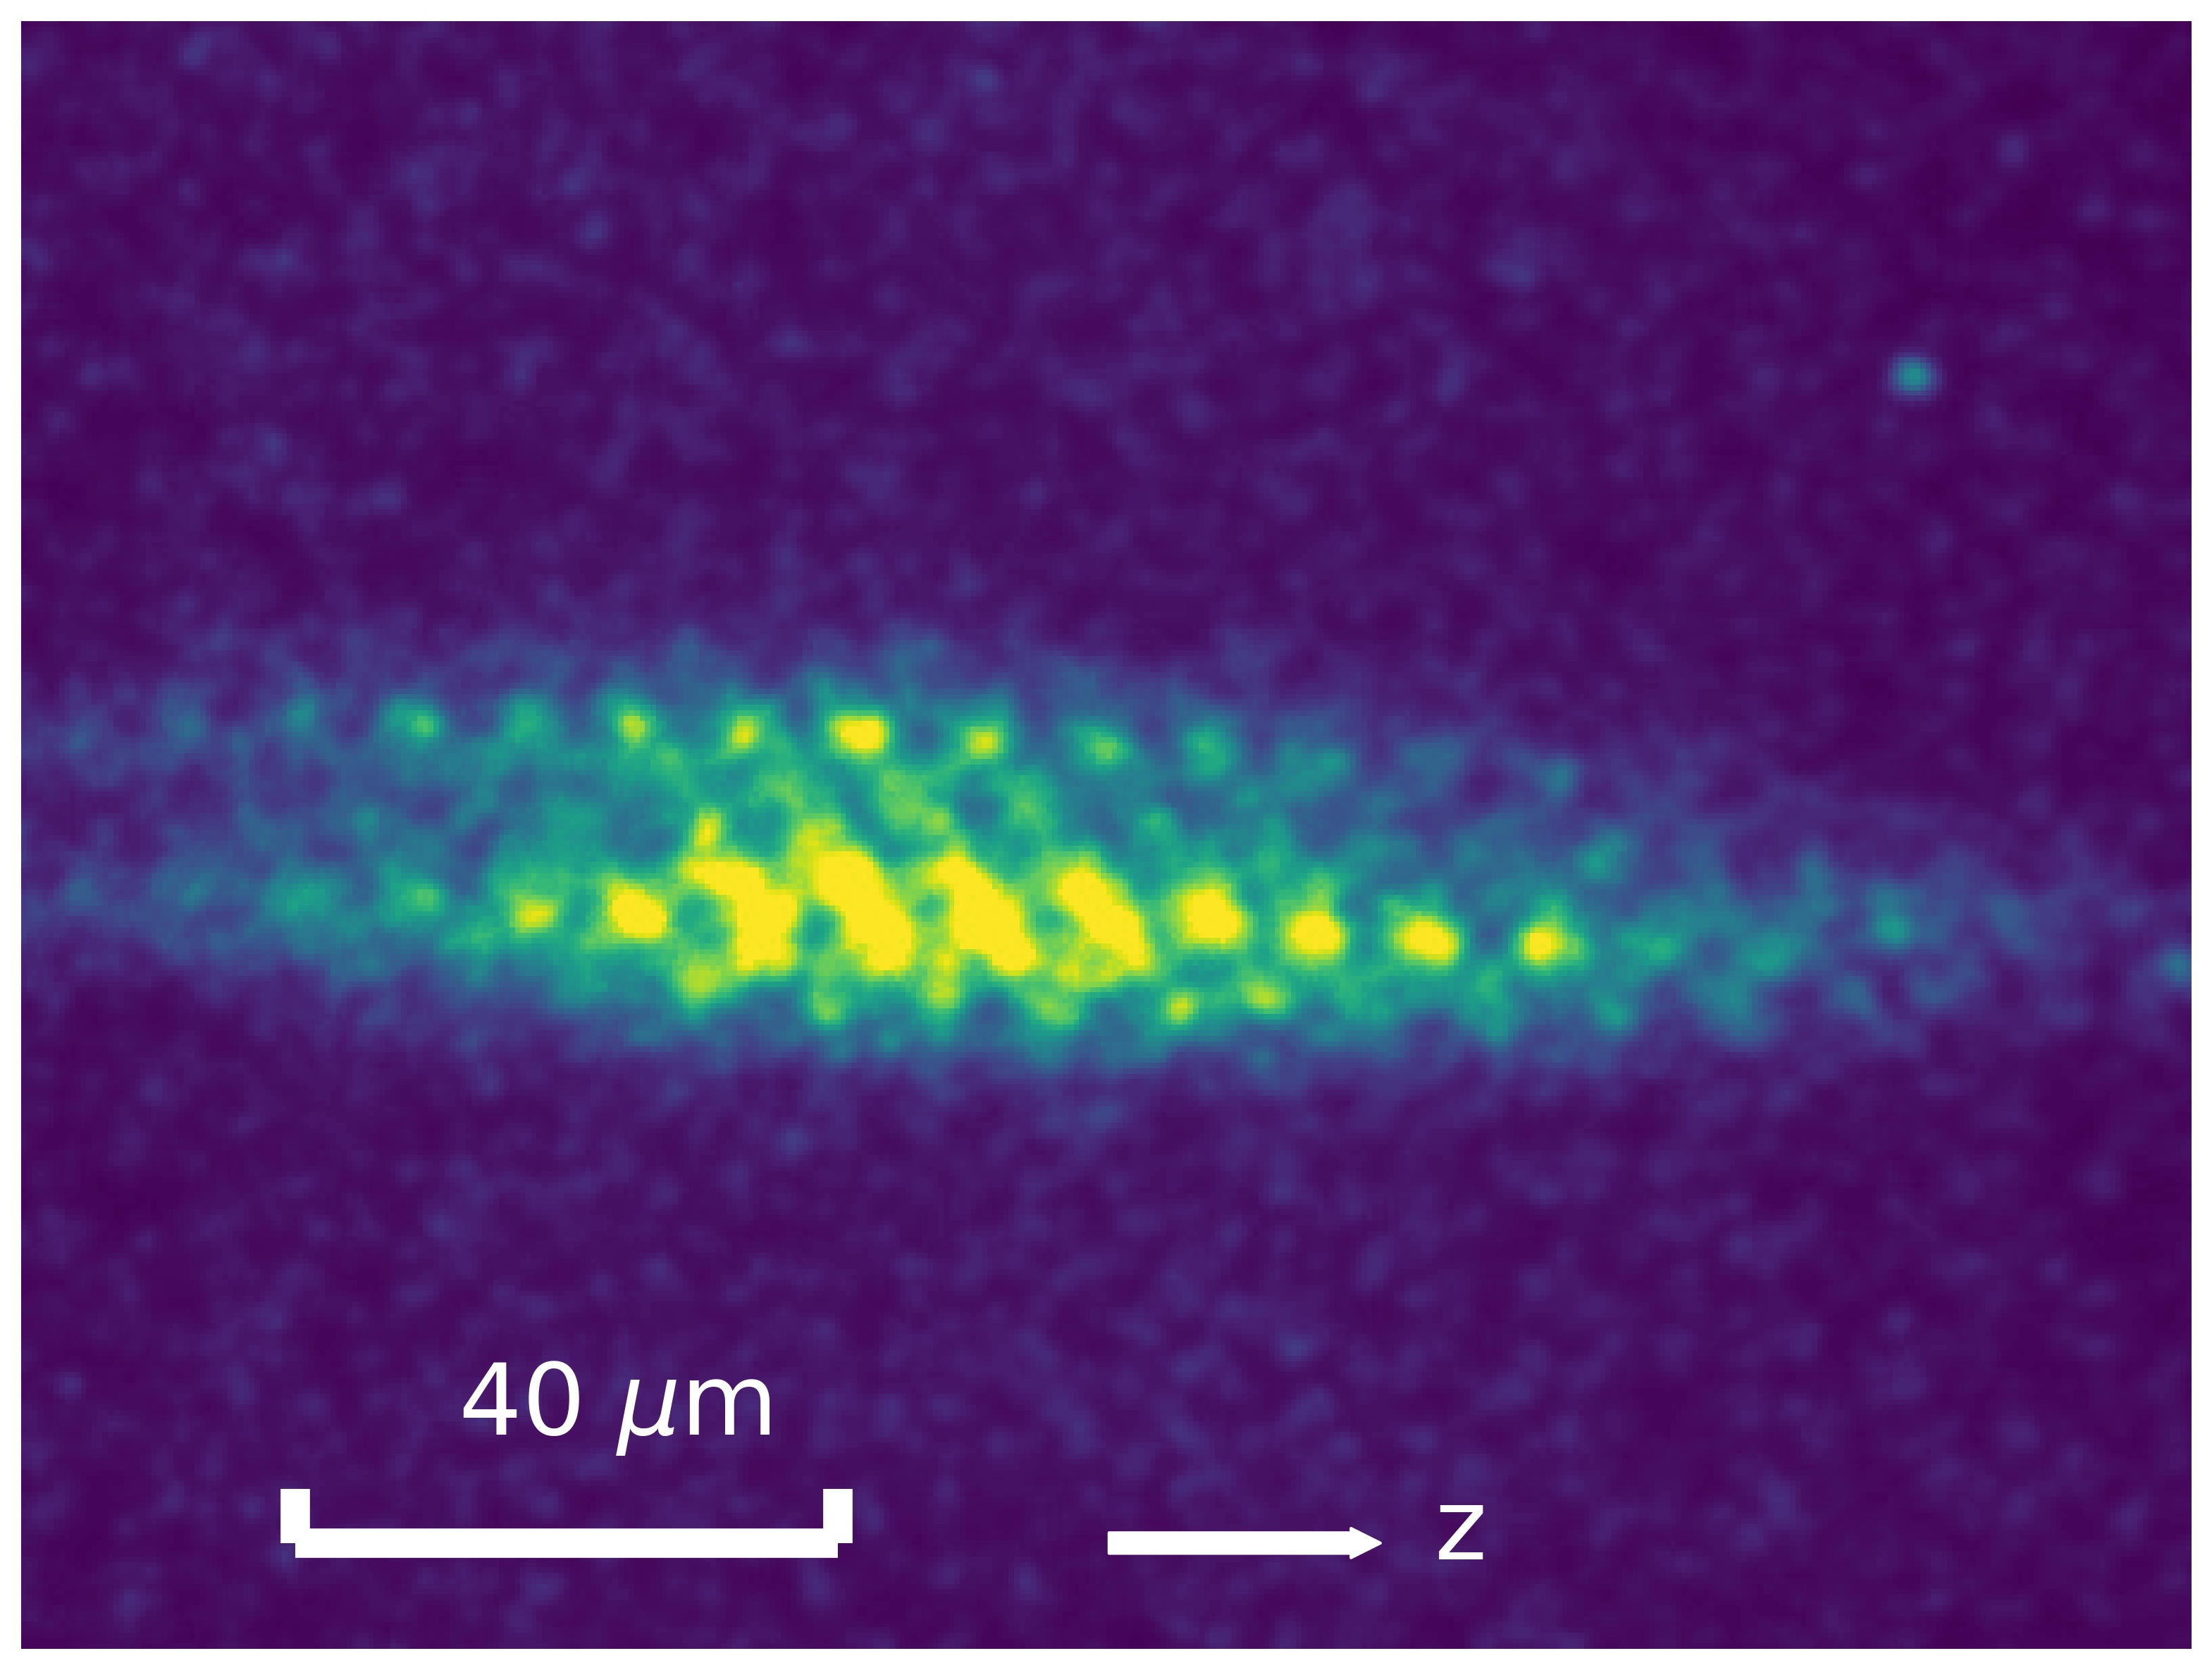
\includegraphics[width = 0.6\columnwidth]{./methods/figure/1_2D.jpg}
		\caption{手順1. でのイオン捕獲画像}
		\label{fig:1_2D}
	\end{center}
	\end{minipage}
	\begin{minipage}{0.48\linewidth}
		\begin{center}
			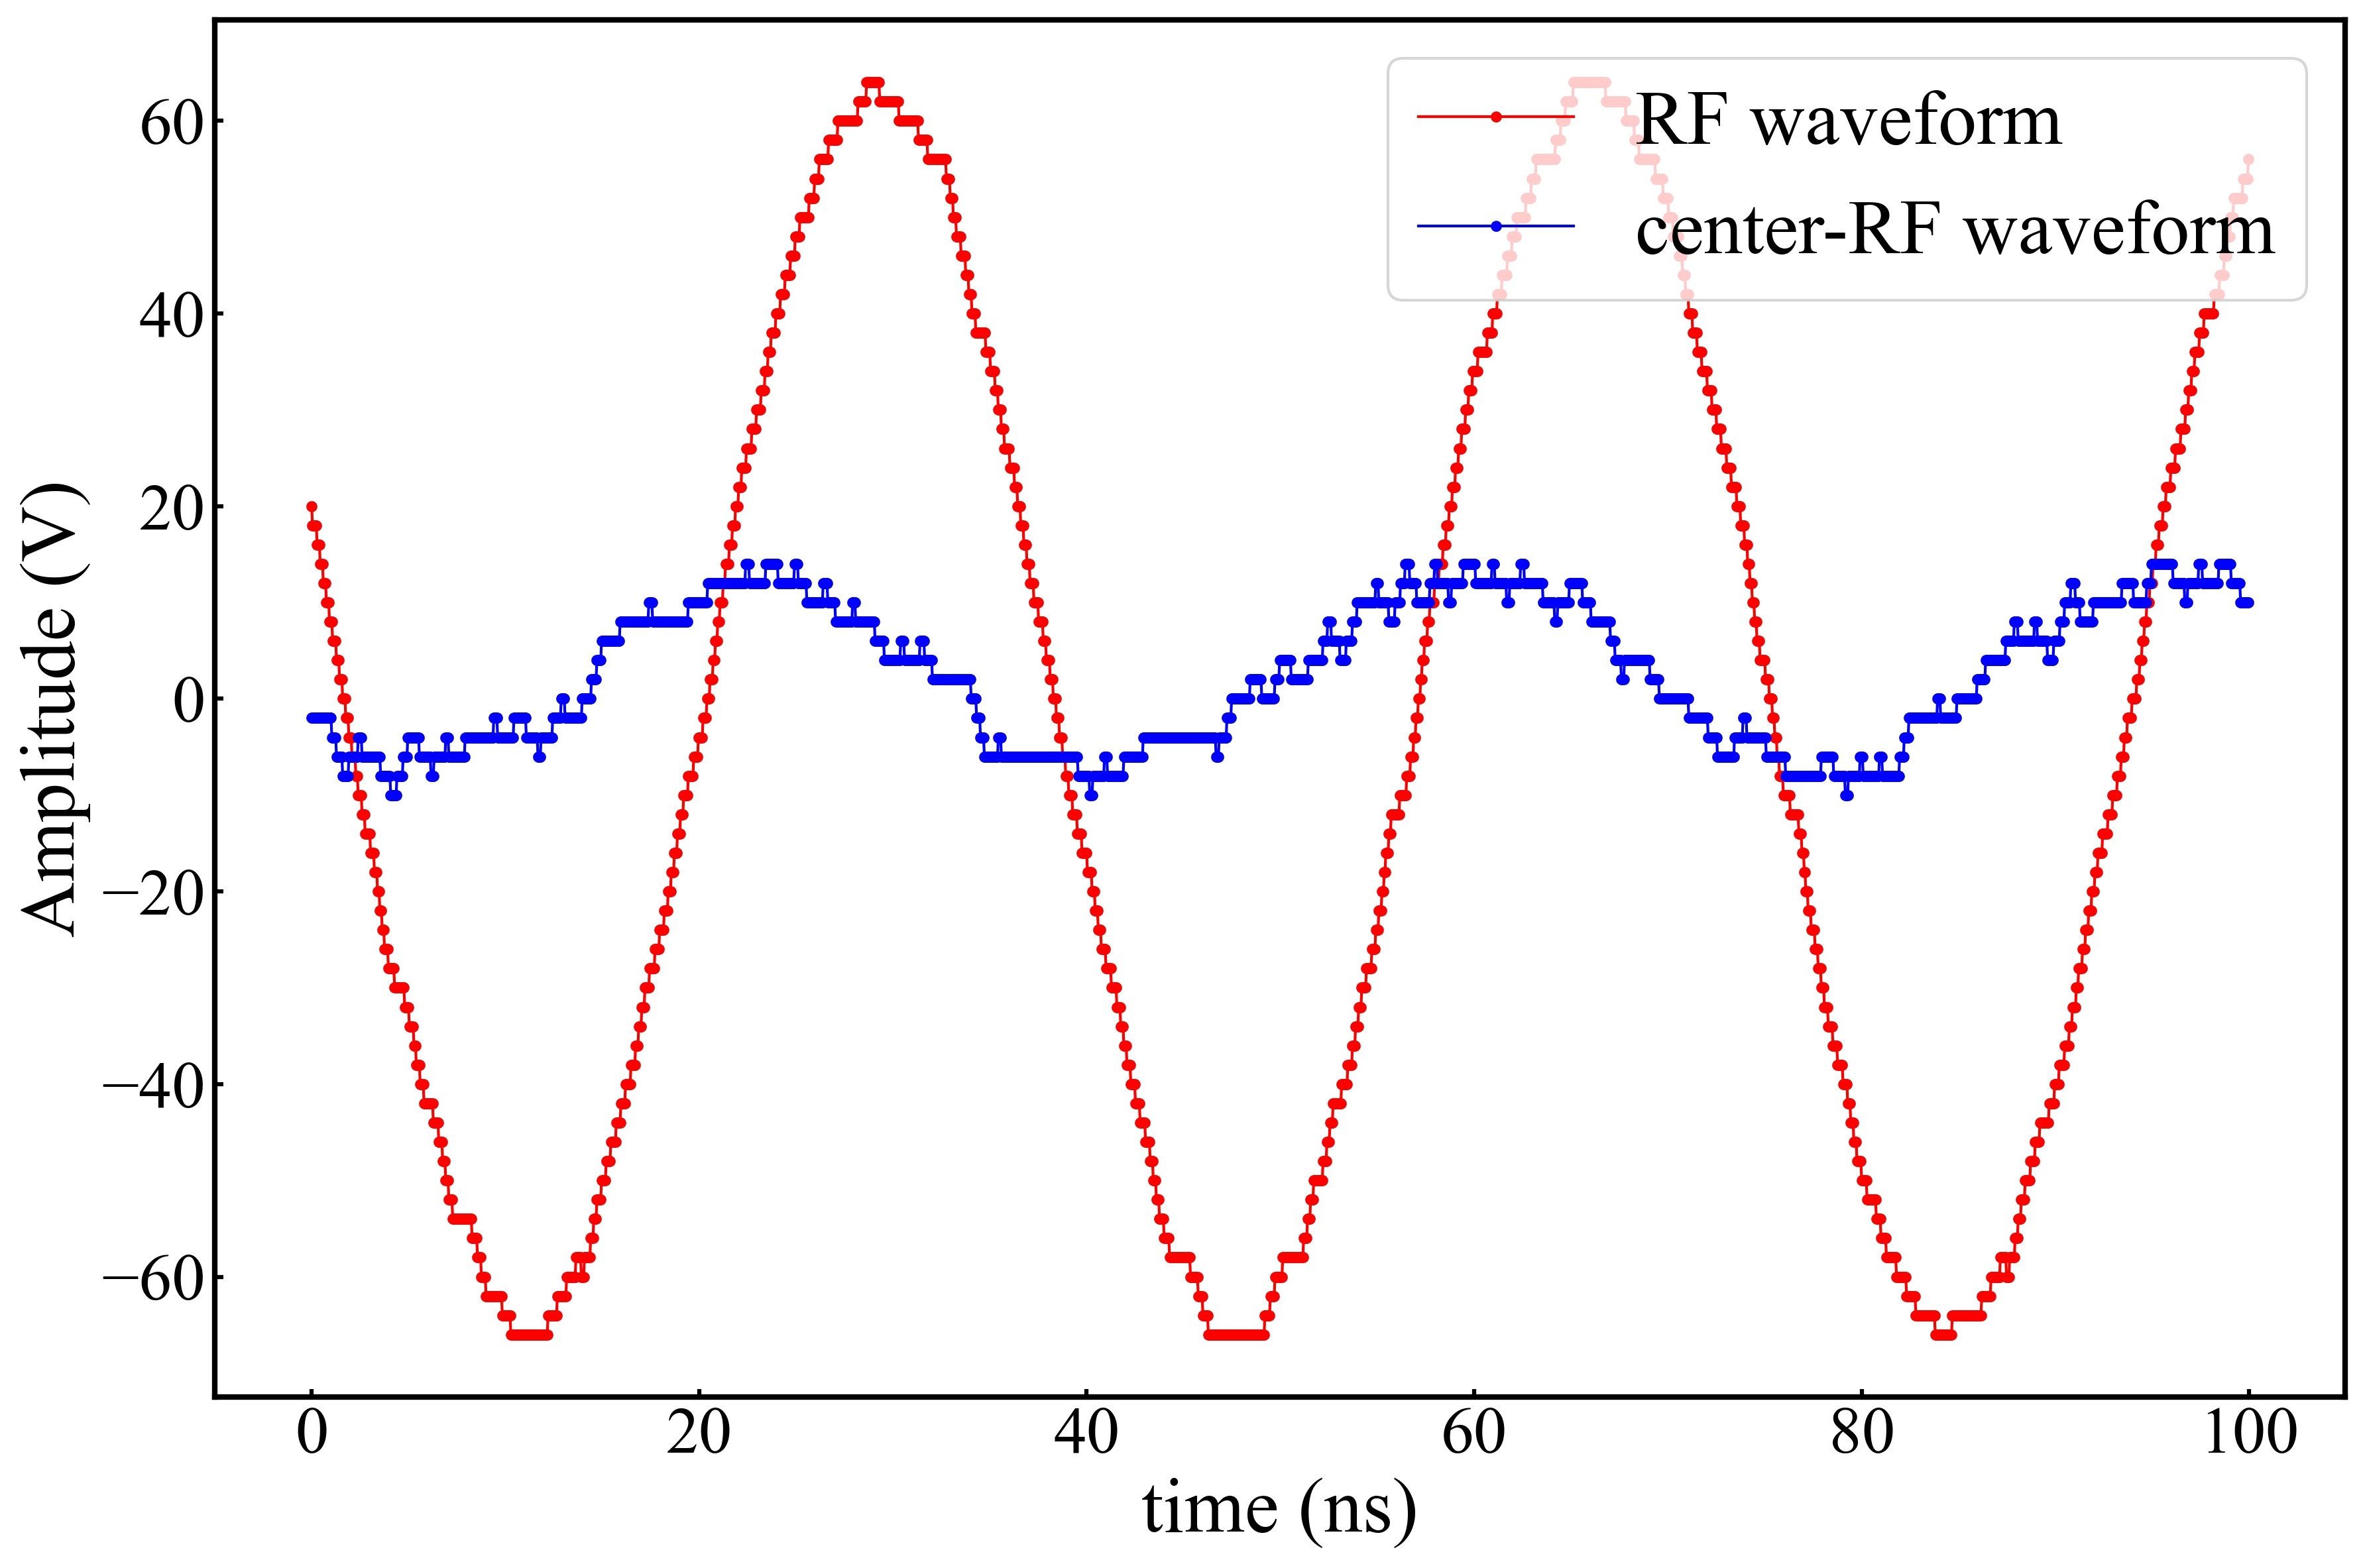
\includegraphics[width = 0.9\columnwidth]{./methods/figure/1_2D_wave.jpg}
			\caption{手順1. におけるrf電圧とcenter-rf電圧の関係}
			\label{fig:1_2D_wave}
		\end{center}
	\end{minipage}
\end{figure}

このとき,$R=0.21$となっている.また,マイクロメータの初期目盛を\Tb{1_2D}に示す.

\begin{table}[h]
	\begin{center}
	\caption{手順1. におけるマイクロメーターの初期目盛}
	\label{tab:1_2D}
	\begin{tabular}{c|cc} \hline \hline
		&鉛直方向&水平方向 \\ \hline
		垂直照射&39 &4 \\ 
		斜め照射&10&0 \\ \hline
	\end{tabular}
	\end{center}
\end{table}

\item 次に,center-rf電圧の振幅を発振器上で100 mVppに設定する.1. と同様に\Fig{2_2D}にイオン捕獲画像,\Fig{2_2D_wave}にrf電圧とcenter-rf電圧の関係を示す.\\
%
\clearpage
%
\begin{figure}[h]
	\begin{minipage}{0.48\linewidth}
	\begin{center}
		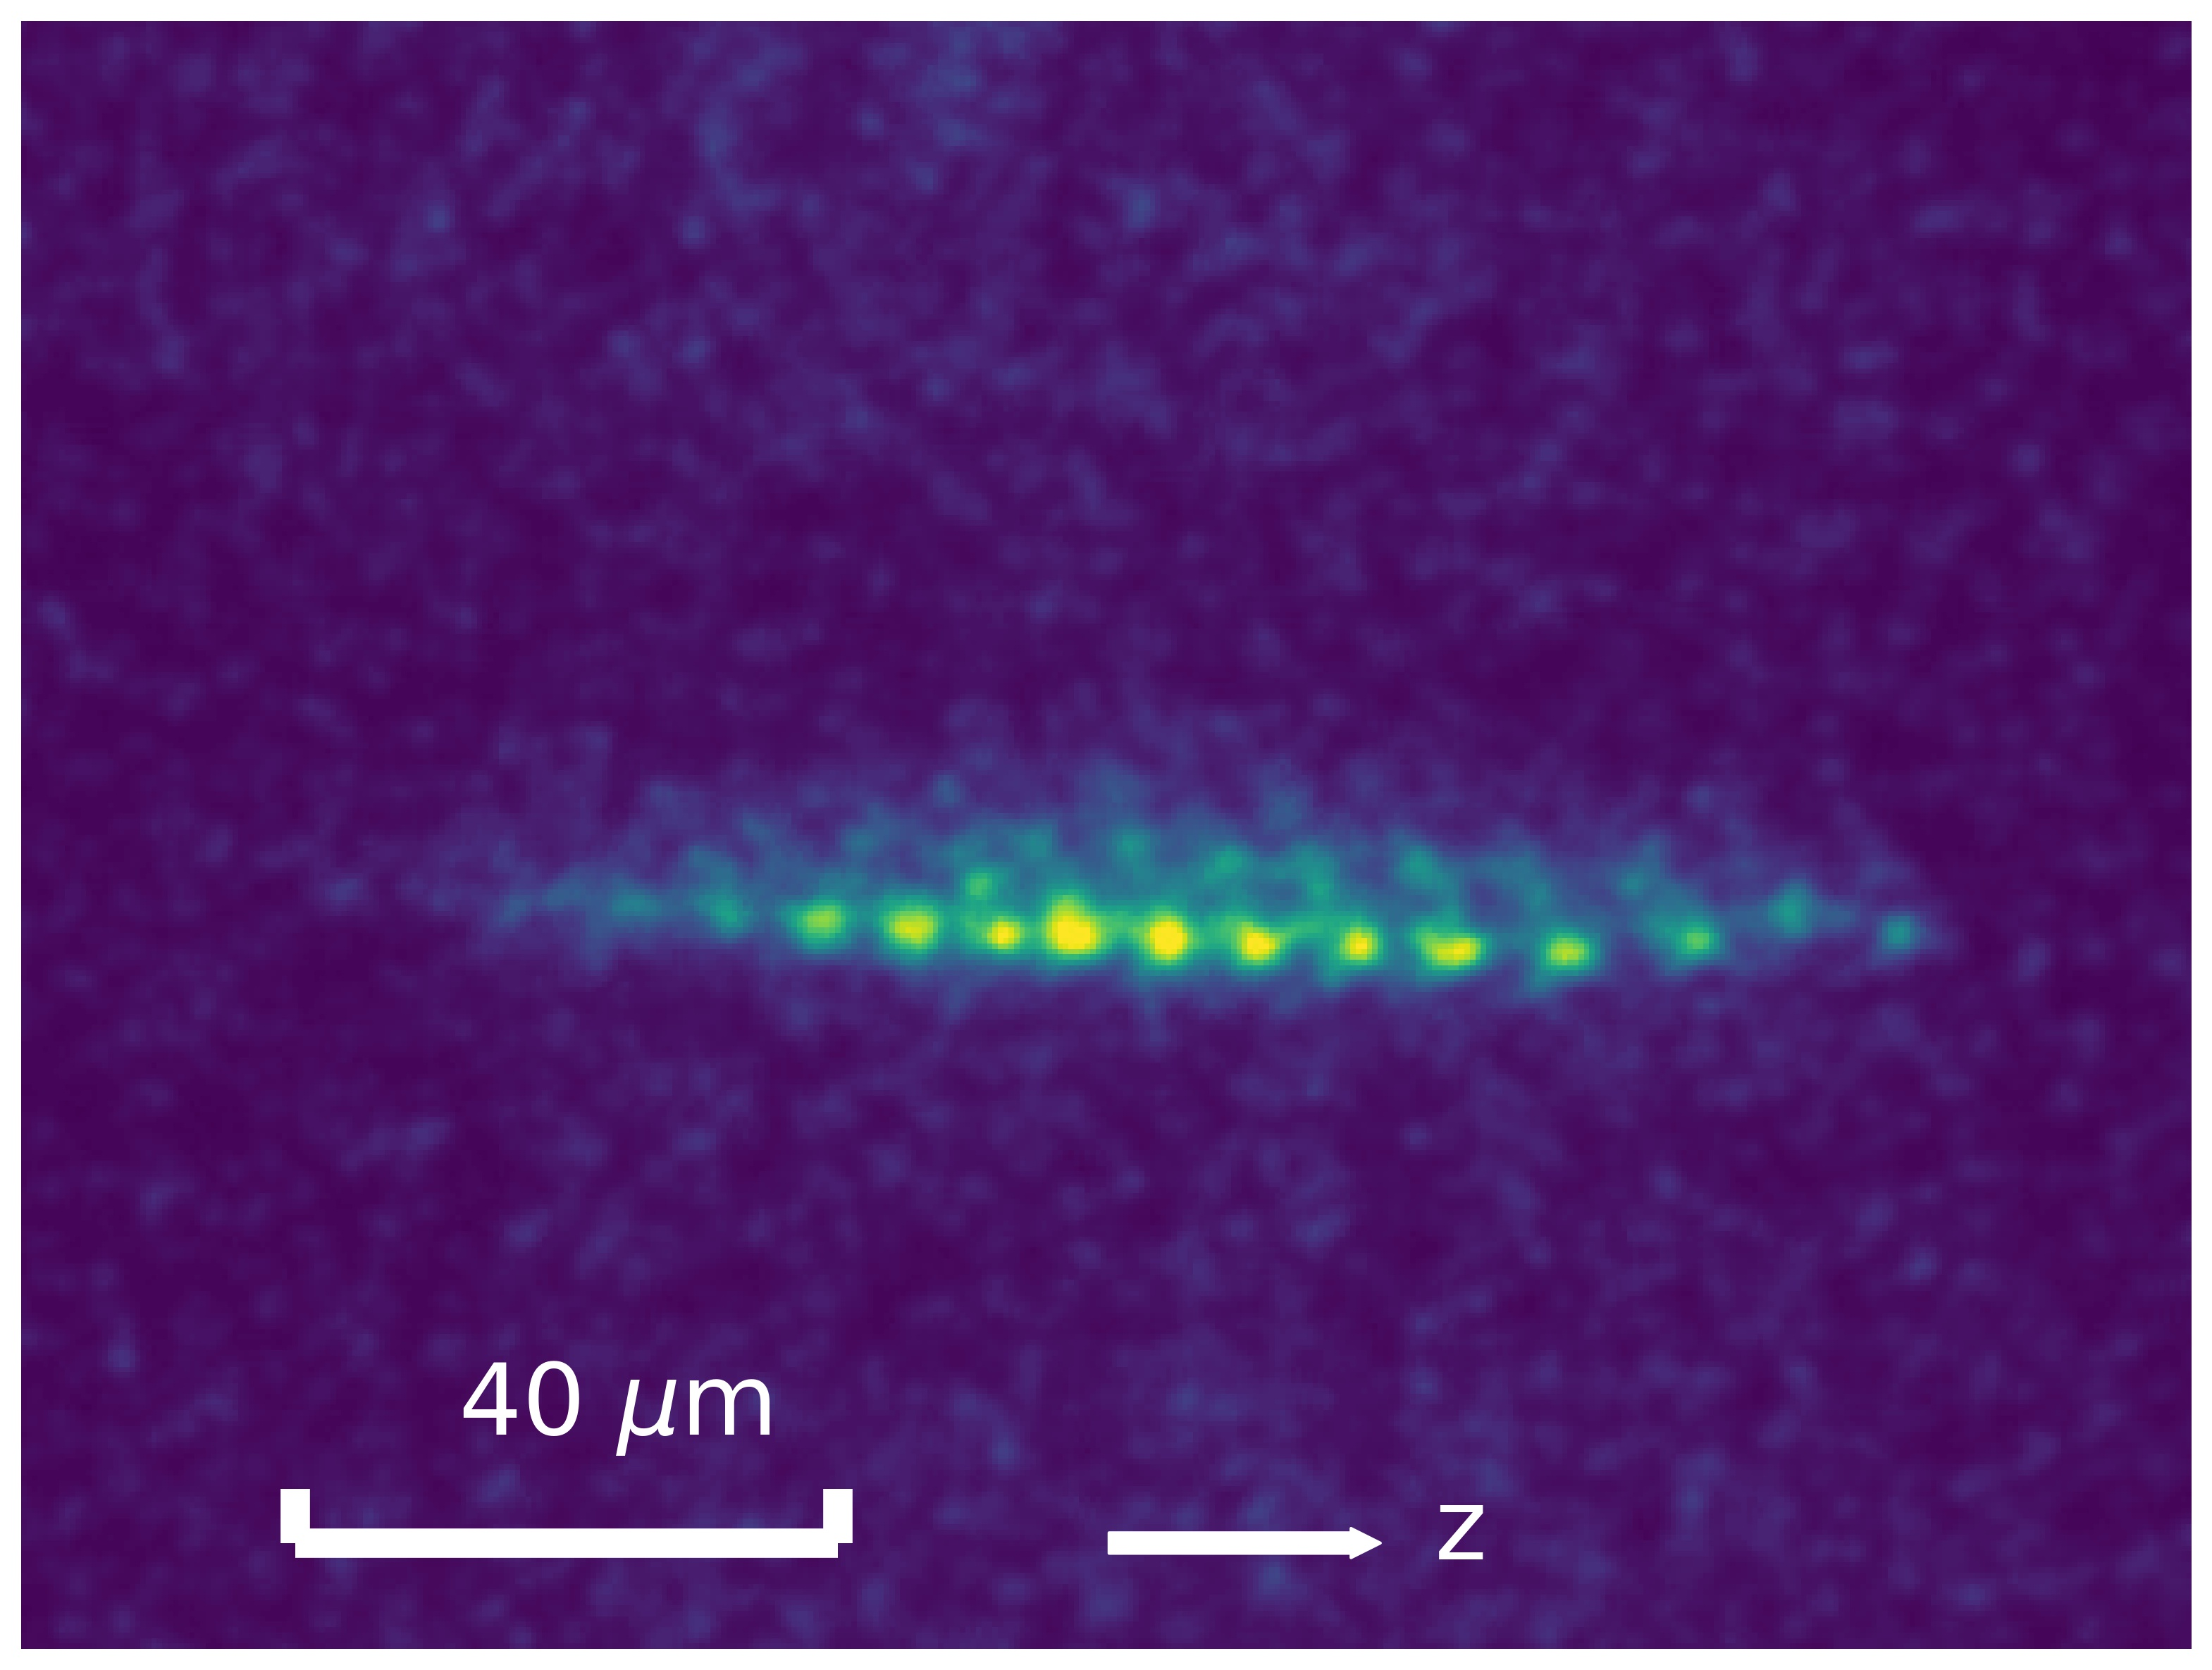
\includegraphics[width = 0.6\columnwidth]{./methods/figure/2_2D.jpg}
		\caption{手順2. でのイオン捕獲画像}
		\label{fig:2_2D}
	\end{center}
	\end{minipage}
	\begin{minipage}{0.48\linewidth}
		\begin{center}
			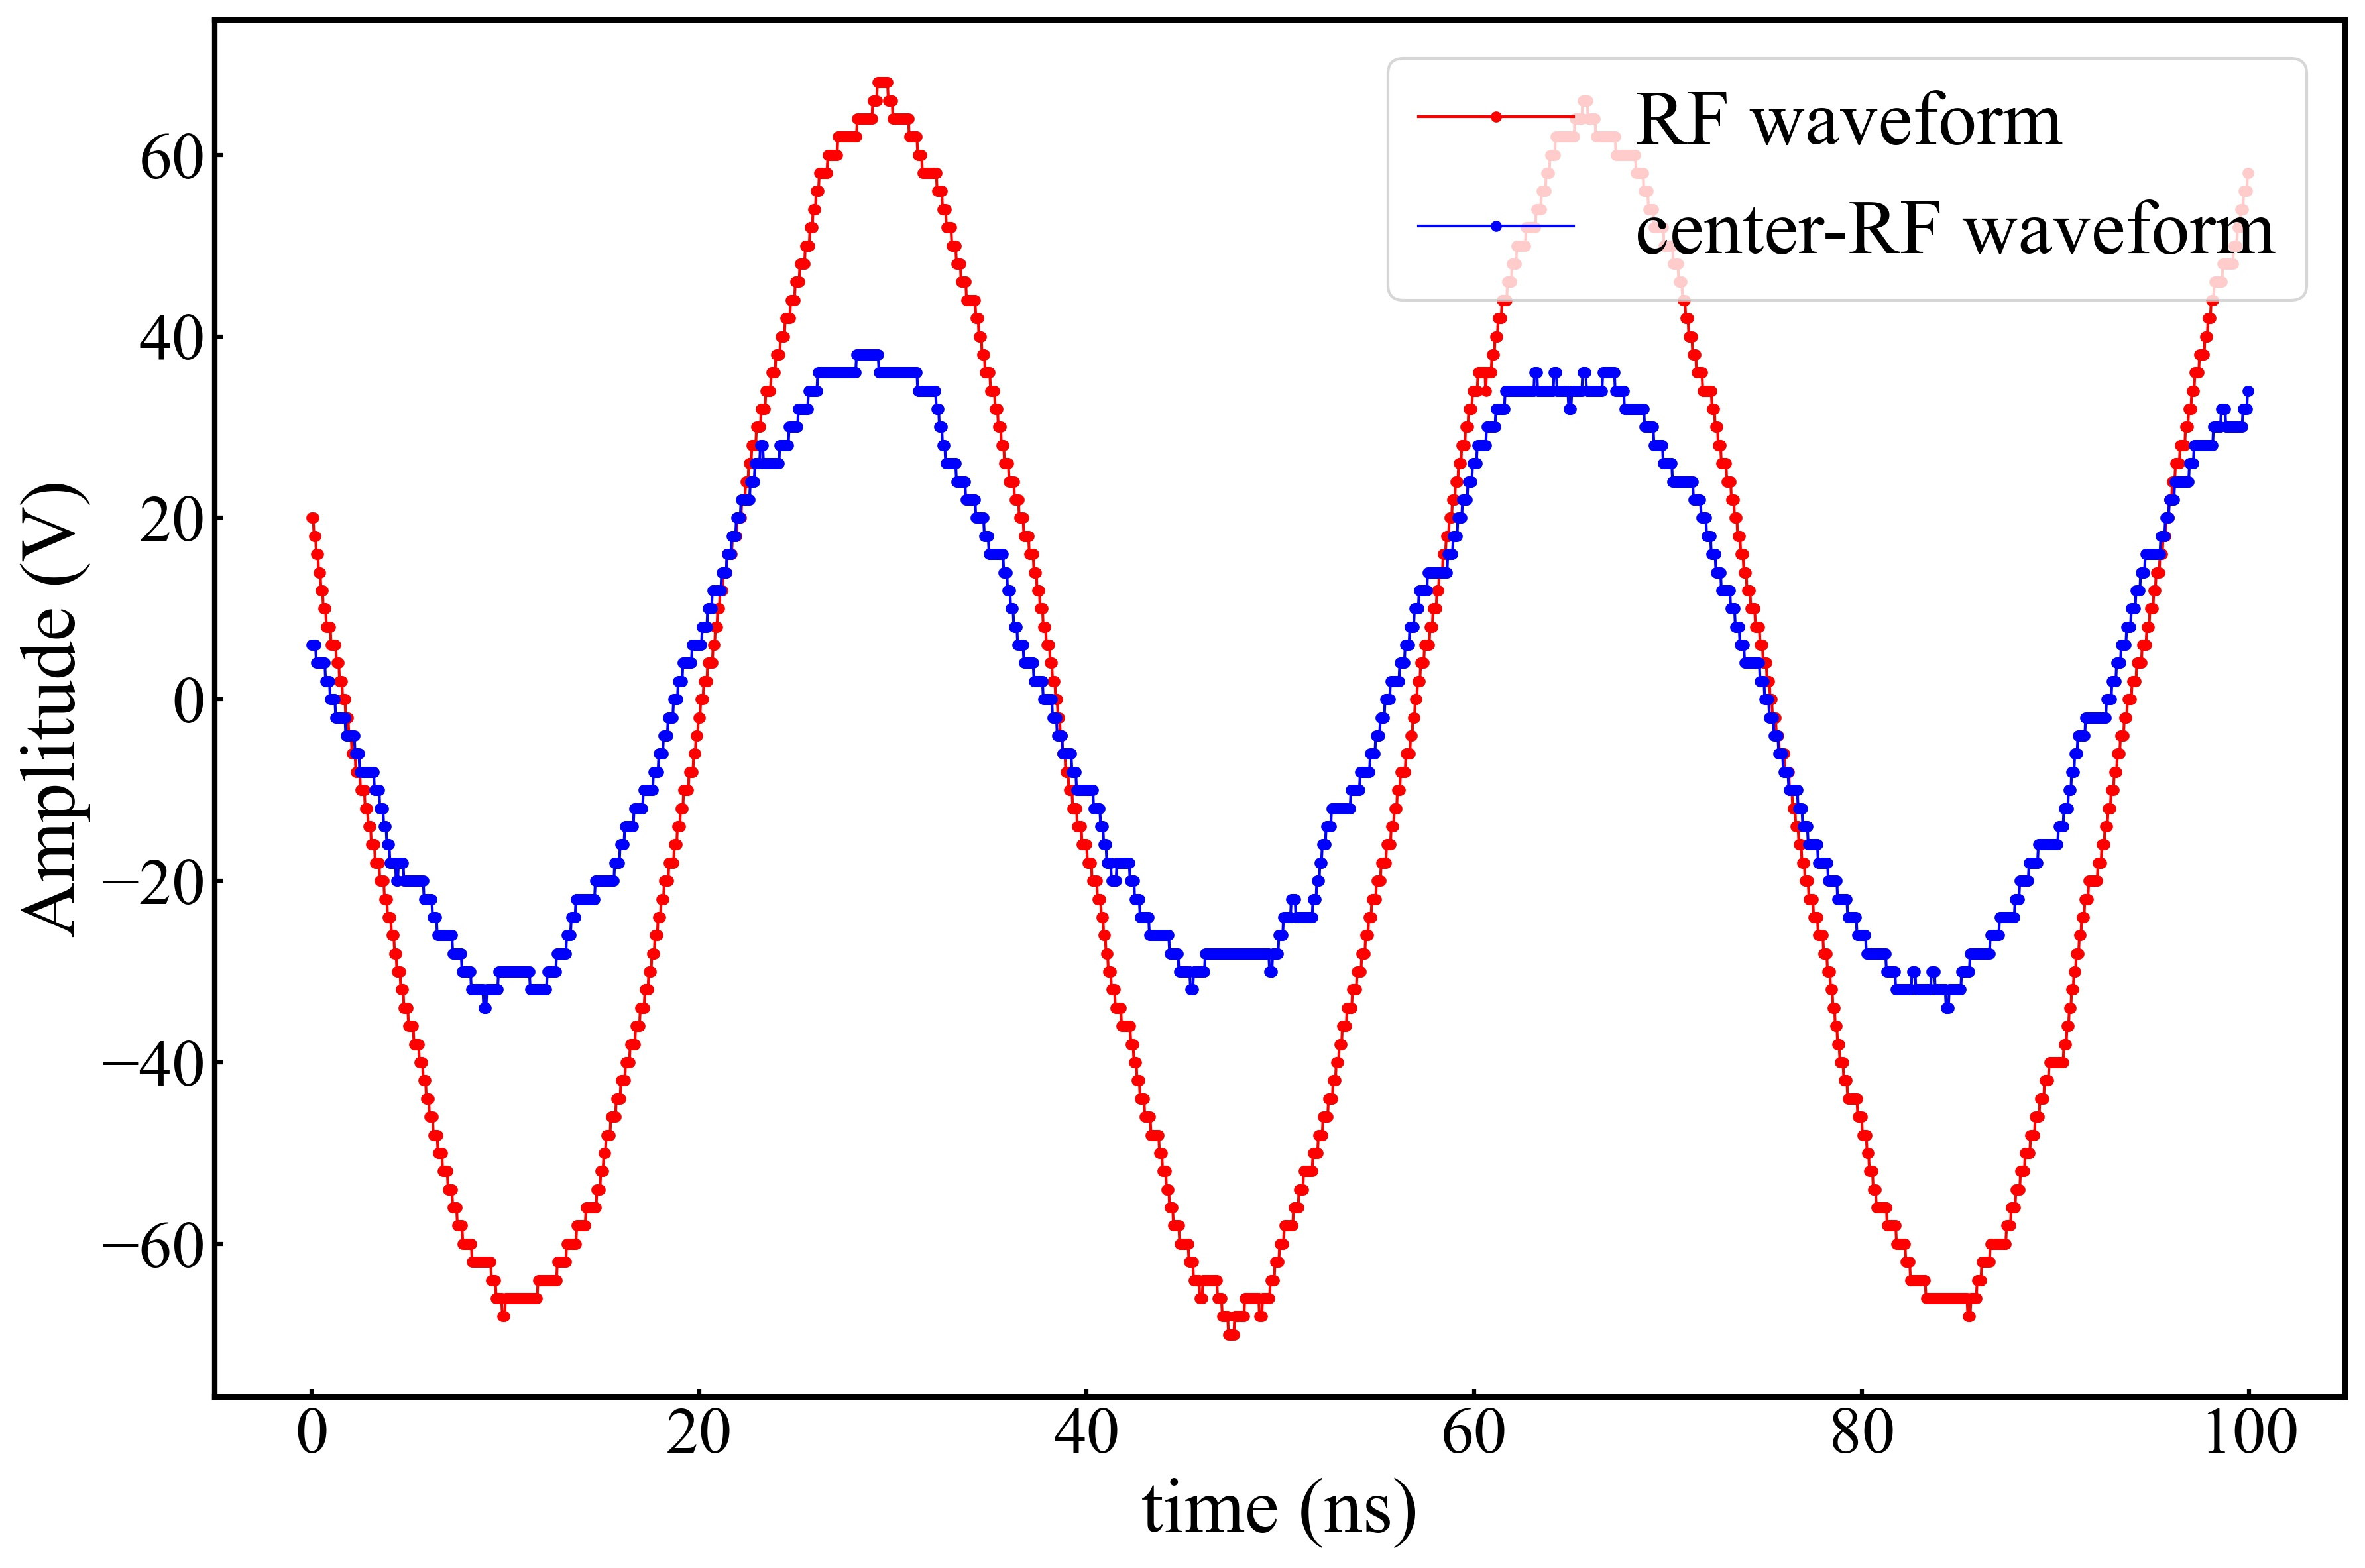
\includegraphics[width = 0.9\columnwidth]{./methods/figure/2_2D_wave.jpg}
			\caption{手順2. におけるrf電圧とcenter-rf電圧の関係}
			\label{fig:2_2D_wave}
		\end{center}
	\end{minipage}
\end{figure}

このとき,$R=0.56$である.手順1. $\rightarrow$ 手順2. で変化させたマイクロメータの変位を\Tb{2_2D}に示す.

\begin{table}[h]
\begin{center}
	\caption{手順1. $\rightarrow$ 手順1. で変化させたマイクロメータの変位}
	\label{tab:2_2D}
	\begin{tabular}{c|cc} \hline \hline
		&鉛直方向への変位&水平方向の変位 \\ \hline
		垂直照射&-4 $\mu$m & +3 $\mu$m \\ 
		斜め照射&-5 $\mu$m & +3 $\mu$m \\ \hline
	\end{tabular}
\end{center}
\end{table}

イオン捕獲位置がプレーナートラップ表面に近づき,レンズの位置がそれぞれ鉛直方向について下がることから,イオンの蛍光がはっきりと観測されるようにピントの調節を行っている.
\item 発振器上でcenter-rf電圧を135 mVppに設定する.\Fig{3_2D}にイオン捕獲画像,\Fig{3_2D_wave}にrf電圧とcenter-rf電圧の関係を示す.

\begin{figure}[h]
	\begin{minipage}{0.48\linewidth}
	\begin{center}
		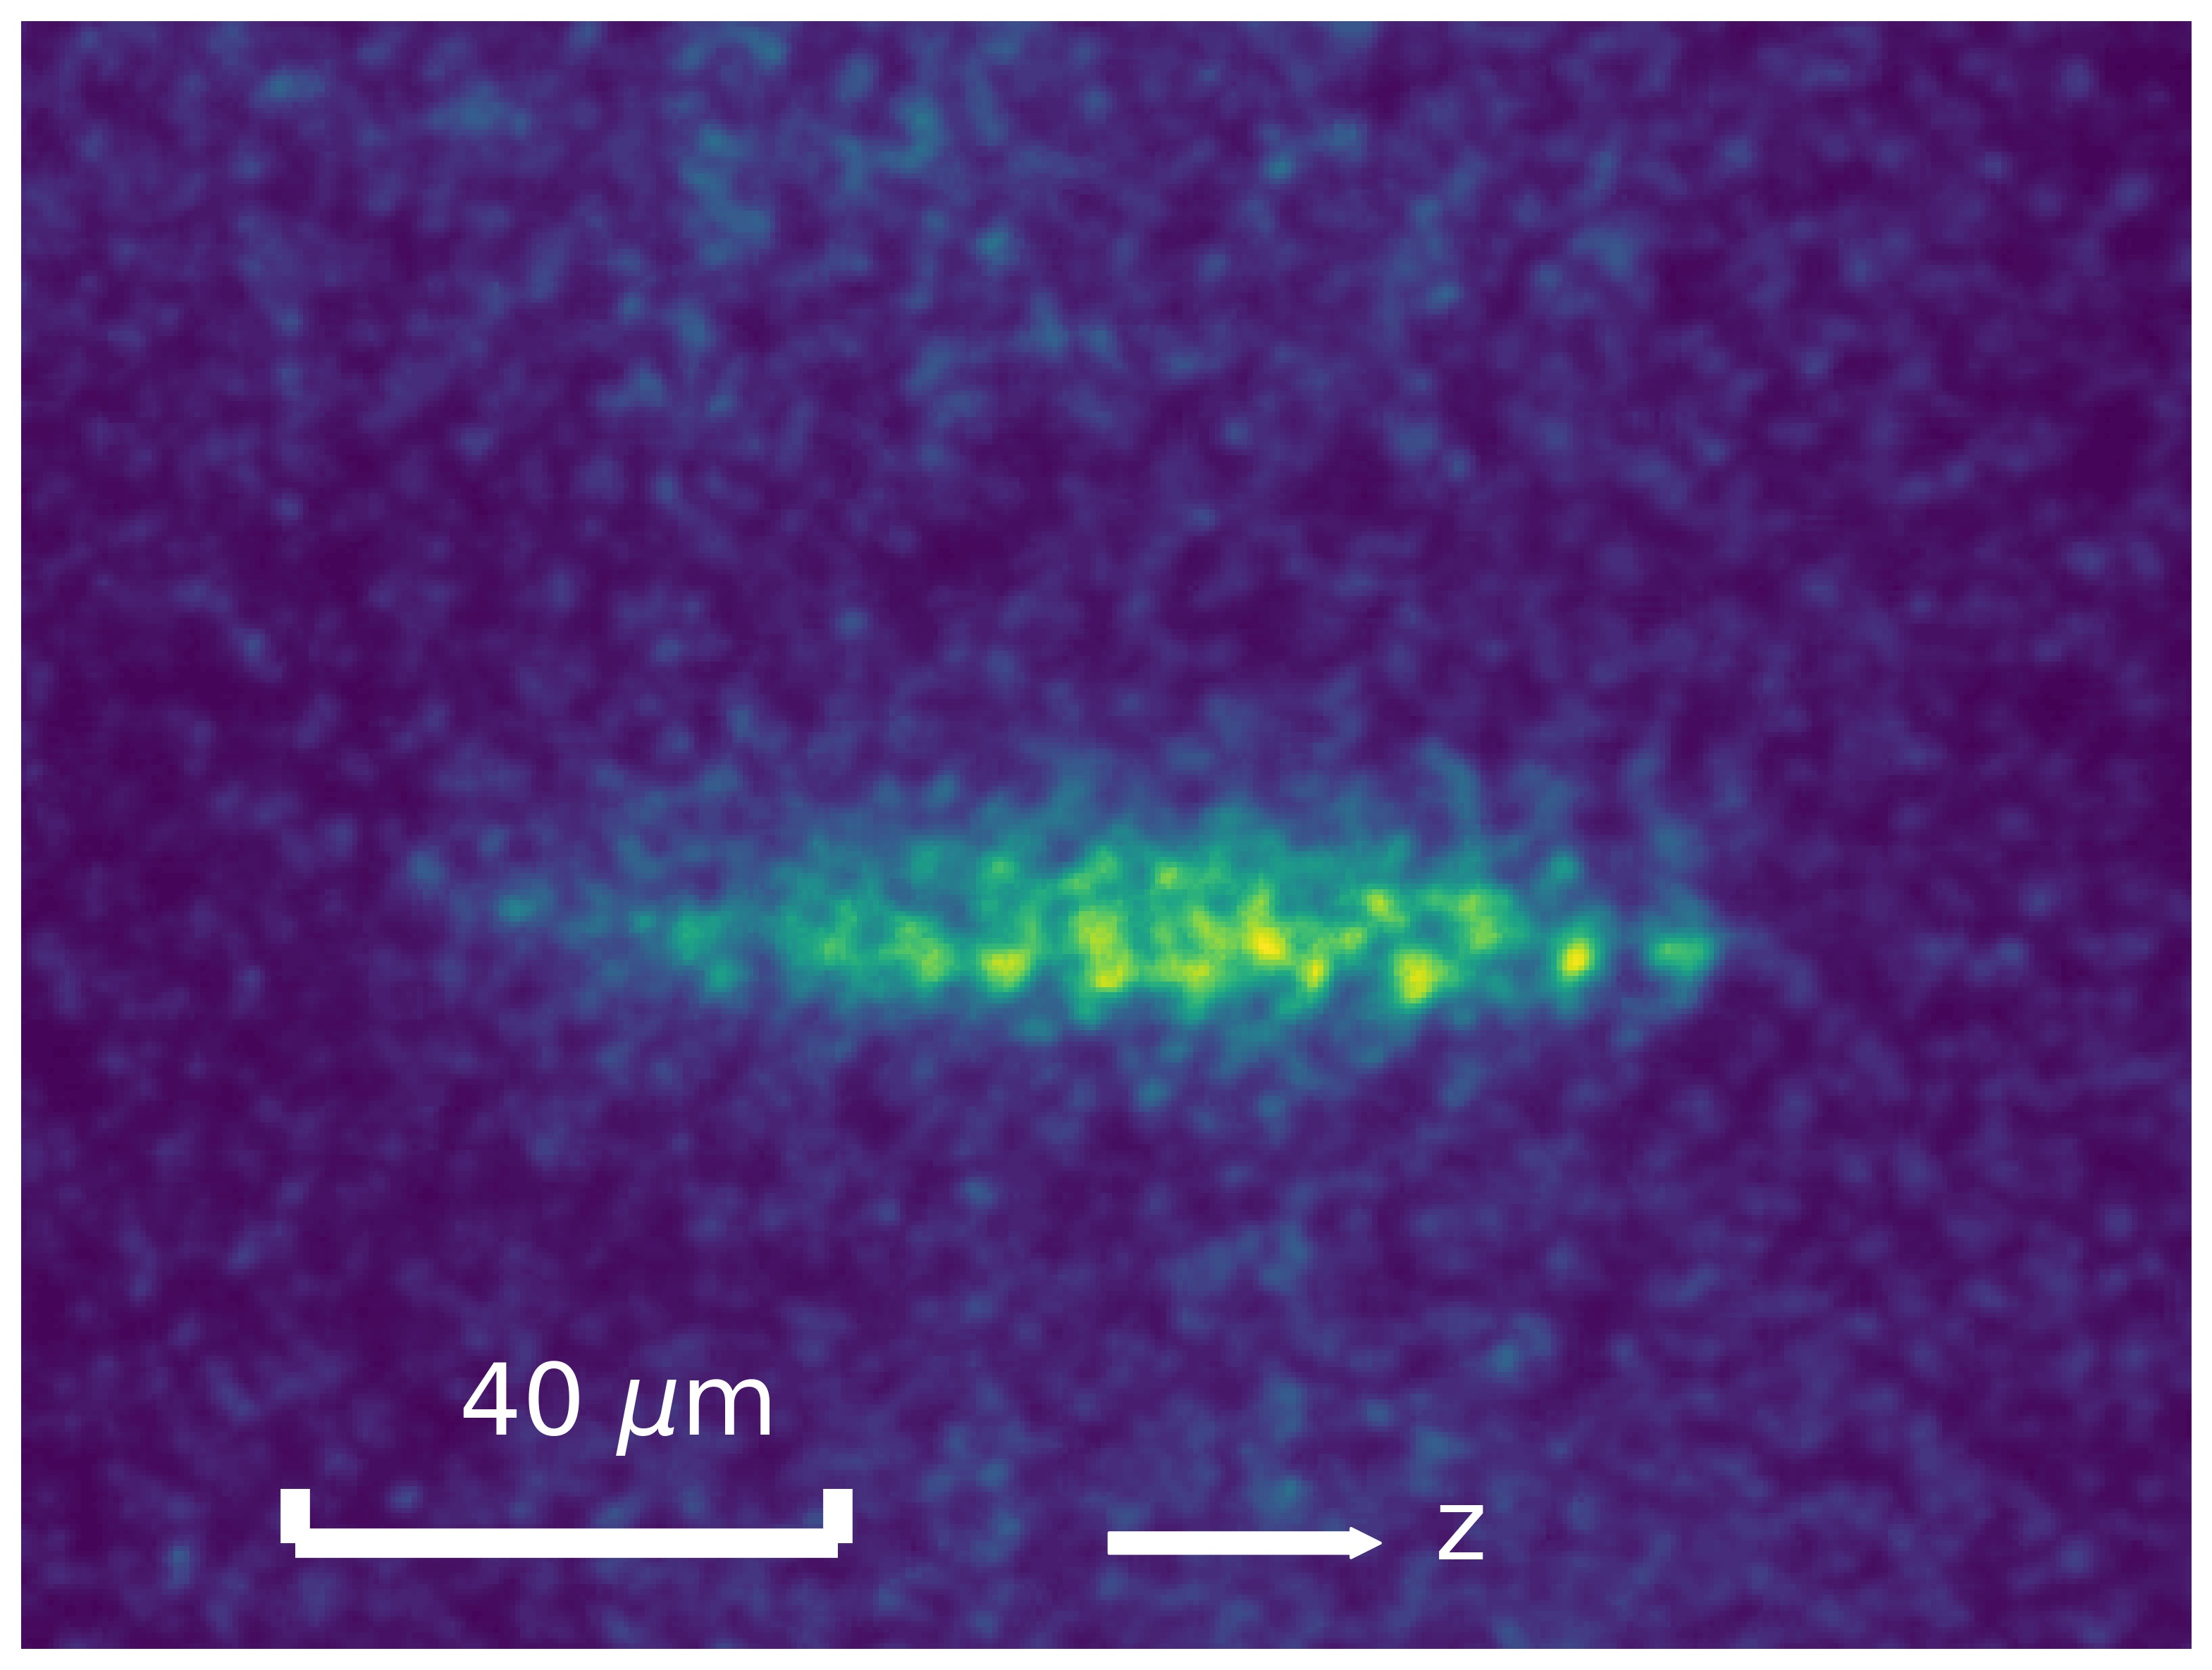
\includegraphics[width = 0.6\columnwidth]{./methods/figure/3_2D.jpg}
		\caption{手順3. でのイオン捕獲画像}
		\label{fig:3_2D}
	\end{center}
	\end{minipage}
	\begin{minipage}{0.48\linewidth}
		\begin{center}
			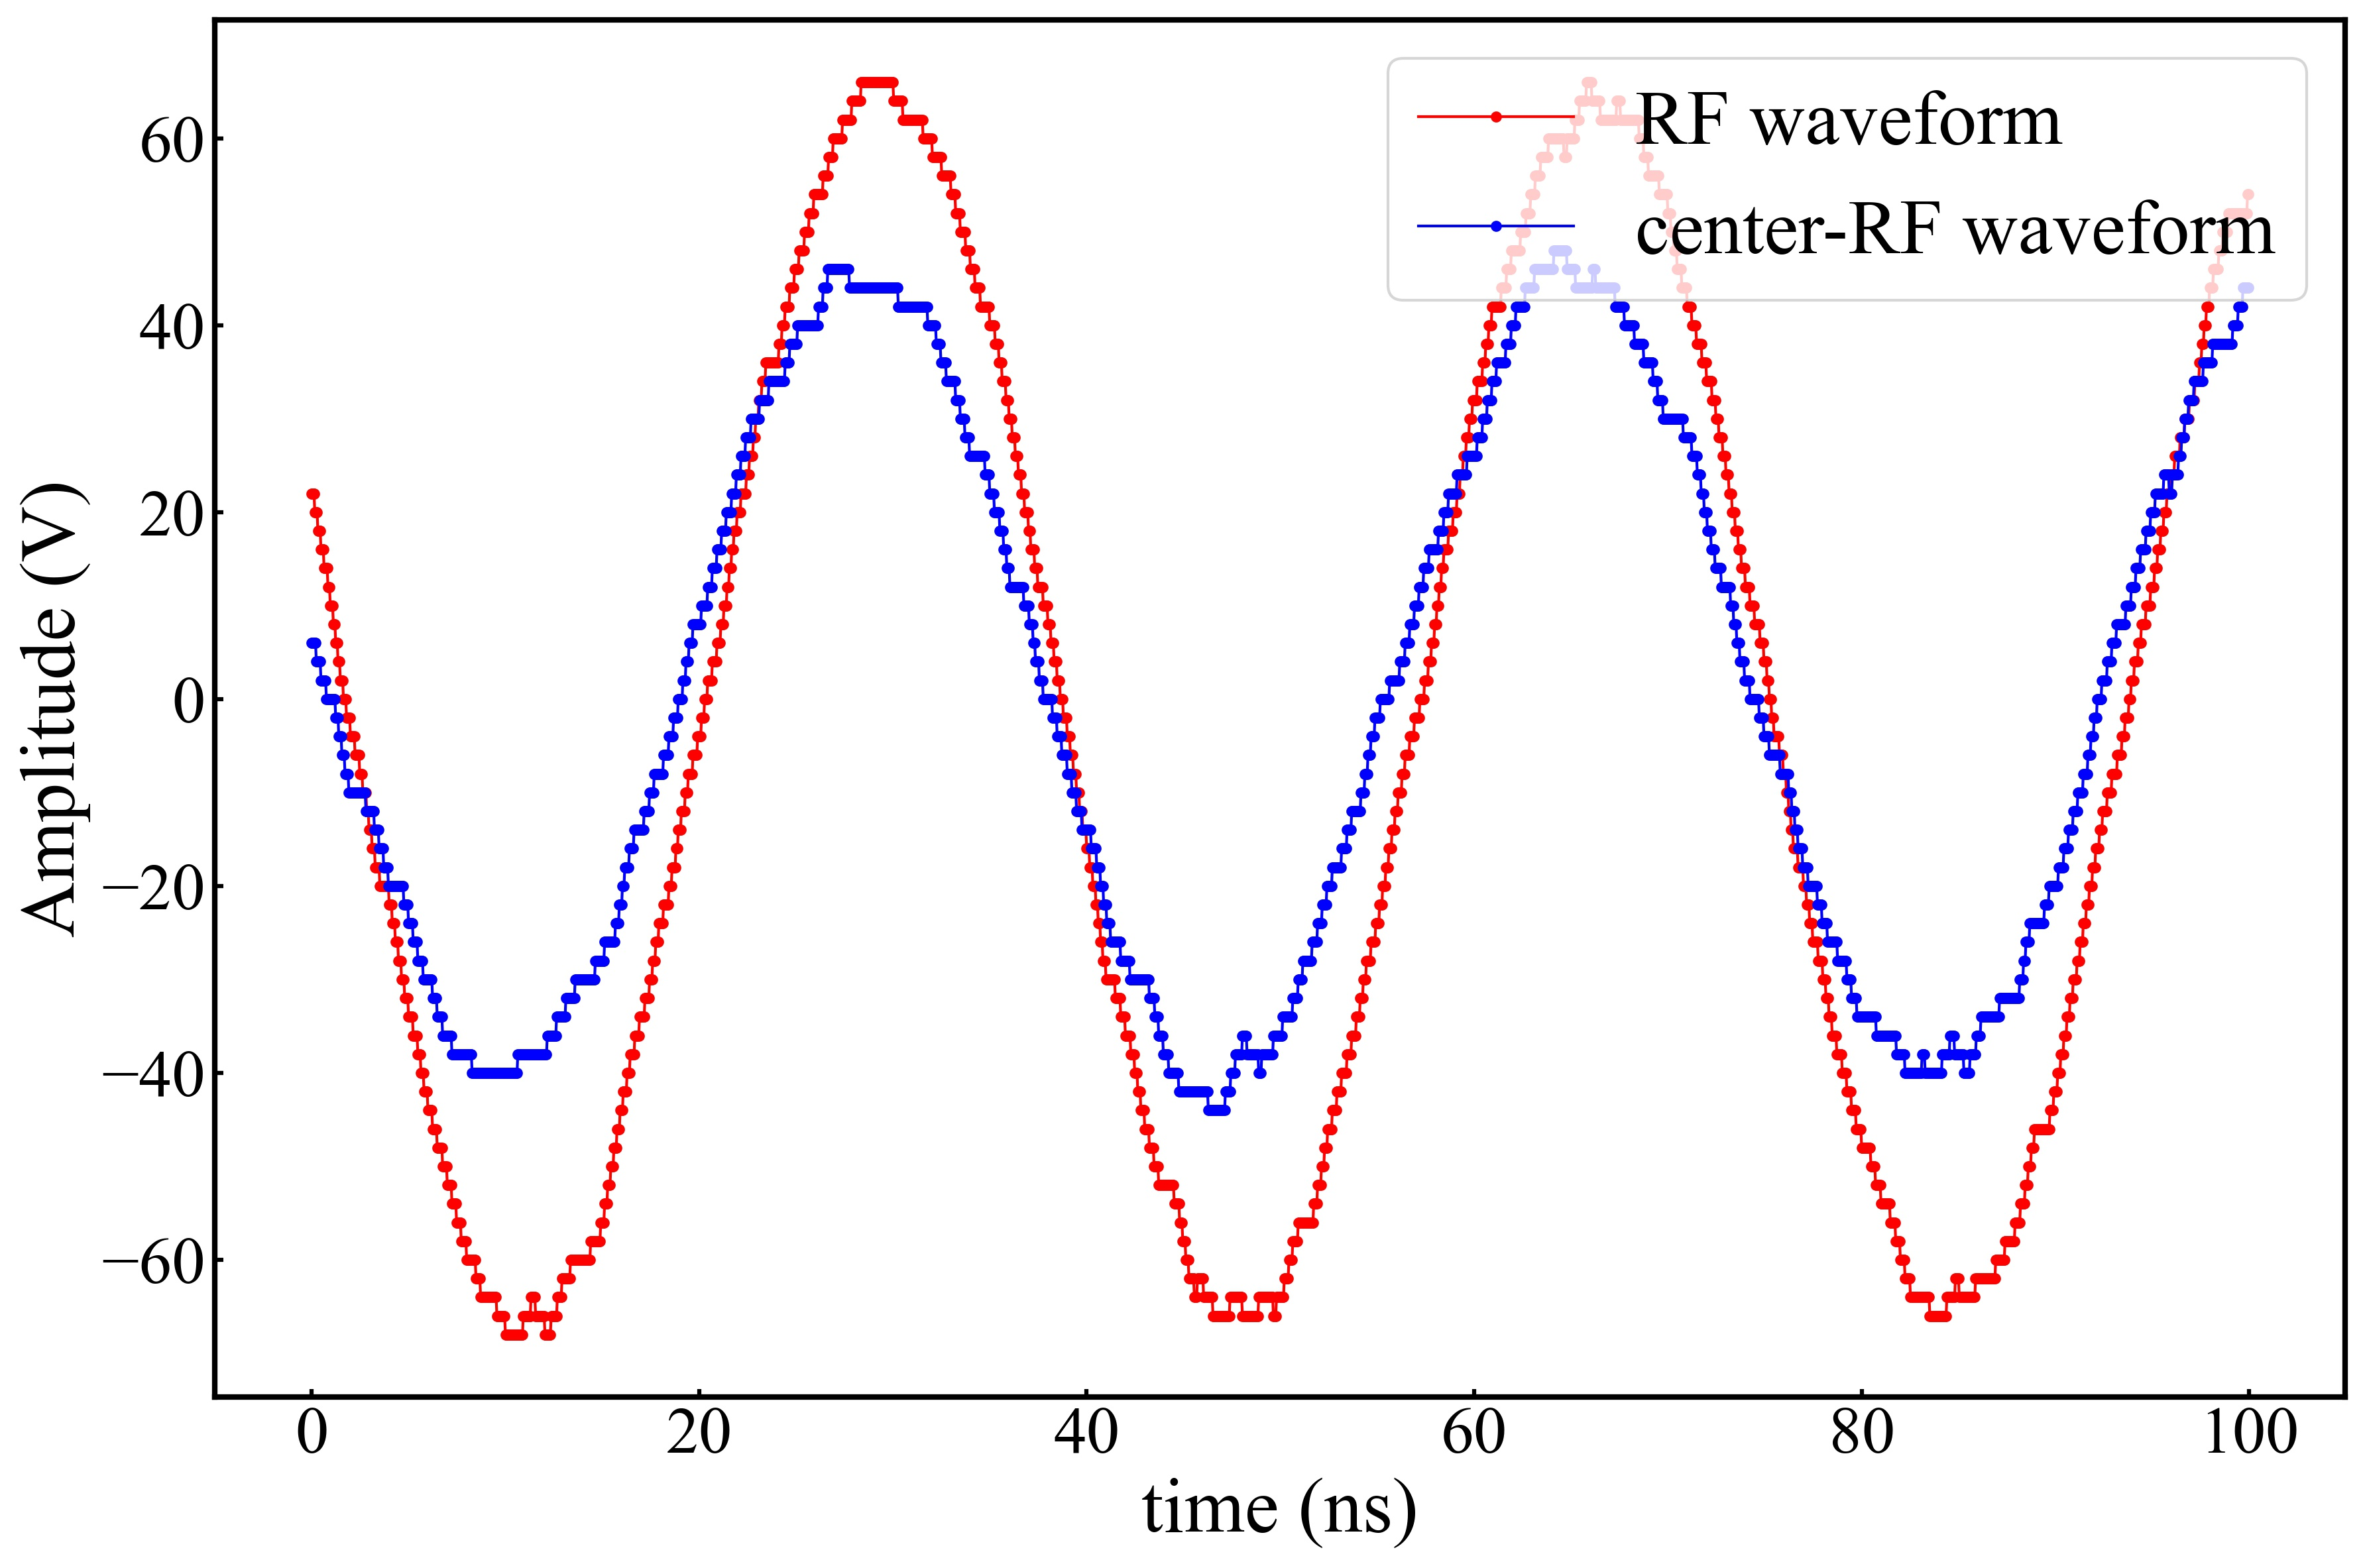
\includegraphics[width = 0.9\columnwidth]{./methods/figure/3_2D_wave.jpg}
			\caption{手順3. におけるrf電圧とcenter-rf電圧の関係}
			\label{fig:3_2D_wave}
		\end{center}
	\end{minipage}
\end{figure}

このとき,$R=0.72$となっている.手順2. $\rightarrow$ 手順3. で変化させたマイクロメータの変位を\Tb{2_2D}に示す..

\begin{table}[h]
\begin{center}
	\caption{手順3. におけるレンズの位置を調節するマイクロメータの目盛}
	\label{tab:3_2D}
	\begin{tabular}{c|cc} \hline \hline
		&鉛直方向の変位&水平方向の変位 \\ \hline
		垂直照射&0 $\mu$m & 0 $\mu$m \\ 
		斜め照射&-3 $\mu$m & -2 $\mu$m \\ \hline
	\end{tabular}
\end{center}
\end{table}

この時点では,Double-wellポテンシャルの形成はまだ行われていない.

\item さらにcenter-rf電圧の振幅を175 mVppに上げる.\Fig{4_2D}にイオン捕獲画像を示し,\Fig{4_2D_wave}にrf電圧とcenter-rf電圧の関係を示す.

\begin{figure}[h]
	\begin{minipage}{0.48\linewidth}
	\begin{center}
		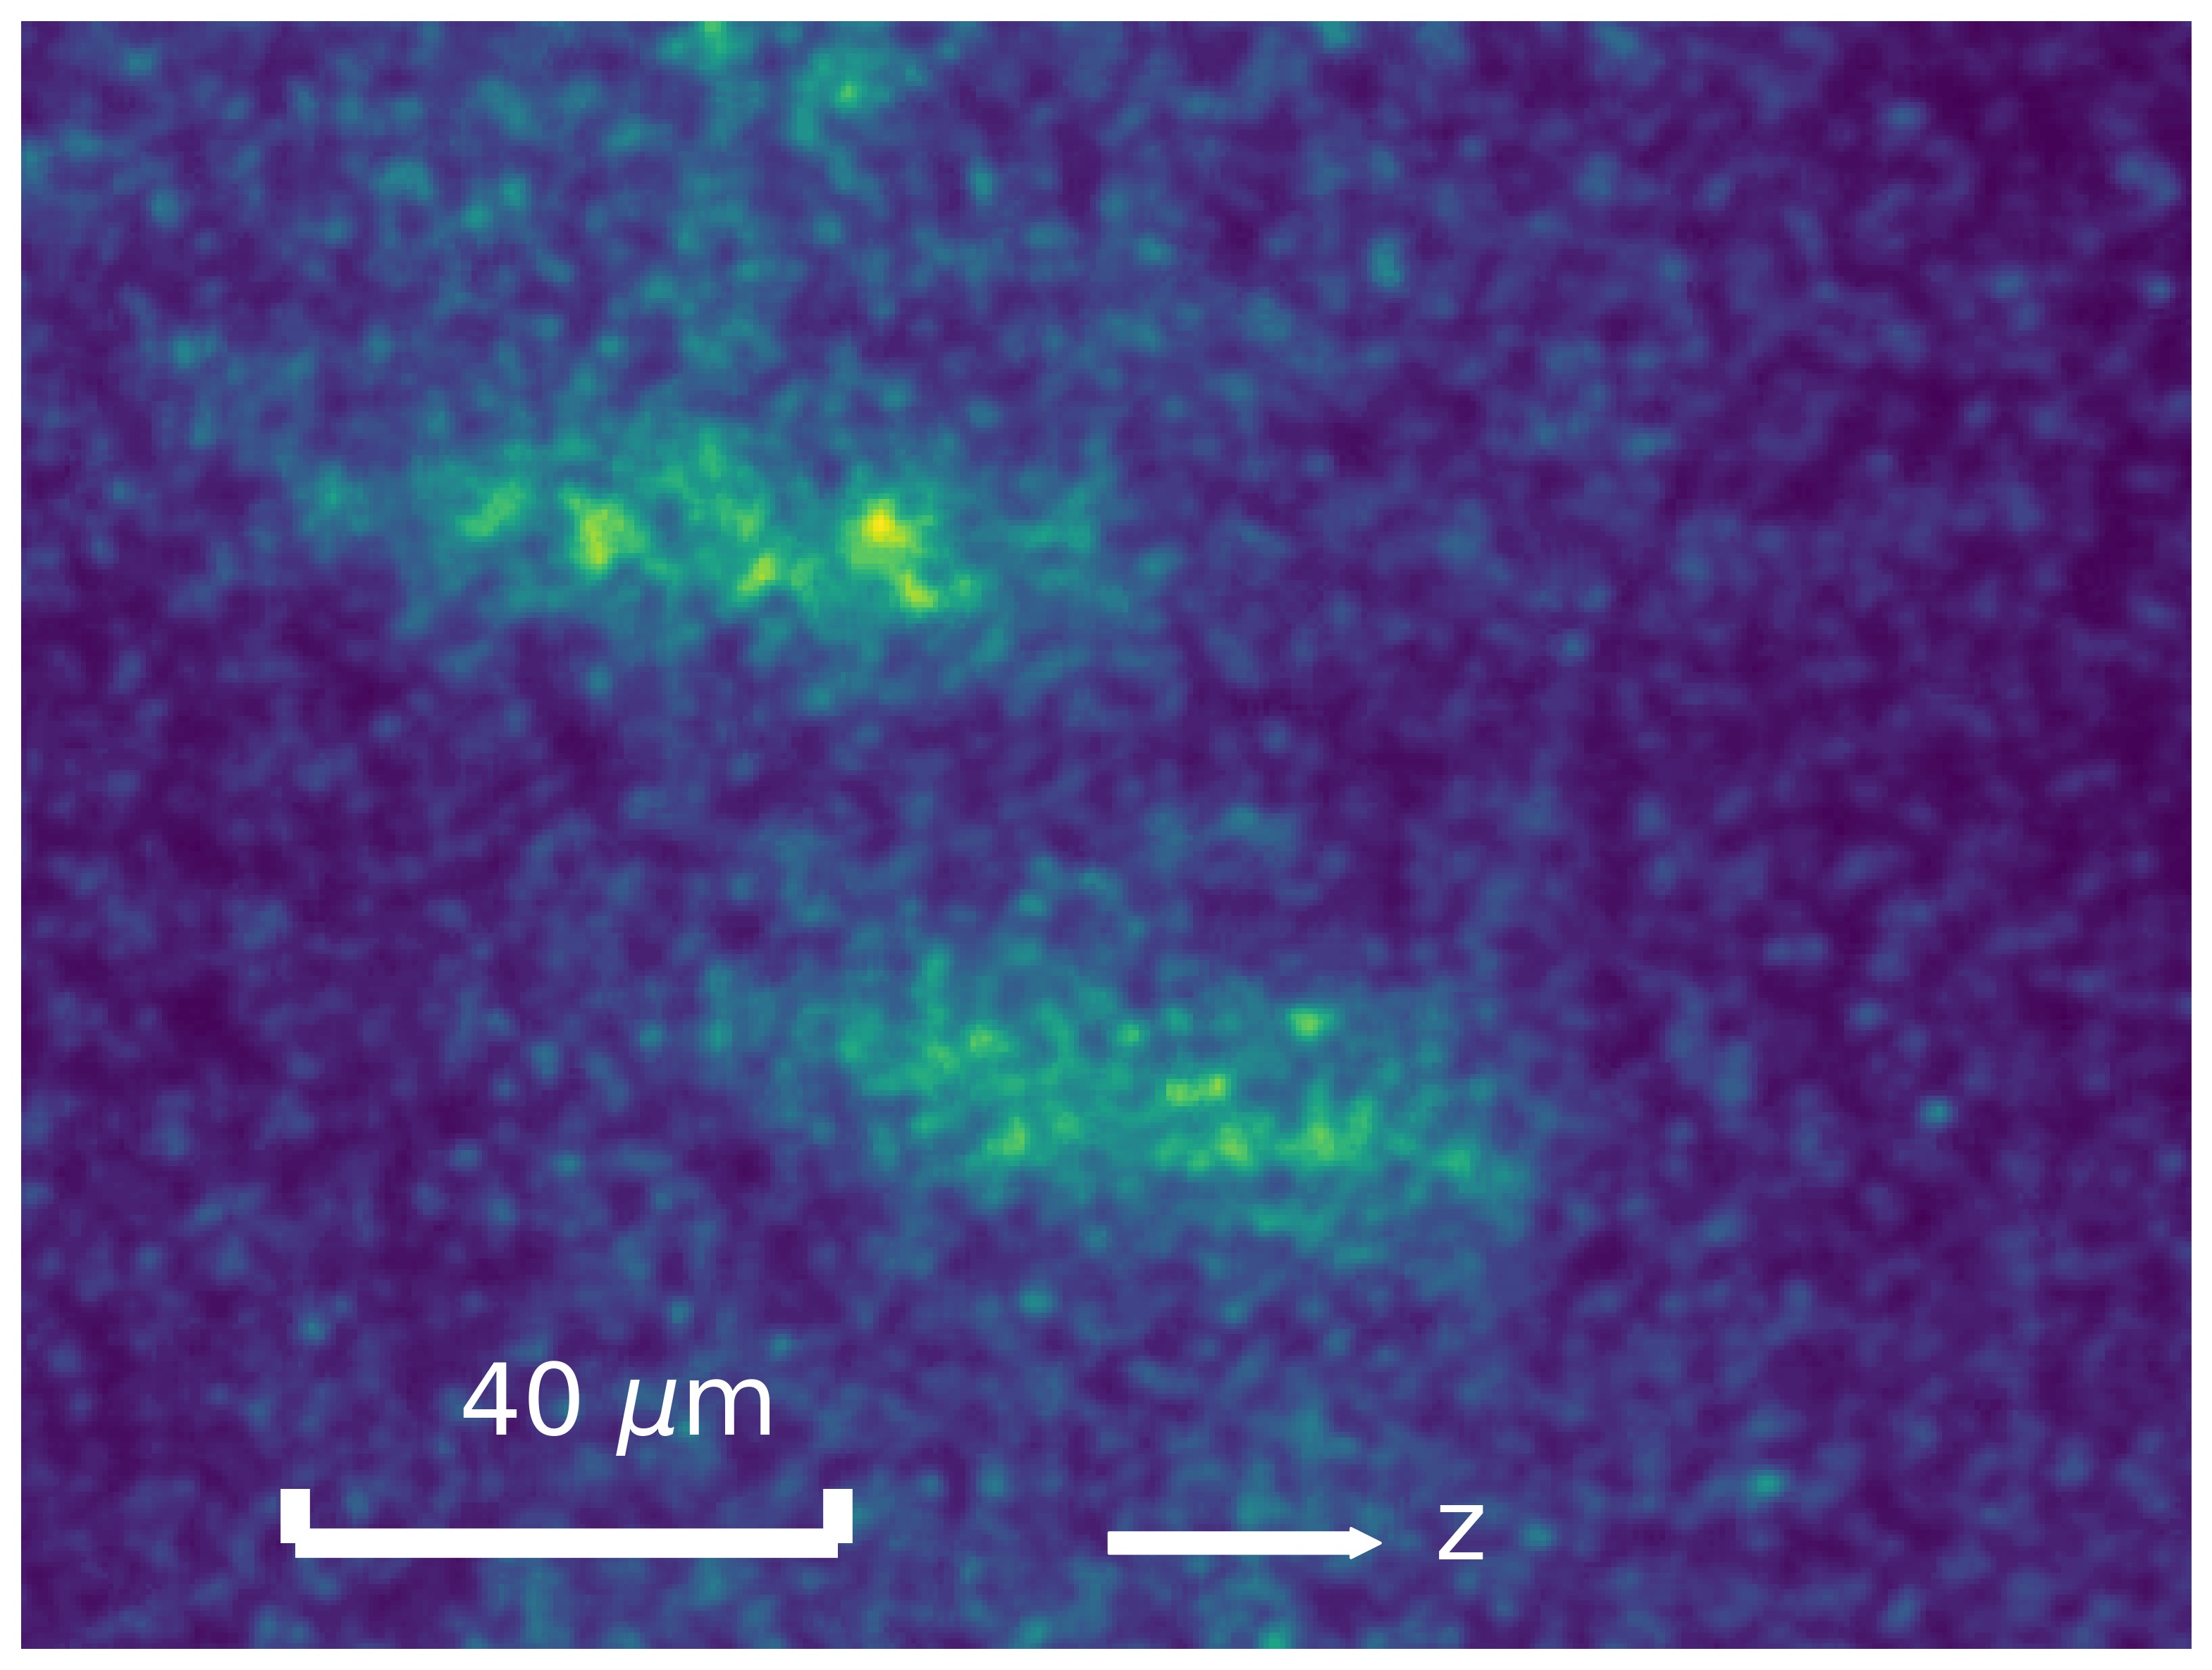
\includegraphics[width = 0.6\columnwidth]{./methods/figure/4_2D.jpg}
		\caption{手順4. でのイオン捕獲画像}
		\label{fig:4_2D}
	\end{center}
	\end{minipage}
	\begin{minipage}{0.48\linewidth}
		\begin{center}
			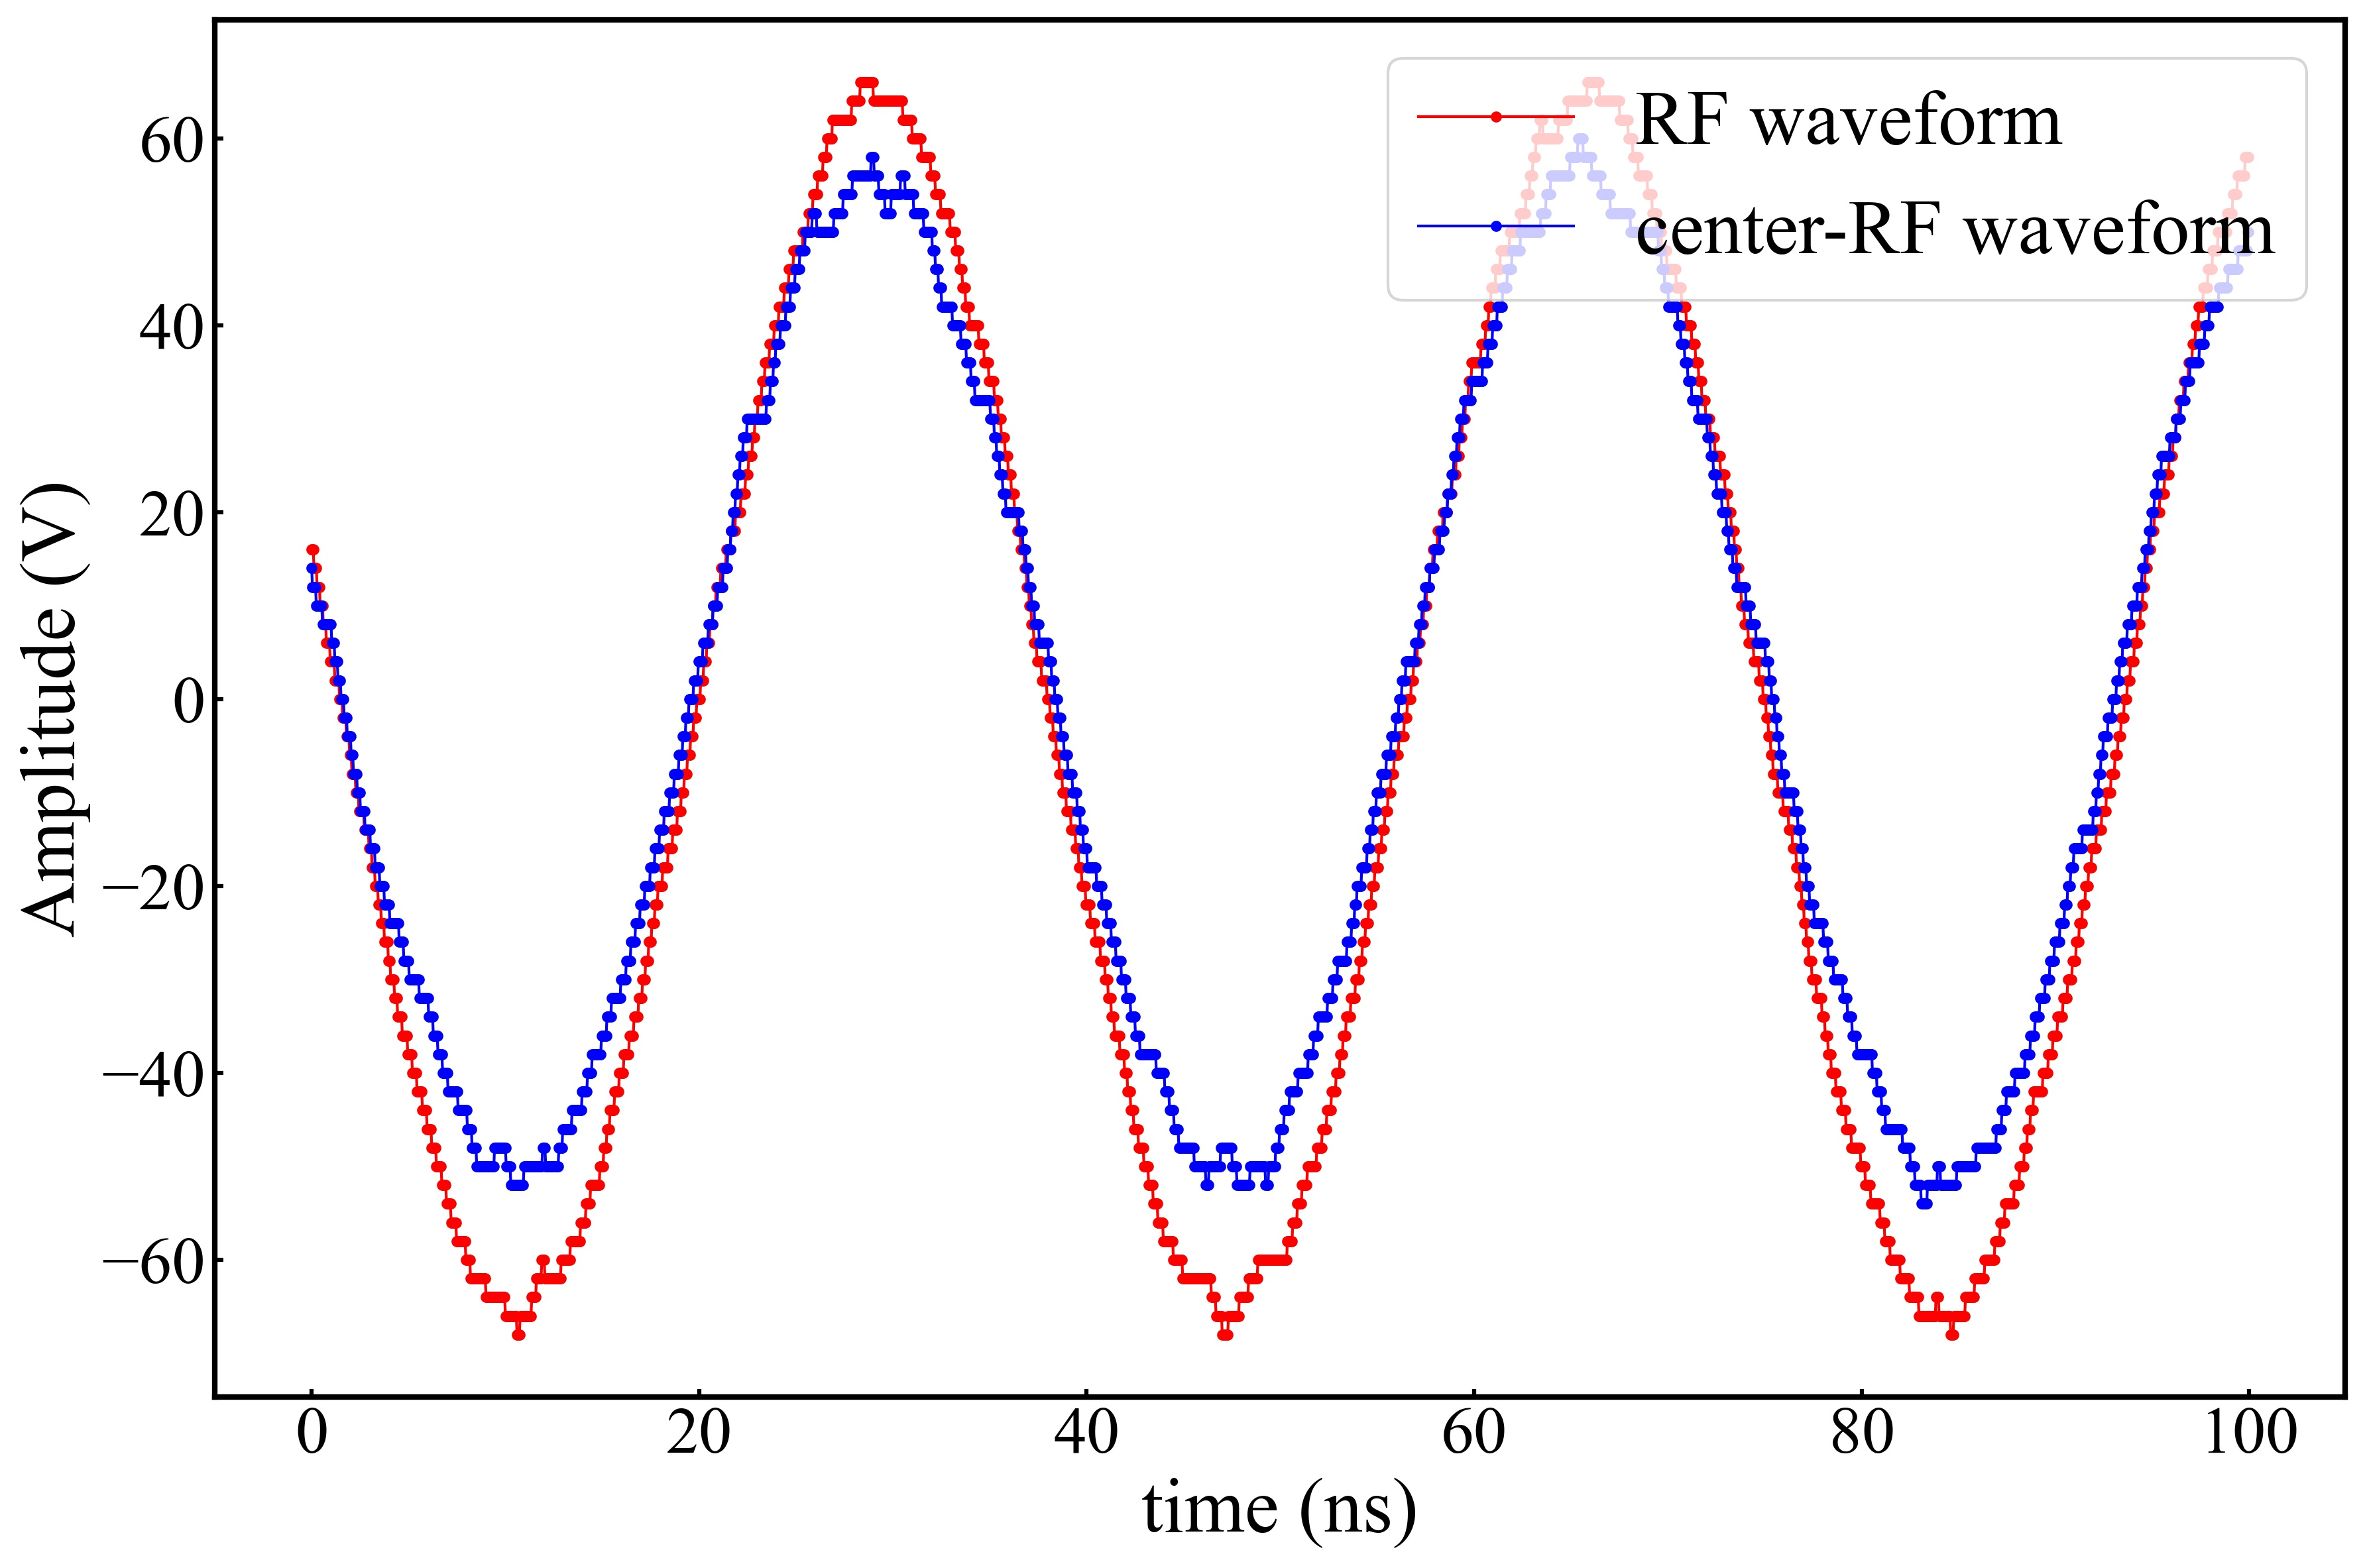
\includegraphics[width = 0.9\columnwidth]{./methods/figure/4_2D_wave.jpg}
			\caption{手順4. におけるrf電圧とcenter-rf電圧の関係}
			\label{fig:4_2D_wave}
		\end{center}
	\end{minipage}
\end{figure}

このとき,$R=0.86$となっている.マイクロメータの目盛は\Tb{3_2D}から変更は行っていない.\Fig{4_2D}より,クラウド状でイオンが二列に捕獲されることが確認できる.また,center電極に印加する電圧を$V_{\rm center} = 0.335$ V,side1電極に印加するdc電圧を$V_{\rm side1} = 0.383$ Vに変更している.

\item 最後にcenter-rf電圧の振幅を180 mVppに設定する.\Fig{5_2D}にイオン捕獲画像を示し,\Fig{5_2D_wave}にrf電圧とcenter-rf電圧の関係を示している.

\begin{figure}[h]
	\begin{minipage}{0.48\linewidth}
	\begin{center}
		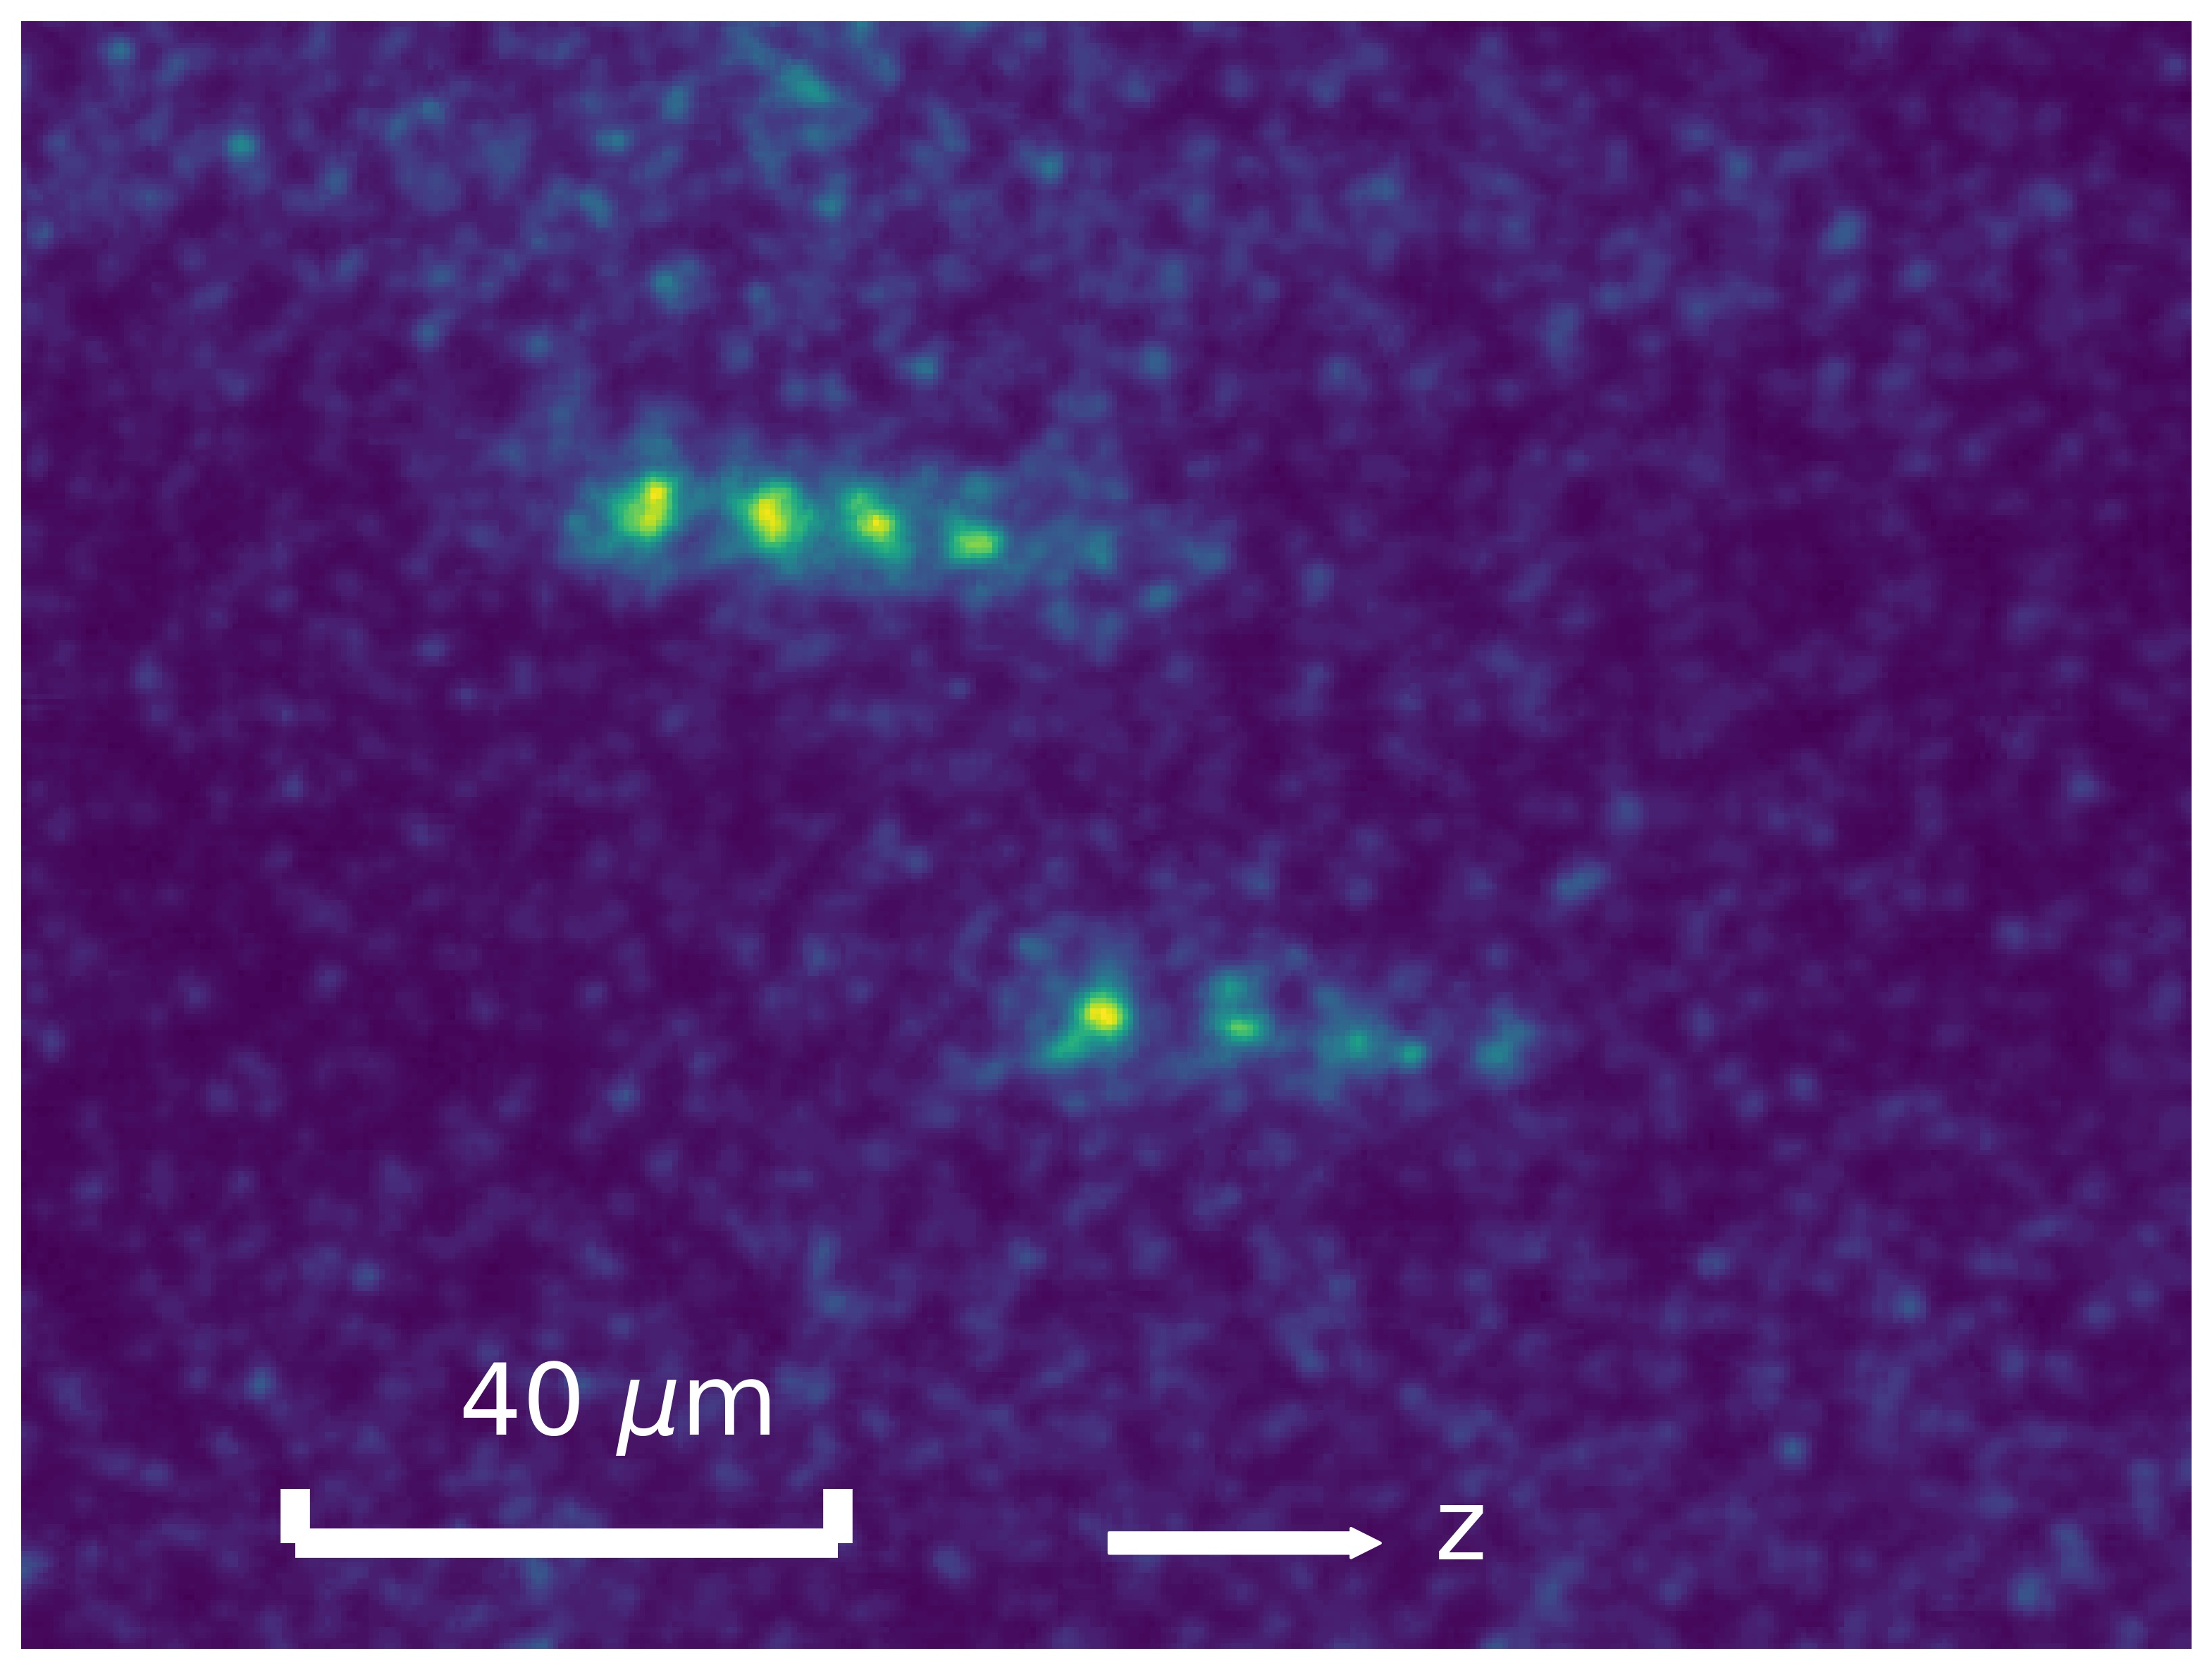
\includegraphics[width = 0.6\columnwidth]{./methods/figure/5_2D.jpg}
		\caption{手順5. でのイオン捕獲画像}
		\label{fig:5_2D}
	\end{center}
	\end{minipage}
	\begin{minipage}{0.48\linewidth}
		\begin{center}
			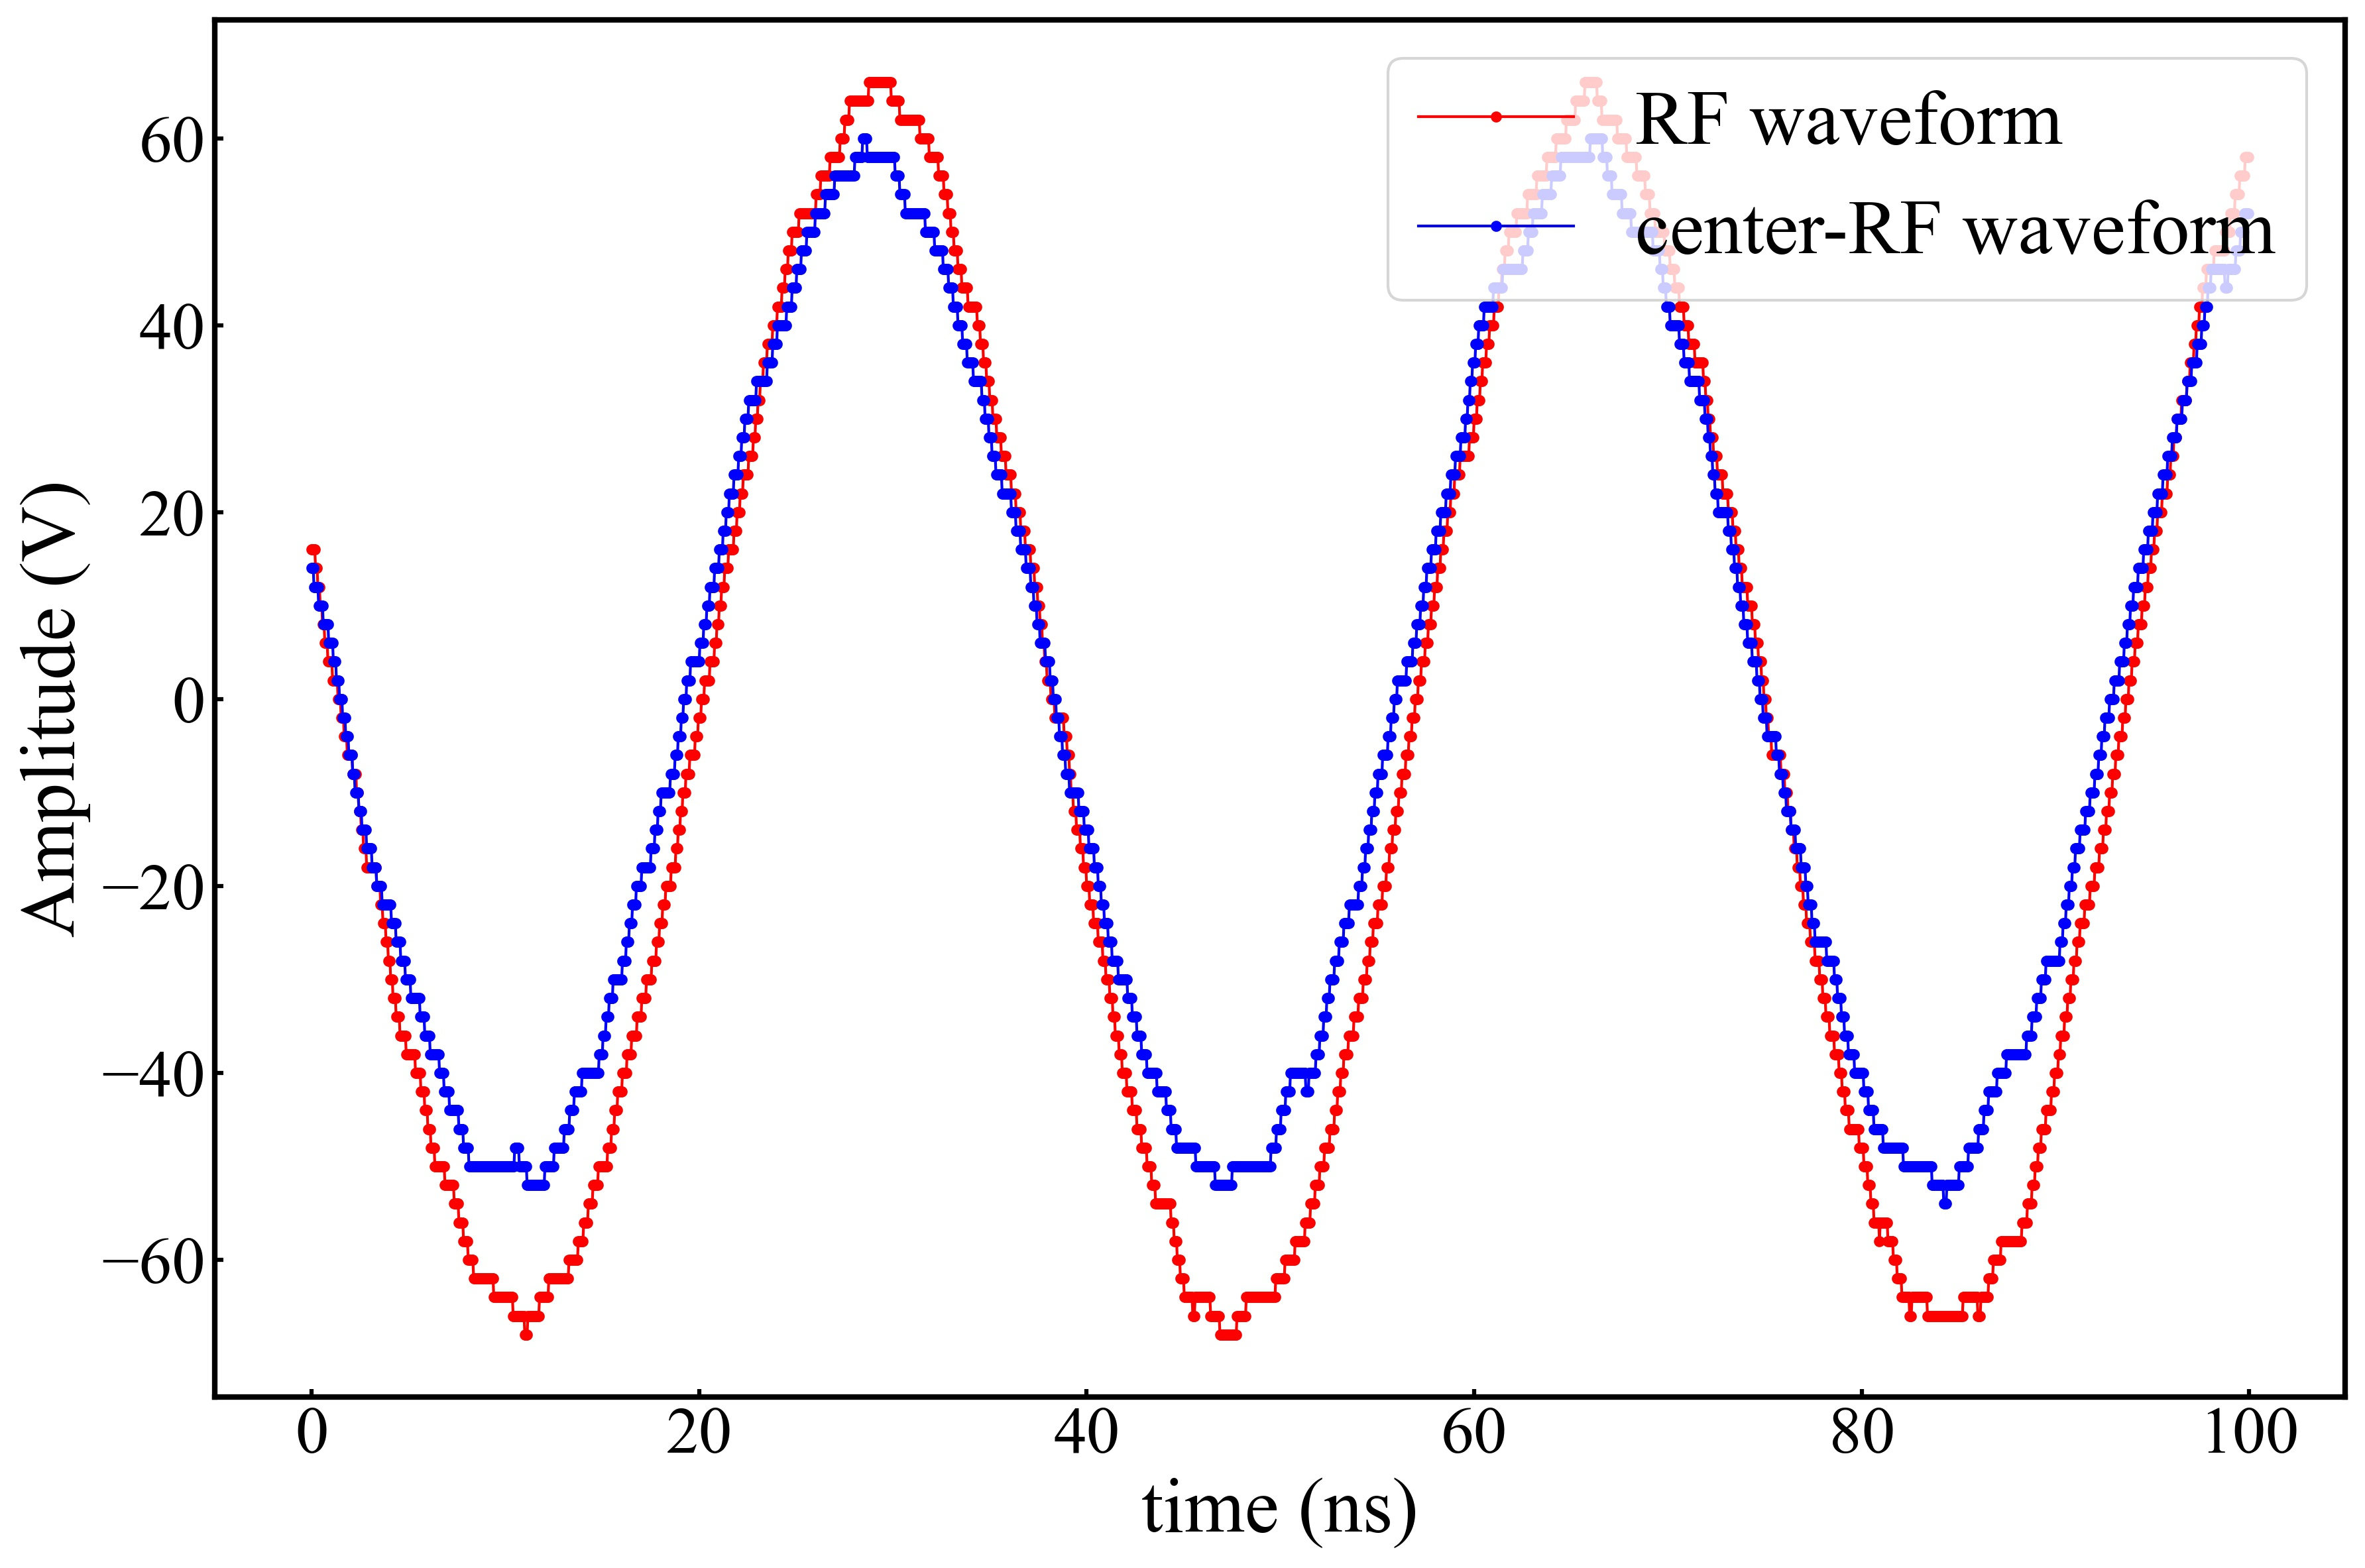
\includegraphics[width = 0.9\columnwidth]{./methods/figure/5_2D_wave.jpg}
			\caption{手順5. におけるrf電圧とcenter-rf電圧の関係}
			\label{fig:5_2D_wave}
		\end{center}
	\end{minipage}
\end{figure}

このとき,$R=0.91$となっている.このとき,$V_{\rm center} = 0.225$ Vにcenter電極に印加する電圧を変化させることでイオンの結晶化が観測されている.

\end{enumerate}

\clearpage

\section{永年周波数の測定方法} \label{MeasSecFreq_Method}
プレーナートラップ上の電場を直接的に測定することはできない.単一イオンの捕獲位置におけるポテンシャルの概形を見積もり,電場の傾きの算出を行うため,単一イオンの永年周波数の測定システムの開発を行った.dc電極にac信号を重畳させることでイオンに共鳴現象を引き起こすことが可能であり,共鳴時にはイオンの蛍光量が減少し,また,その振幅が拡がることが画像から確認することができる.本実験では,\Fig{MeasSec_System}に示すF.G.2から出力するac信号をmiddle1電極に重畳し周波数掃引を行ったときのイオンの振幅の周波数特性を取得し,ローレンツ分布関数によるフィッティングを行うことで永年周波数の測定を行った.また,イオンの振幅を計測するにあたり,S/N比を向上させるため積算回数を15回としている.

\begin{figure}[h]
	\centering
	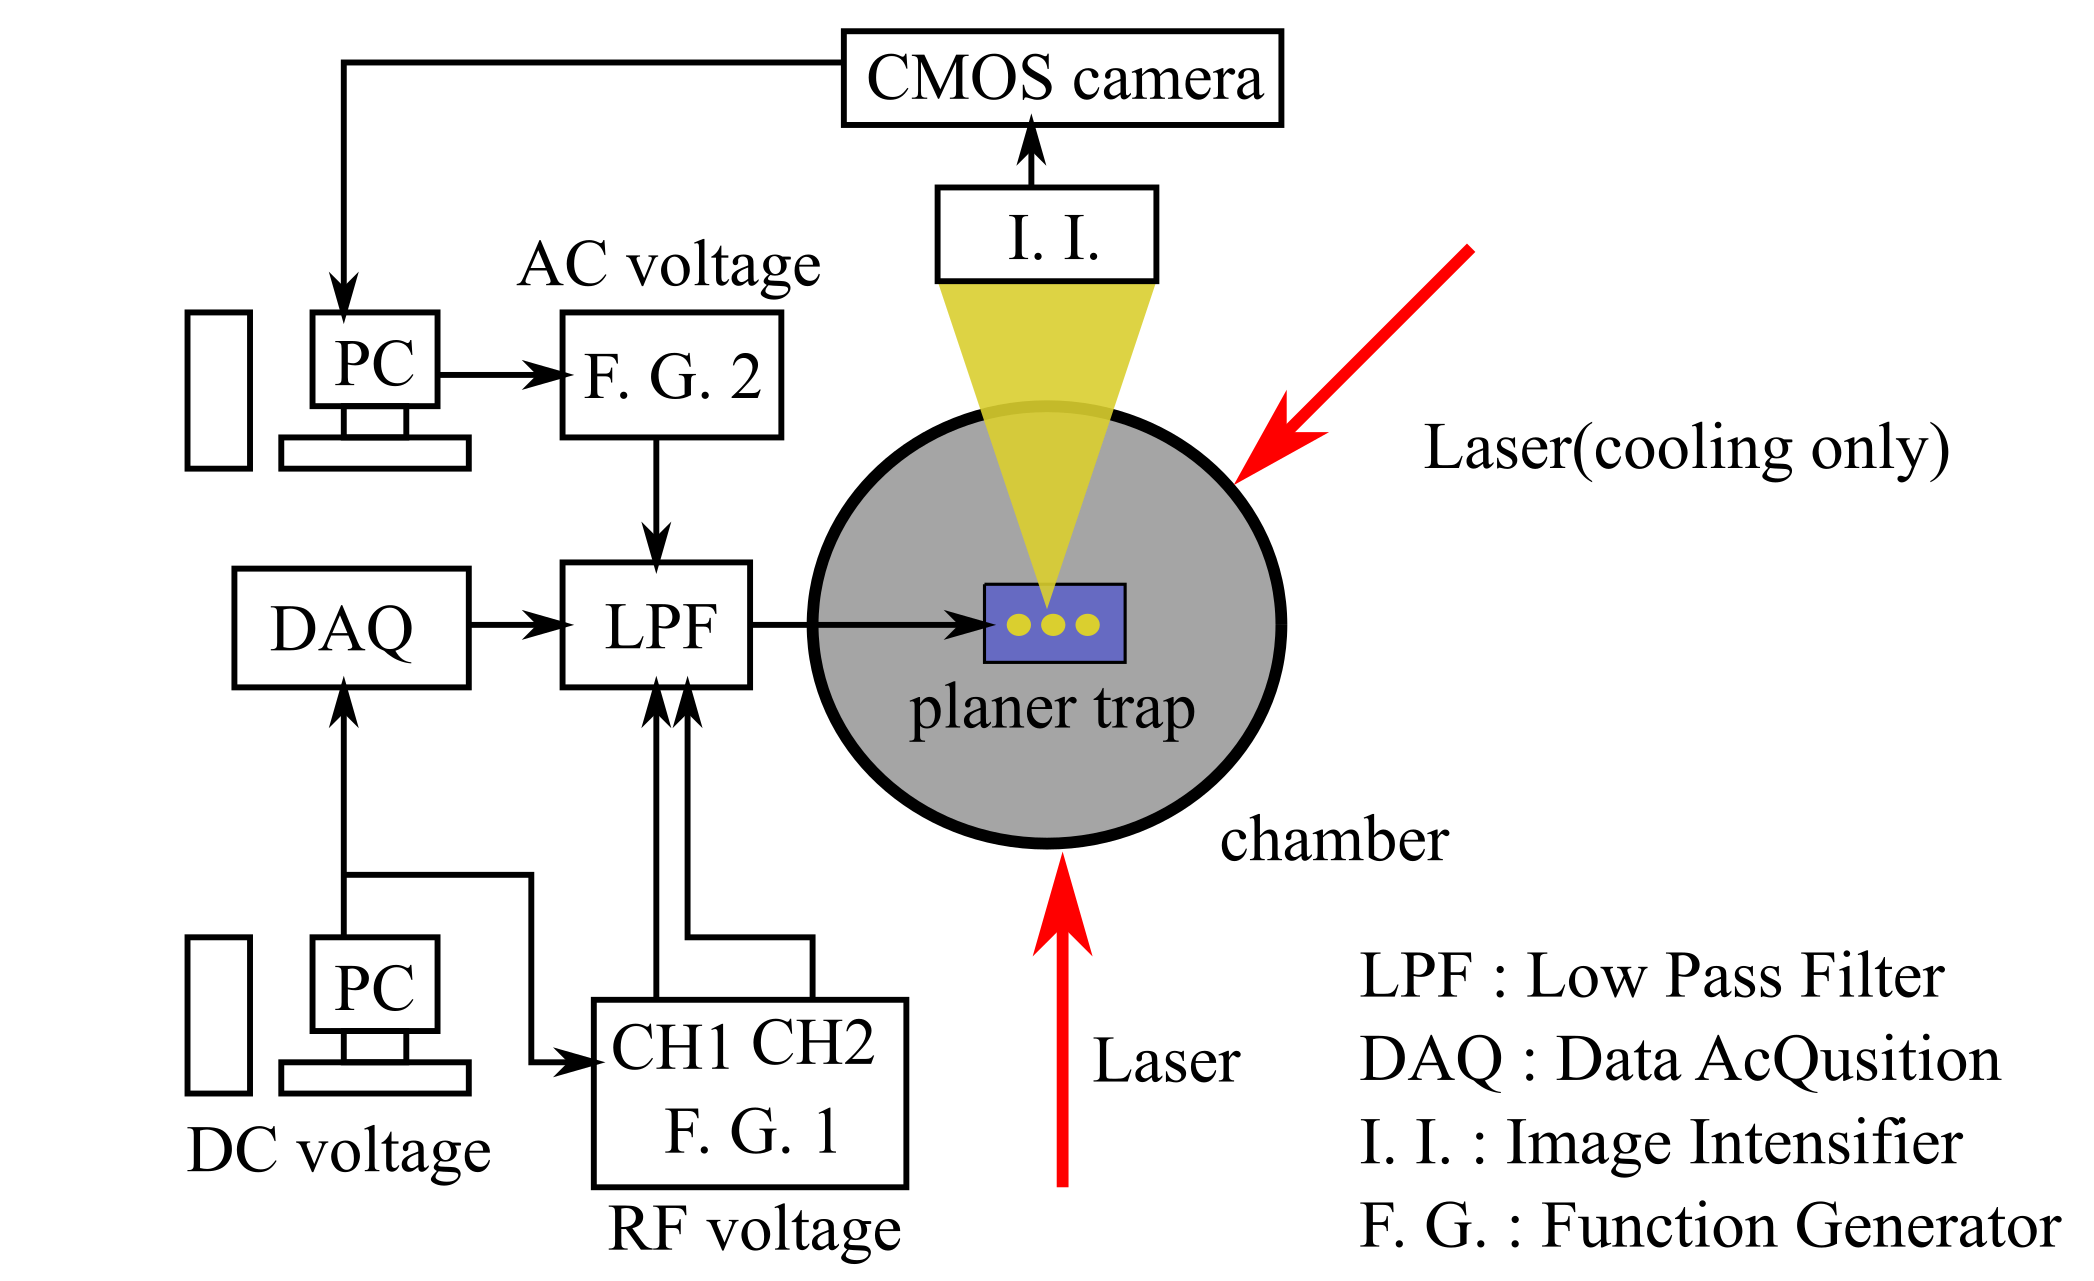
\includegraphics[width = 0.6\linewidth]{./methods/figure/SecularFreqMeasSetup.png}
	\caption{永年周波数測定のための実験系}
	\label{fig:MeasSec_System}
\end{figure}

\Fig{example_off_resonance}と\Fig{example_resonance}に非共鳴時と共鳴時(z方向)のイオンの振幅の様子を示す.

\begin{figure}[h]
		\begin{minipage}{0.48\linewidth}
			\centering
			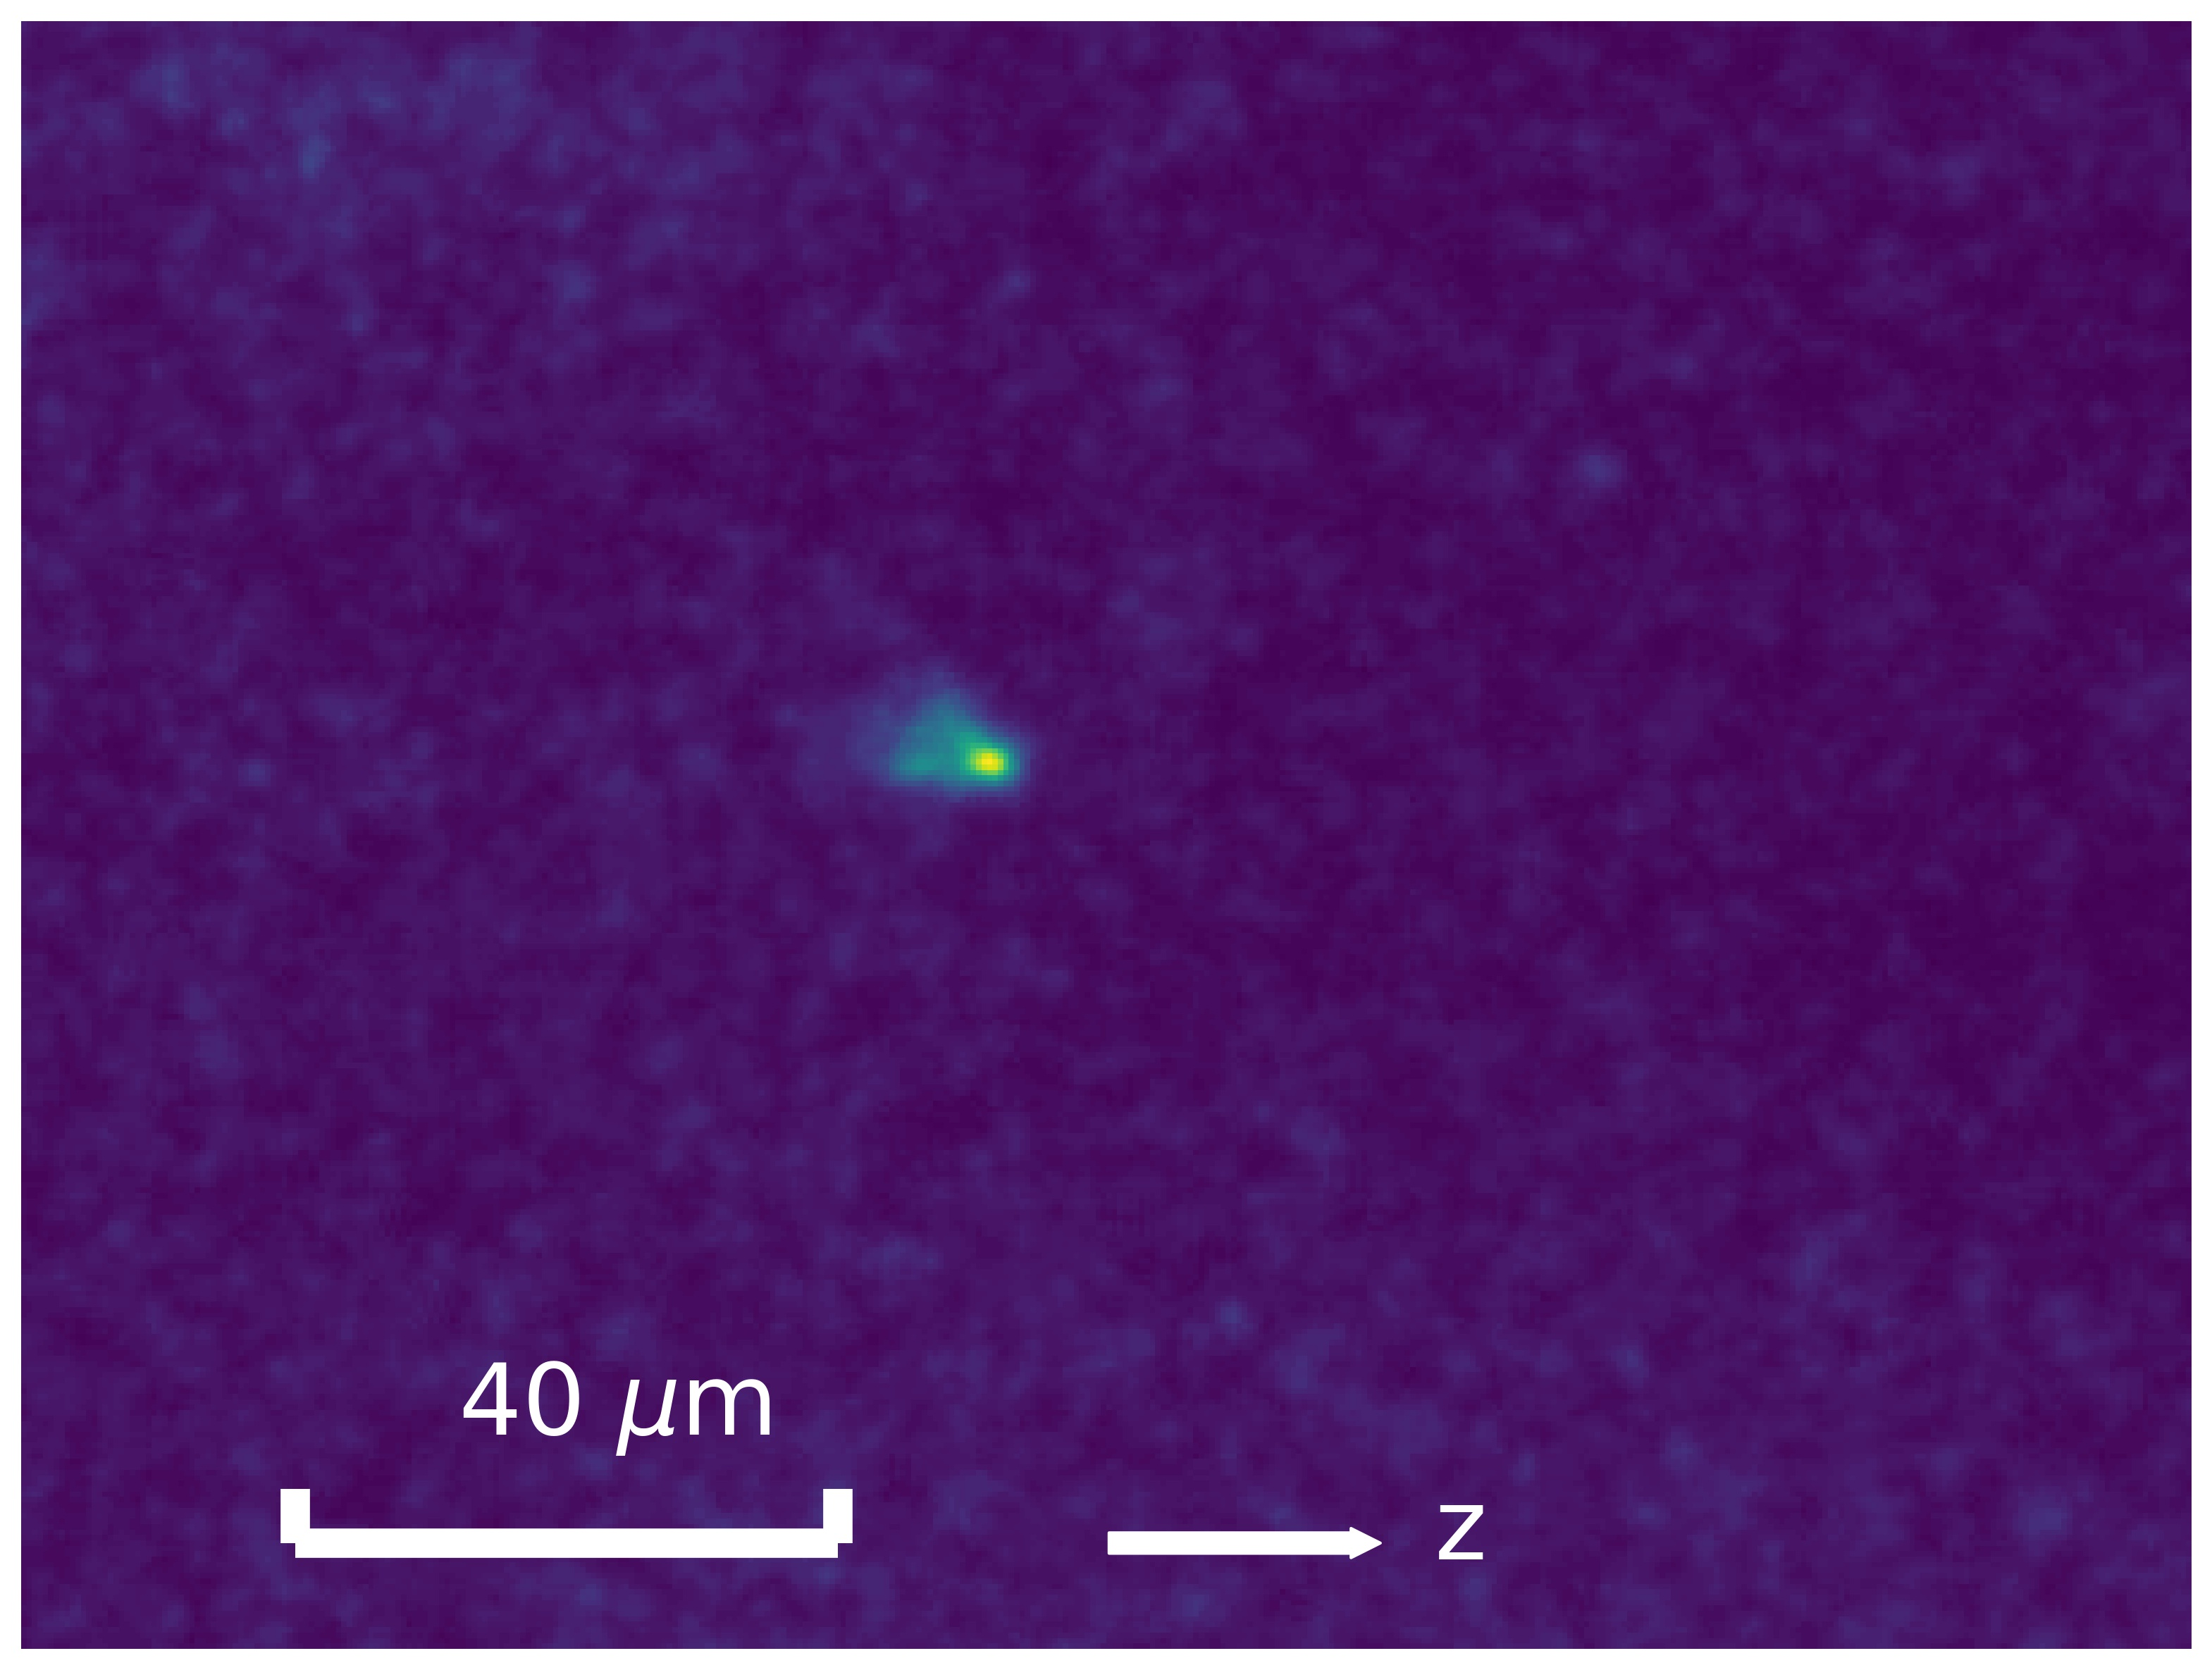
\includegraphics[width = 0.6\columnwidth]{./methods/figure/off_resonance.jpg}
			\caption{非共鳴時のイオンの捕獲画像}
			\label{fig:example_off_resonance}
		\end{minipage}
		\begin{minipage}{0.48\linewidth}
			\centering
			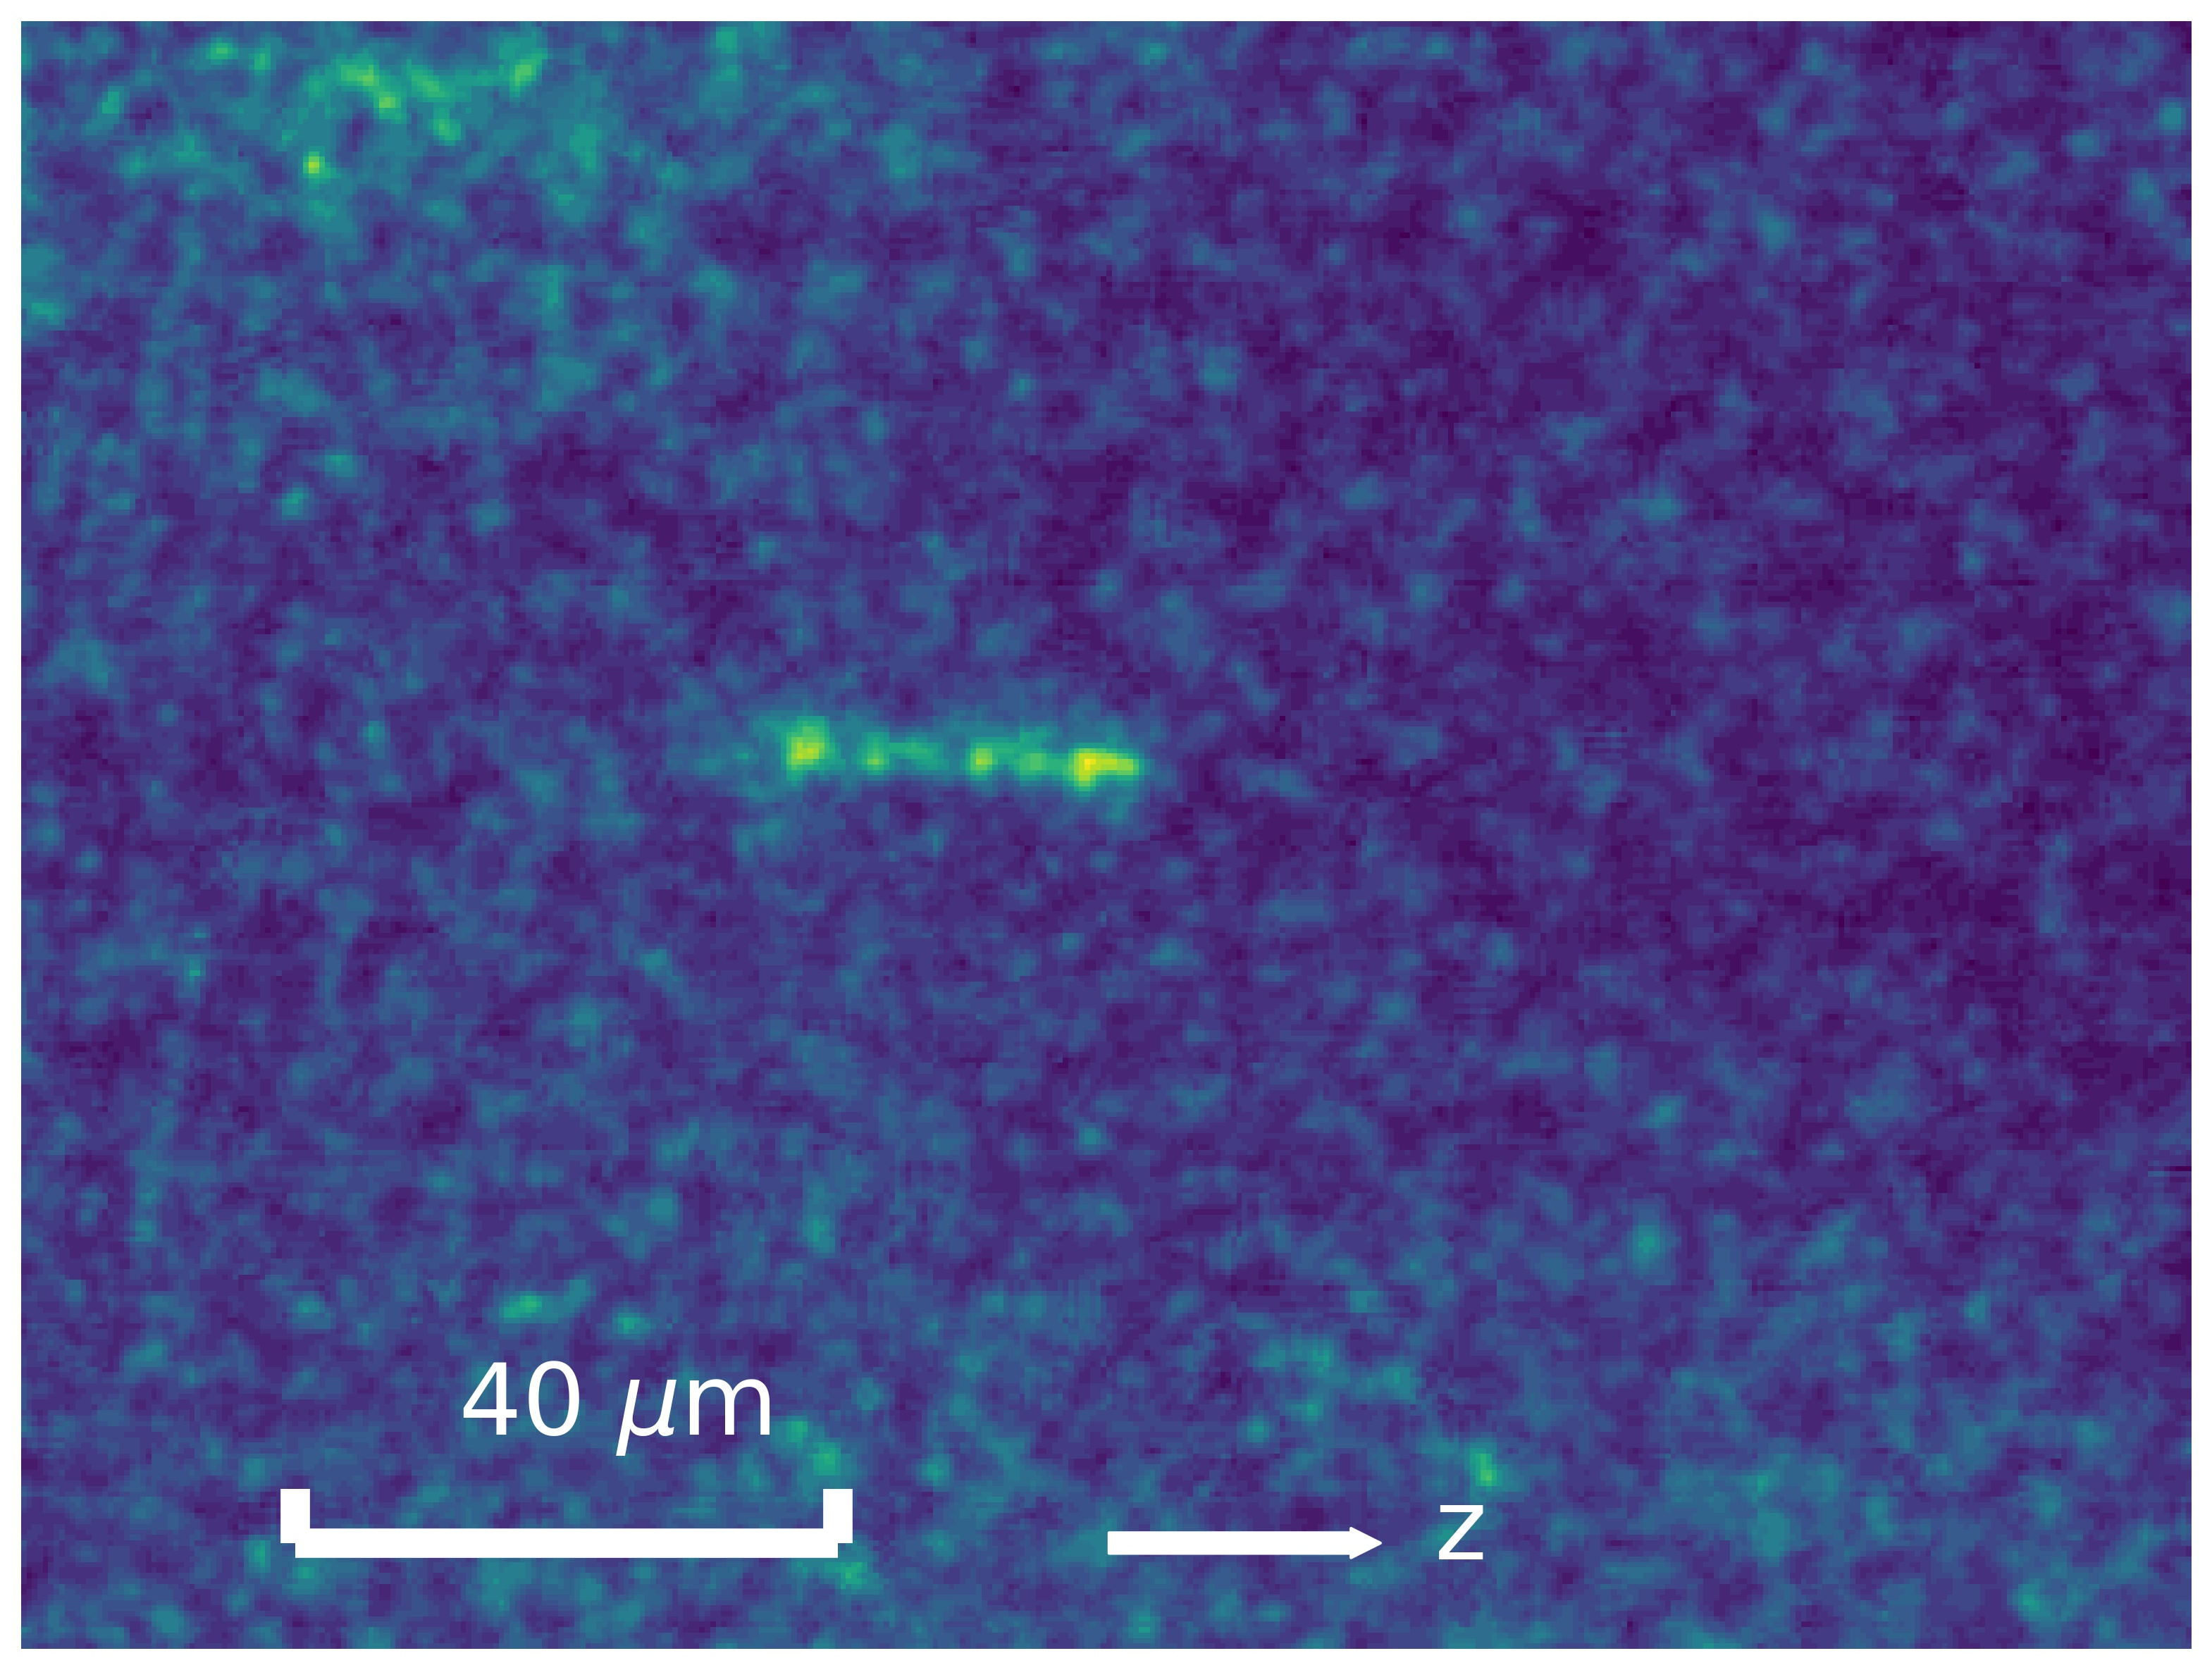
\includegraphics[width = 0.6\columnwidth]{./methods/figure/resonance.jpg}
			\caption{共鳴時のイオンの捕獲画像}
			\label{fig:example_resonance}
		\end{minipage}
\end{figure}

\Fig{example_resonance}より共鳴時にイオンの振幅が拡がることが分かる.

\clearpage

ここで,イオンの振幅は蛍光強度の最大値$I_{\rm max}$としたときの$I_{\rm max}/2$における蛍光強度の幅をイオンの振幅としてみなしている.非共鳴時(\Fig{example_off_resonance})と共鳴時(\Fig{example_resonance})のz軸に沿ったイオンの蛍光強度のプロファイルを\Fig{example_off_resonance_Amp}と\Fig{example_resonance_Amp}に示す.

\begin{figure}[h]
	\begin{minipage}{0.5\linewidth}
		\begin{center}
			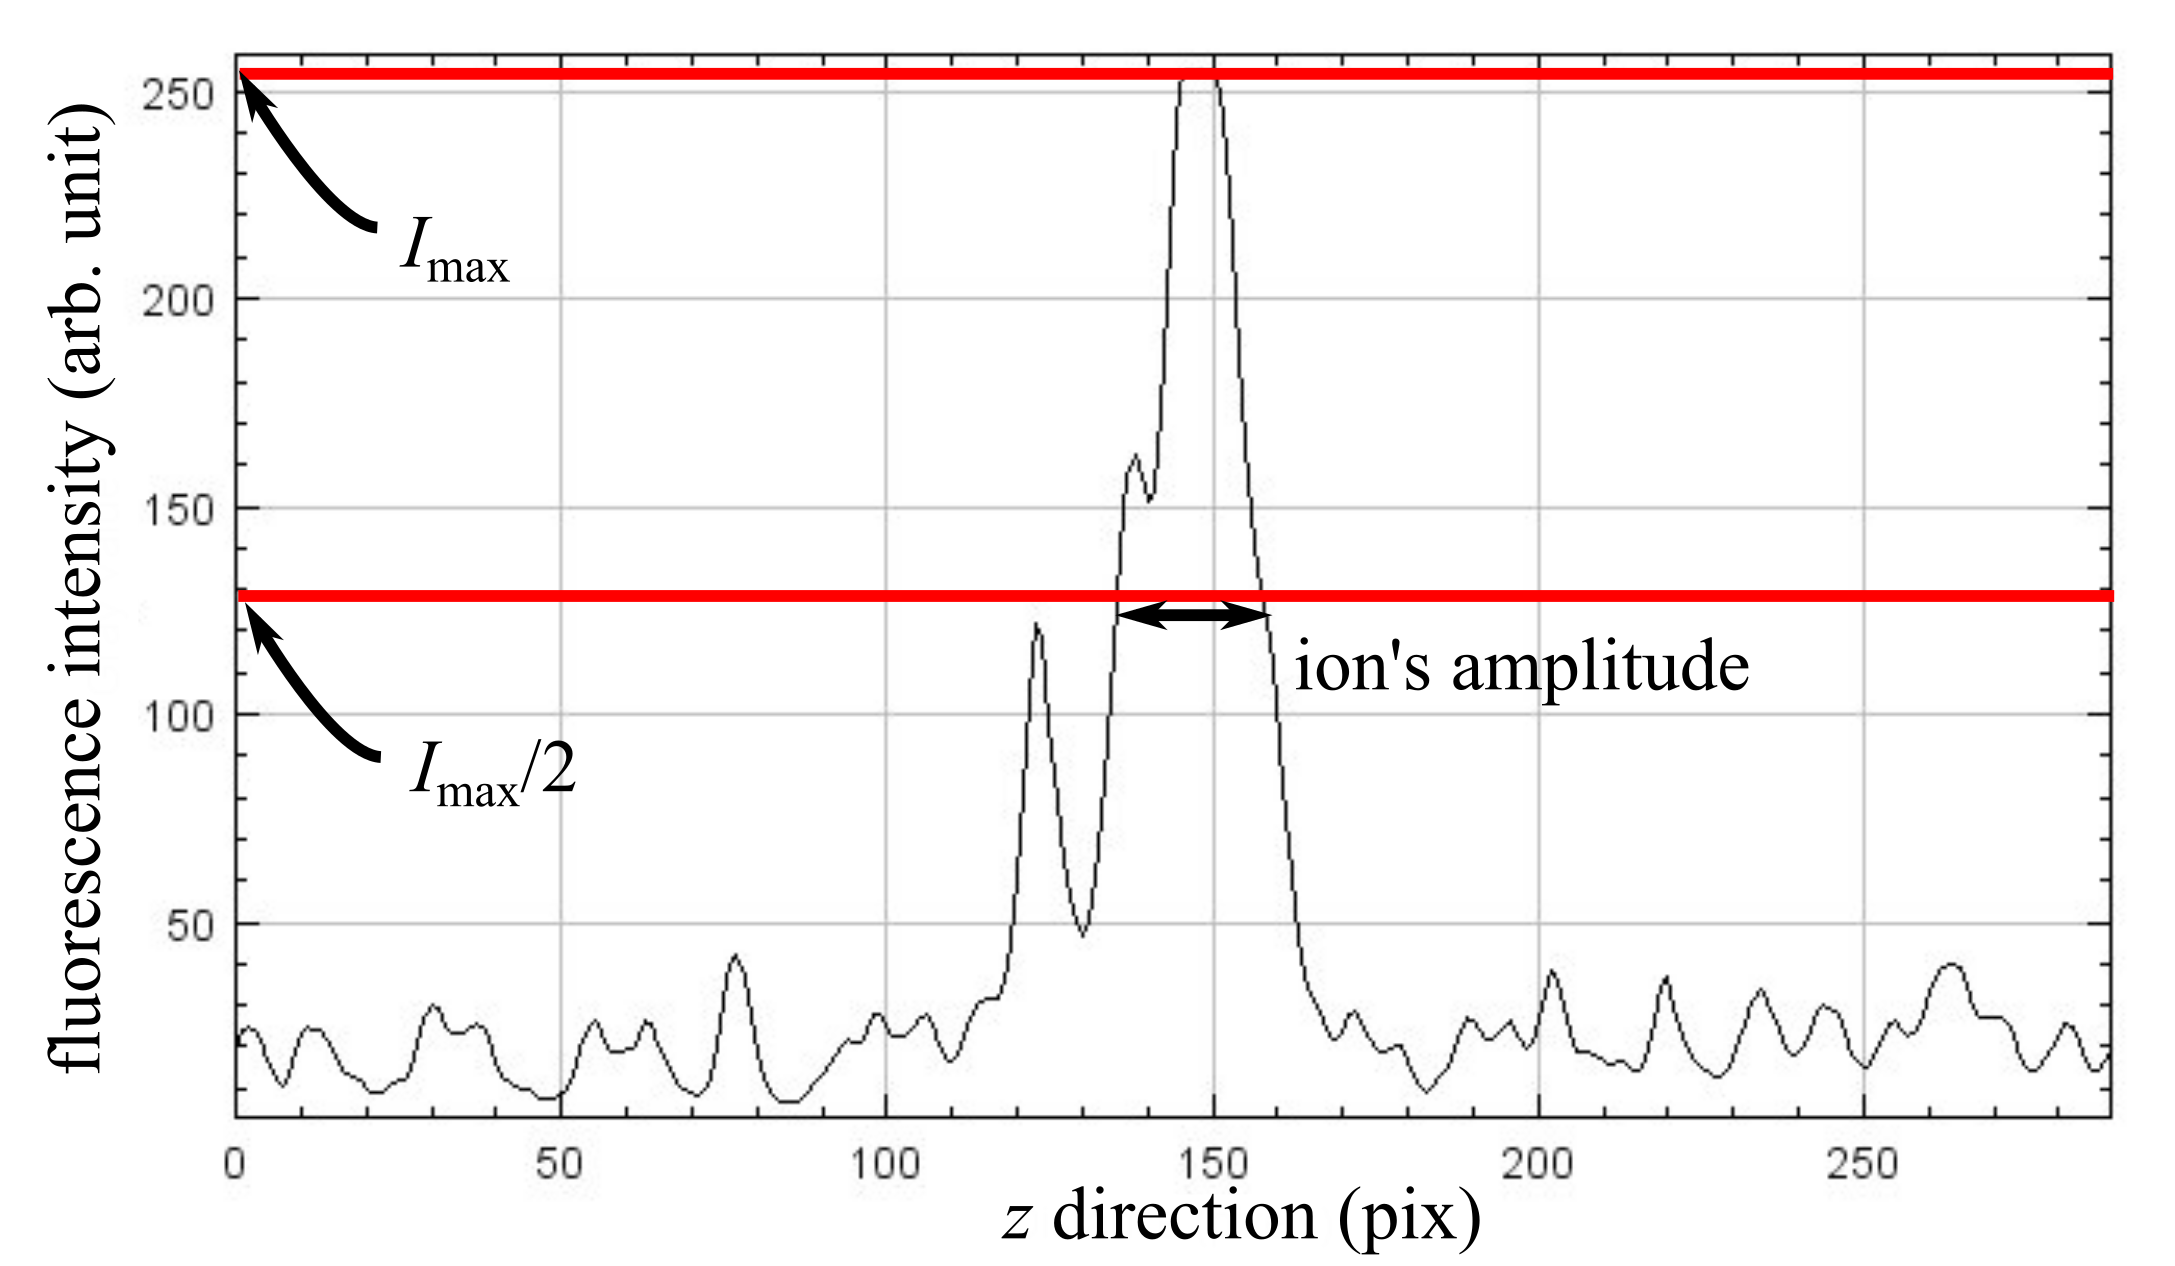
\includegraphics[width = 0.98\columnwidth]{./methods/figure/PlotOf_off_resonance.png}
			\caption{\Fig{example_off_resonance}におけるイオンの振幅}
			\label{fig:example_off_resonance_Amp}
		\end{center}
	\end{minipage}
	\begin{minipage}{0.5\linewidth}
		\begin{center}
			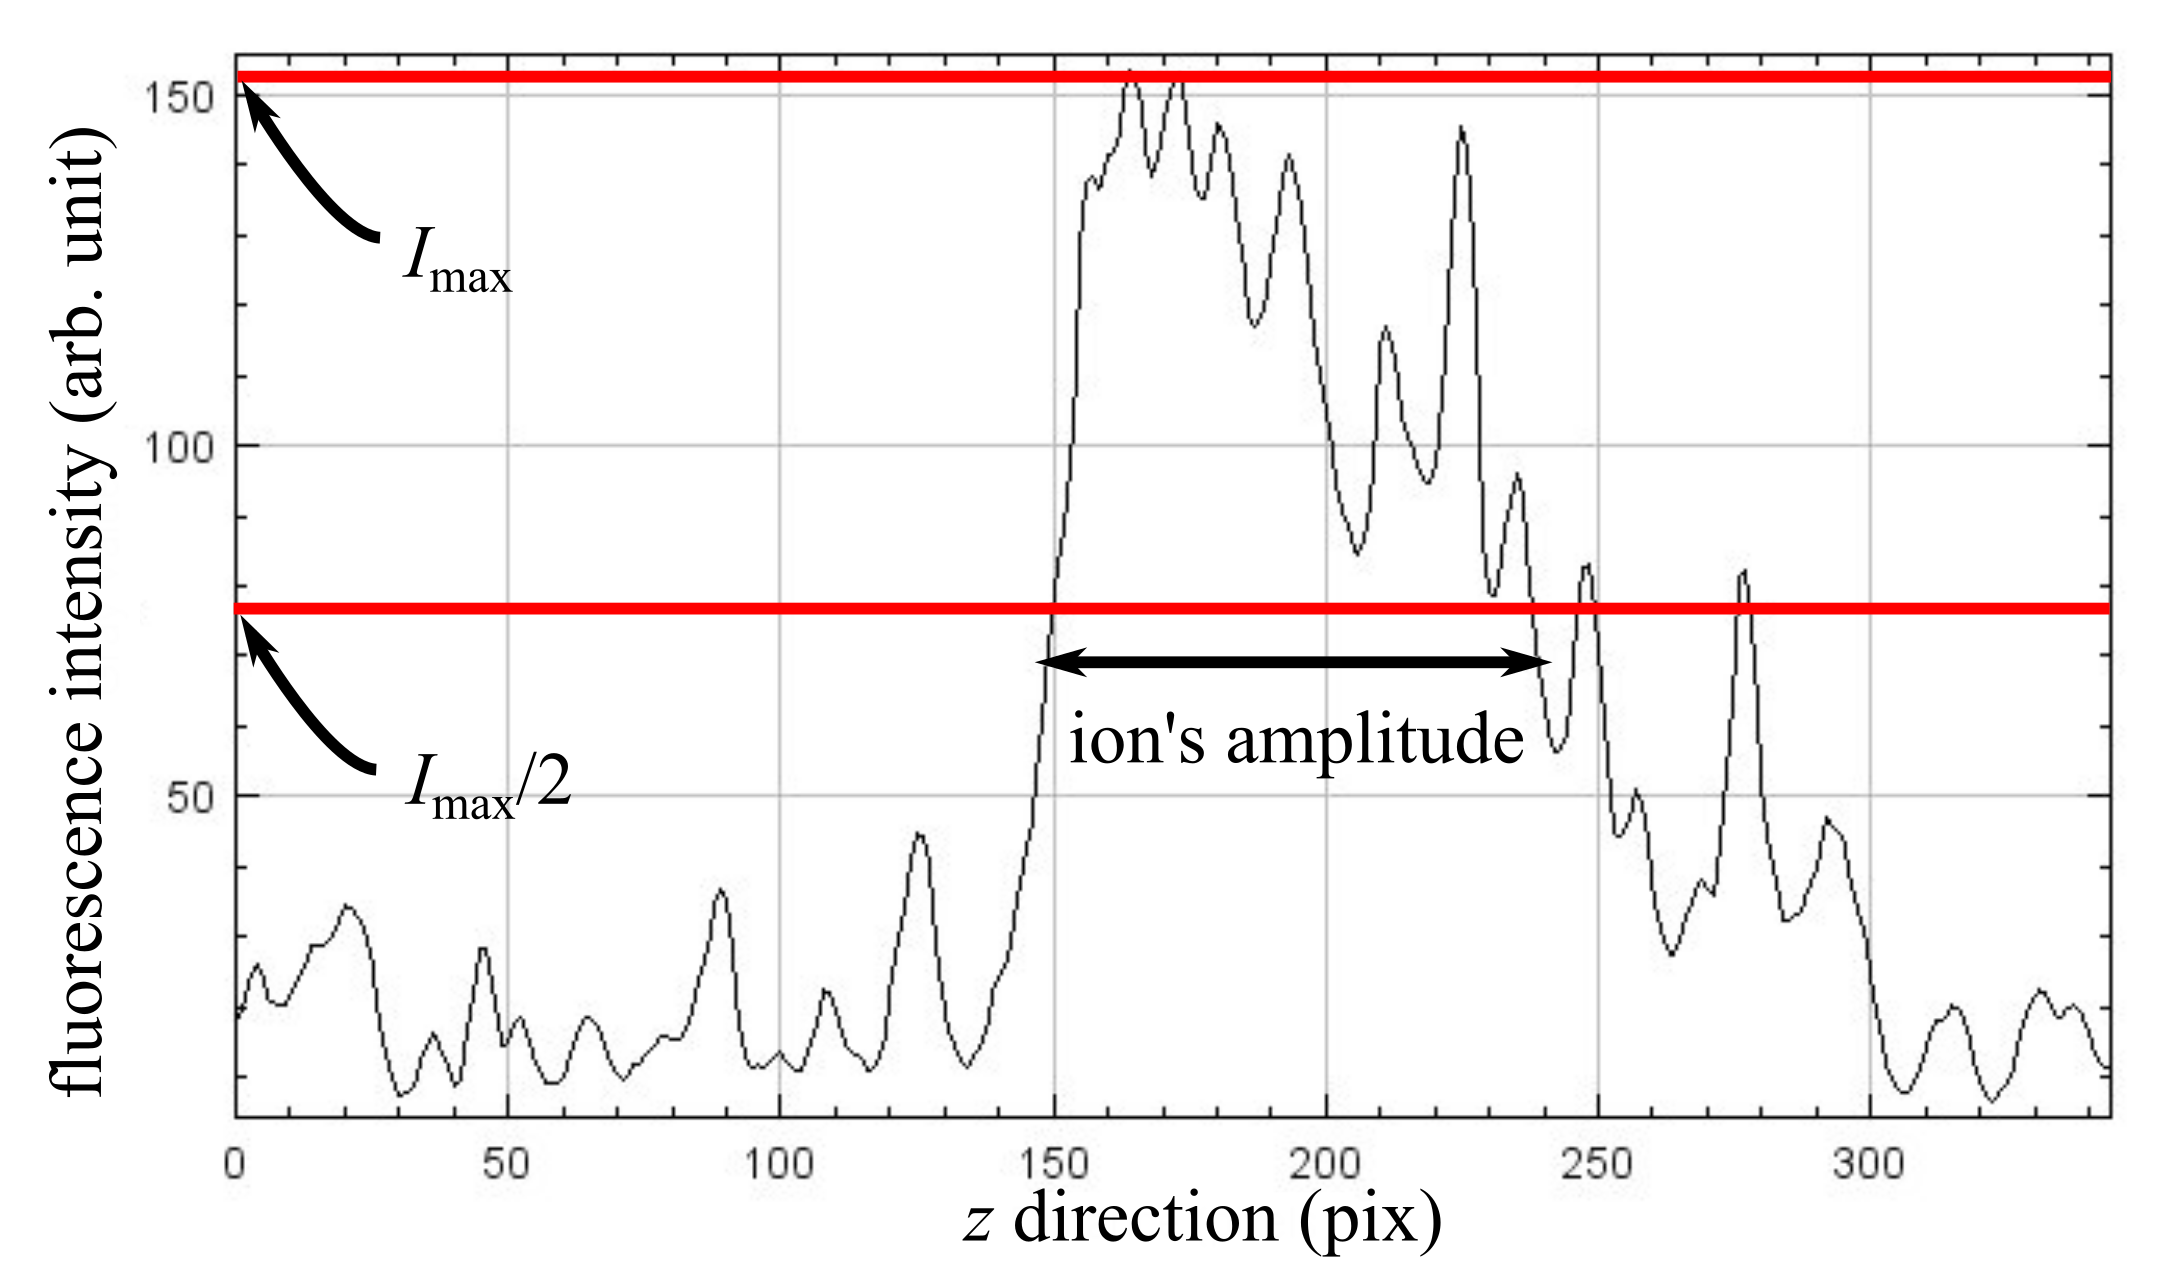
\includegraphics[width = 0.98\columnwidth]{./methods/figure/PlotOf_resonance.png}
			\caption{\Fig{example_resonance}におけるイオンの振幅}
			\label{fig:example_resonance_Amp}
		\end{center}
	\end{minipage}
\end{figure}

\Tb{dc_string}に示すdc電圧セットにおいて周波数掃引を行い取得したイオンの振幅の周波数特性と,そのフィッティング結果を\Fig{fitting_result}に示す.

\begin{figure}[h]
	\centering
		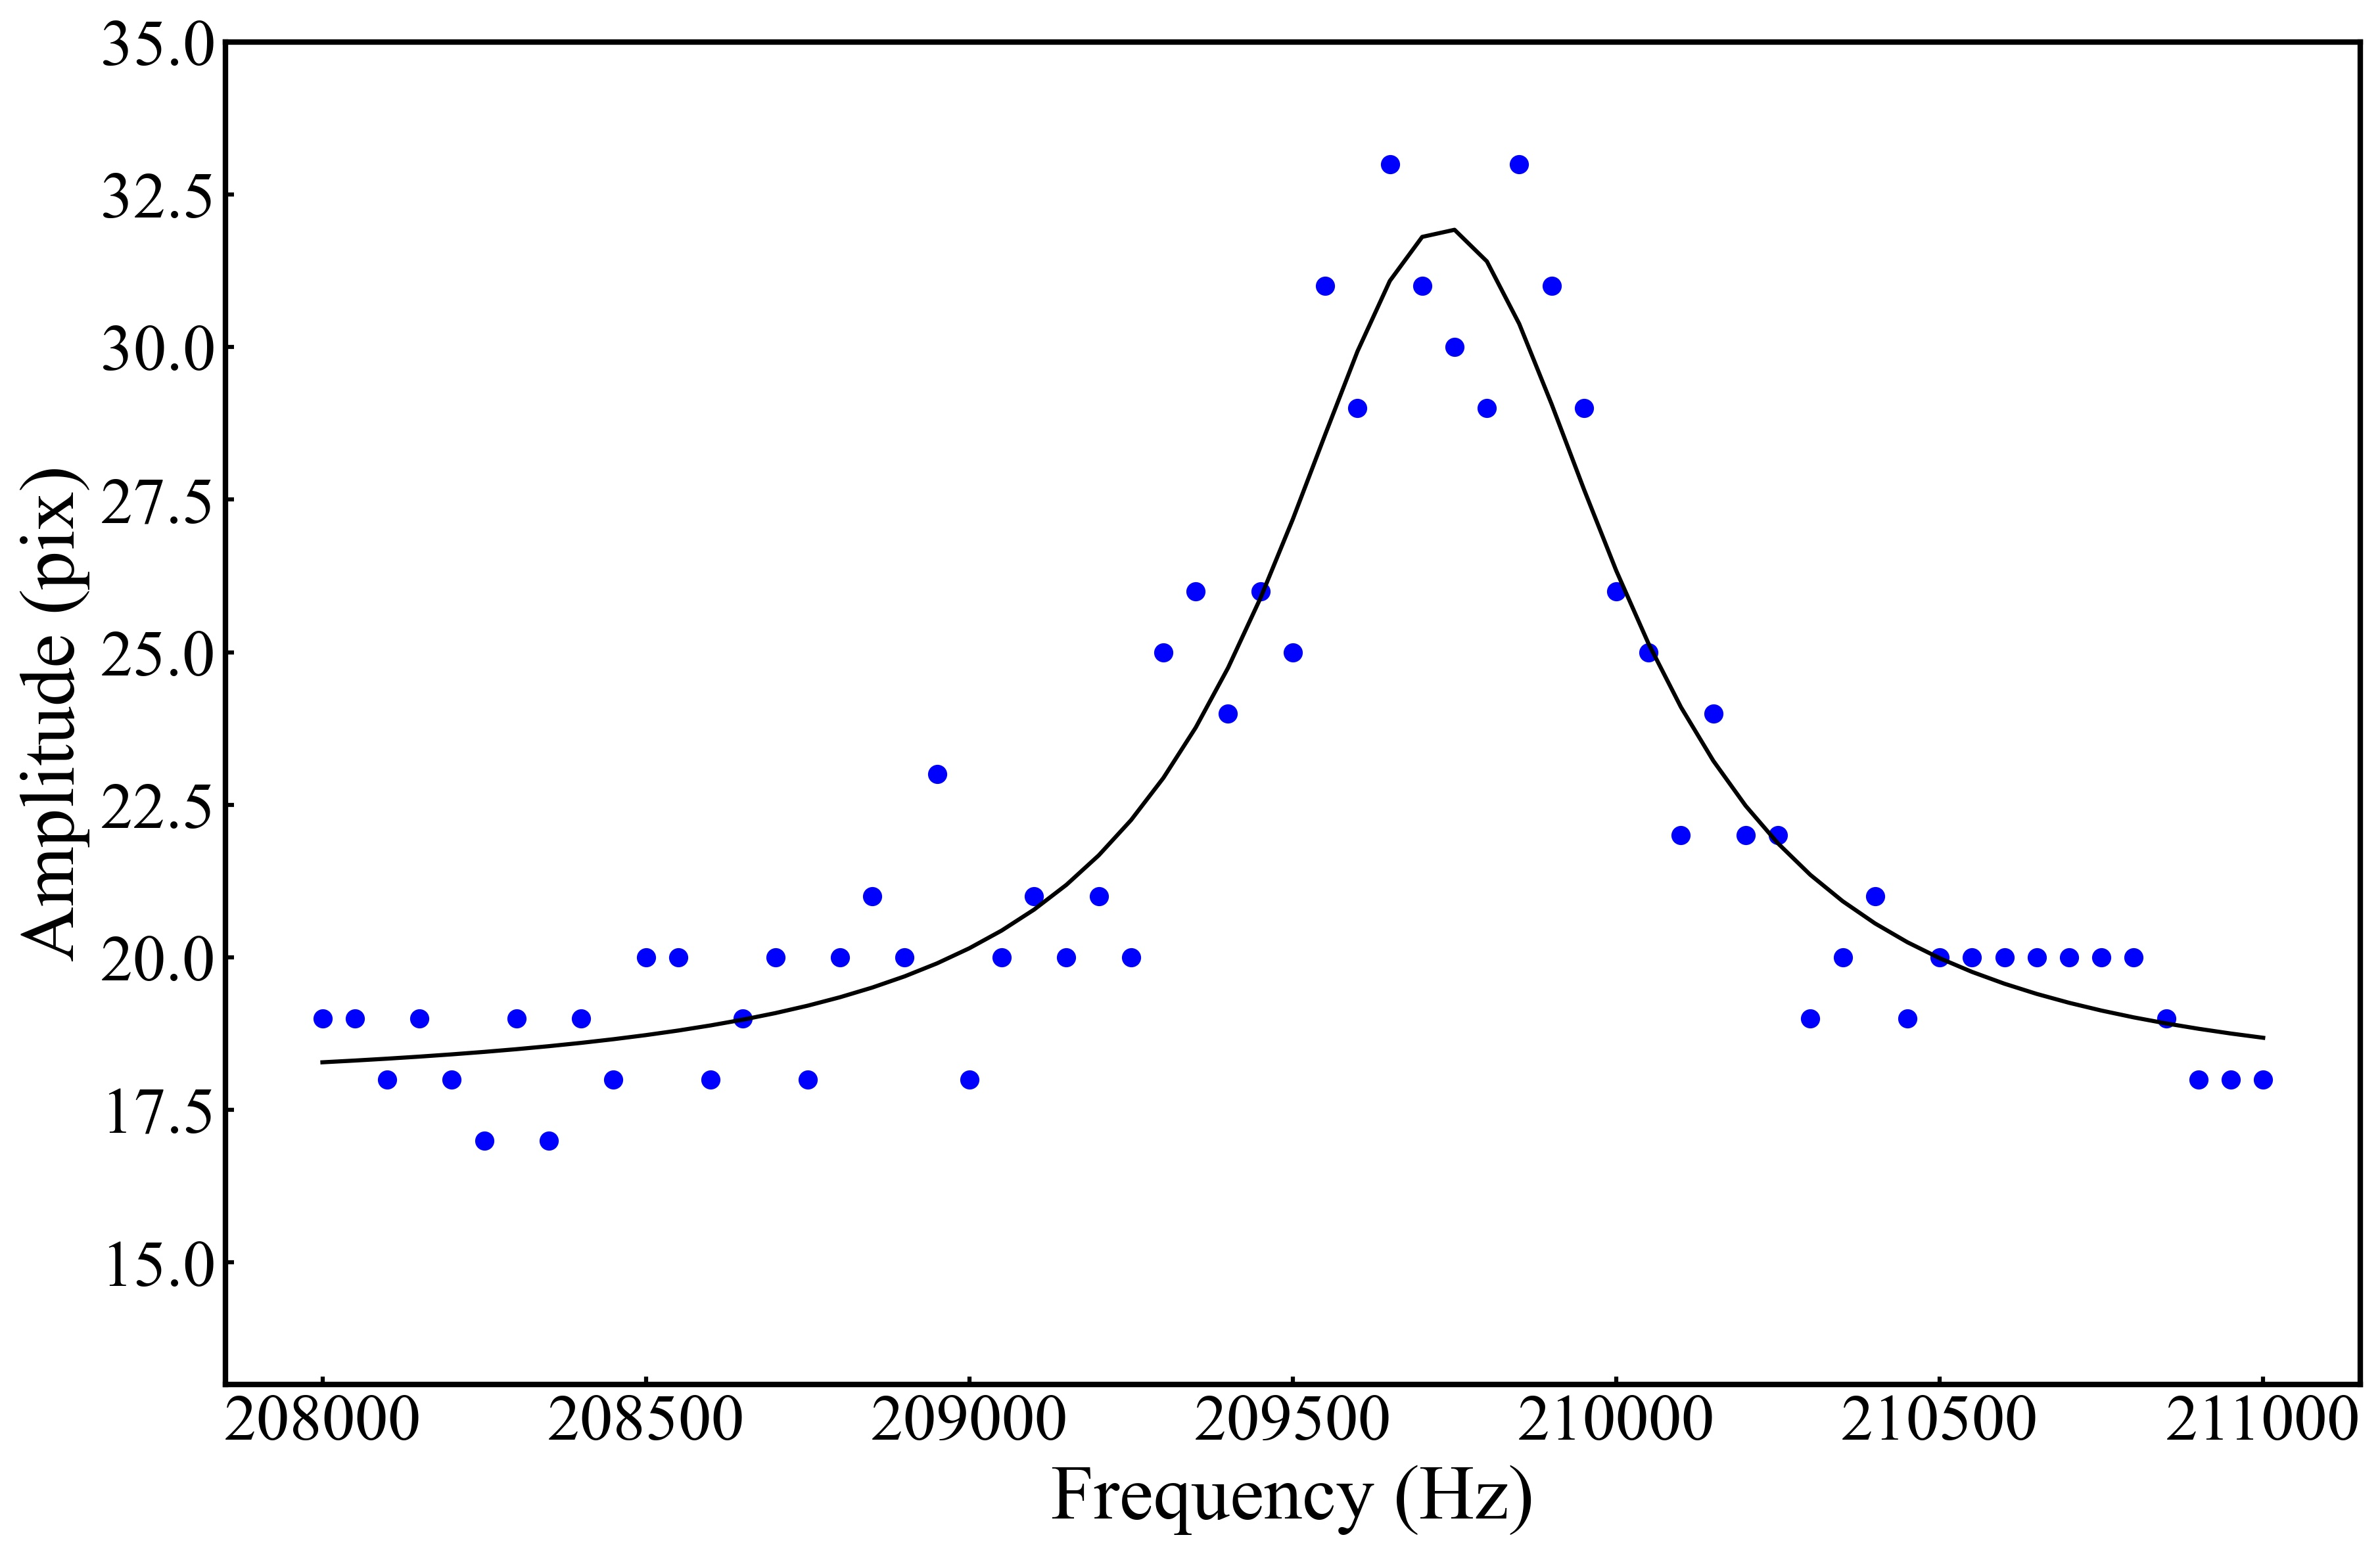
\includegraphics[width = 0.6\linewidth]{./methods/figure/fitting_result.jpg}
		\caption{\Tb{dc_string}のdc電圧セットに対するイオンの振幅の周波数特性とフィッティング結果}
		\label{fig:fitting_result}
\end{figure}

フィッティングパラメーターから,z方向の永年周波数は

\begin{align}
\frac{\omega_z}{2\pi} = 216.4 \pm 0.32 \  {\rm kHz} \notag
\end{align}

と決定される.なお,このときのac信号の振幅は200 mVppで周波数掃引は215 kHzから218 kHzまで50 Hz刻みで行った.

\clearpage

\section{イオン捕獲位置における電場の算出方法}

Python3.6の環境下で,NumPyとOpenCVのモジュールを利用して,イオン捕獲画像のヒストグラムの正規化と二値化およびイオンの位置特定を行った.カメラから得られるイオン捕獲画像を\Fig{raw_image}に示す.そして,イオンの位置特定の際の処理速度および精度の向上のため,ヒストグラムの処理をイオン捕獲位置の付近の範囲で行った(\Fig{rect_image}).

\begin{figure}[h]
	\begin{minipage}{0.48\linewidth}
		\begin{center}
			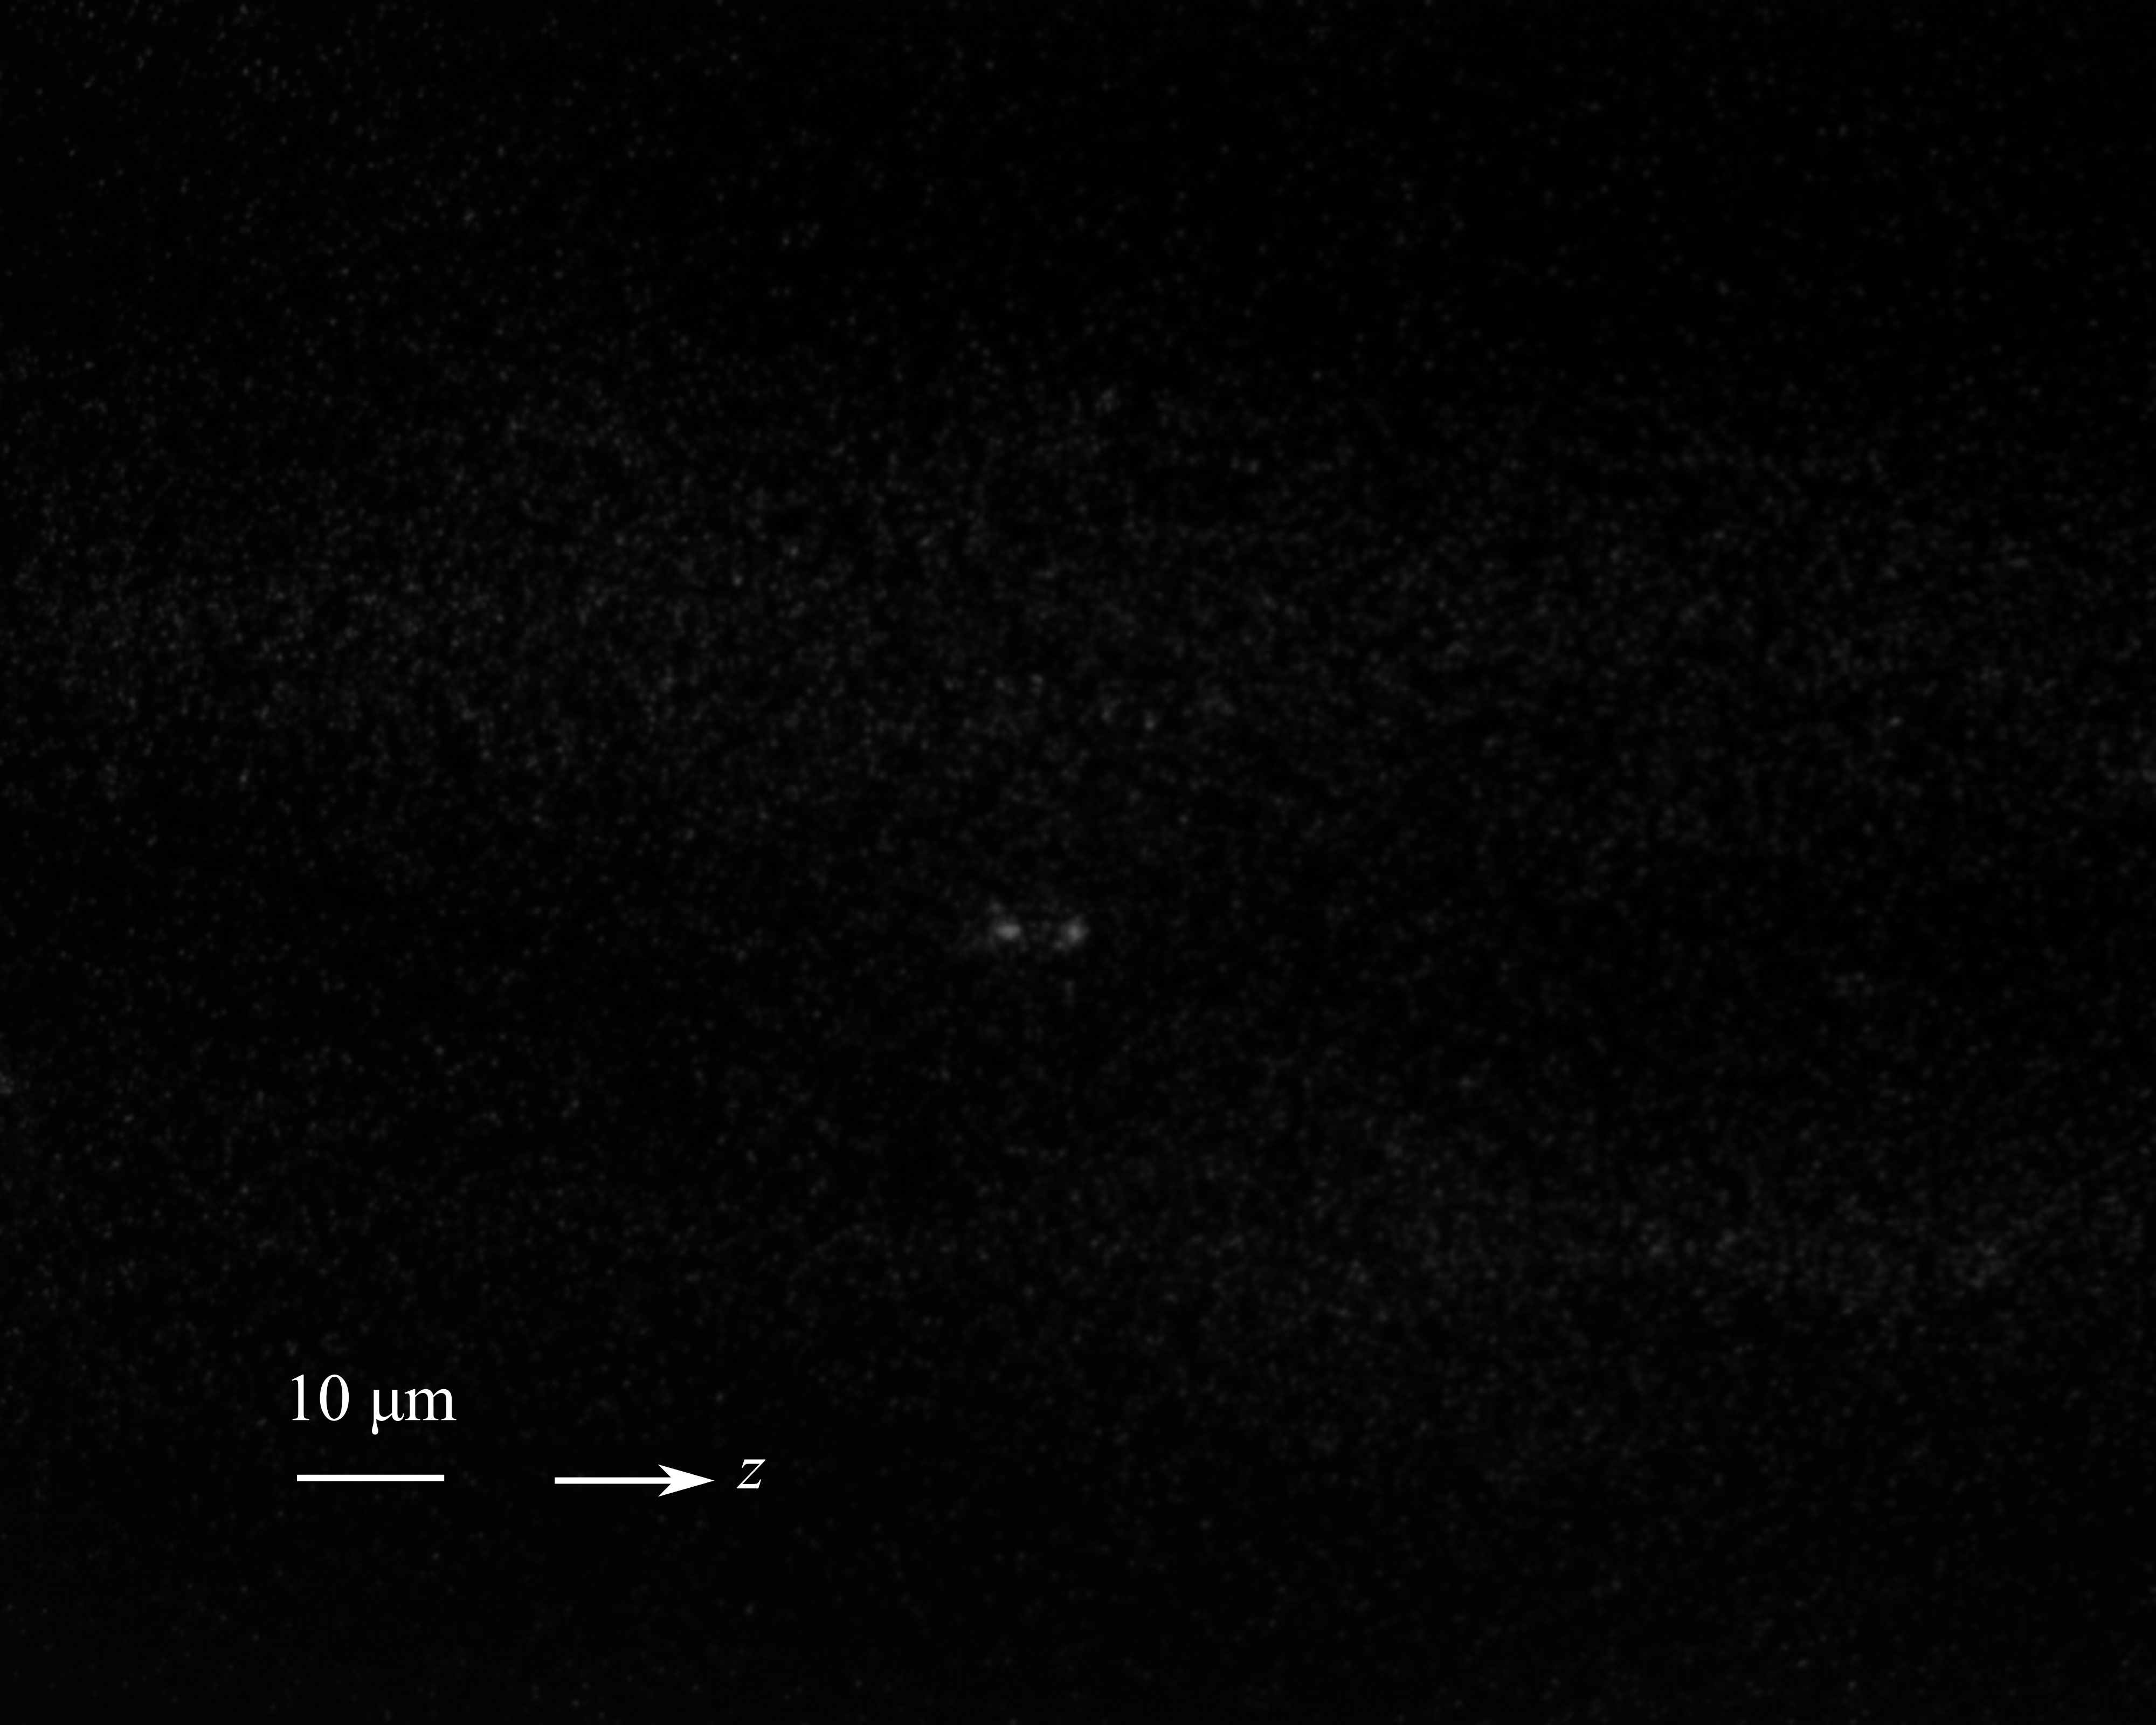
\includegraphics[width=0.6\columnwidth]{./methods/figure/raw_image.png}
			\caption{CCDカメラから得られるイオンの捕獲画像}
			\label{fig:raw_image}
		\end{center}
	\end{minipage}
	\begin{minipage}{0.48\linewidth}
		\begin{center}
			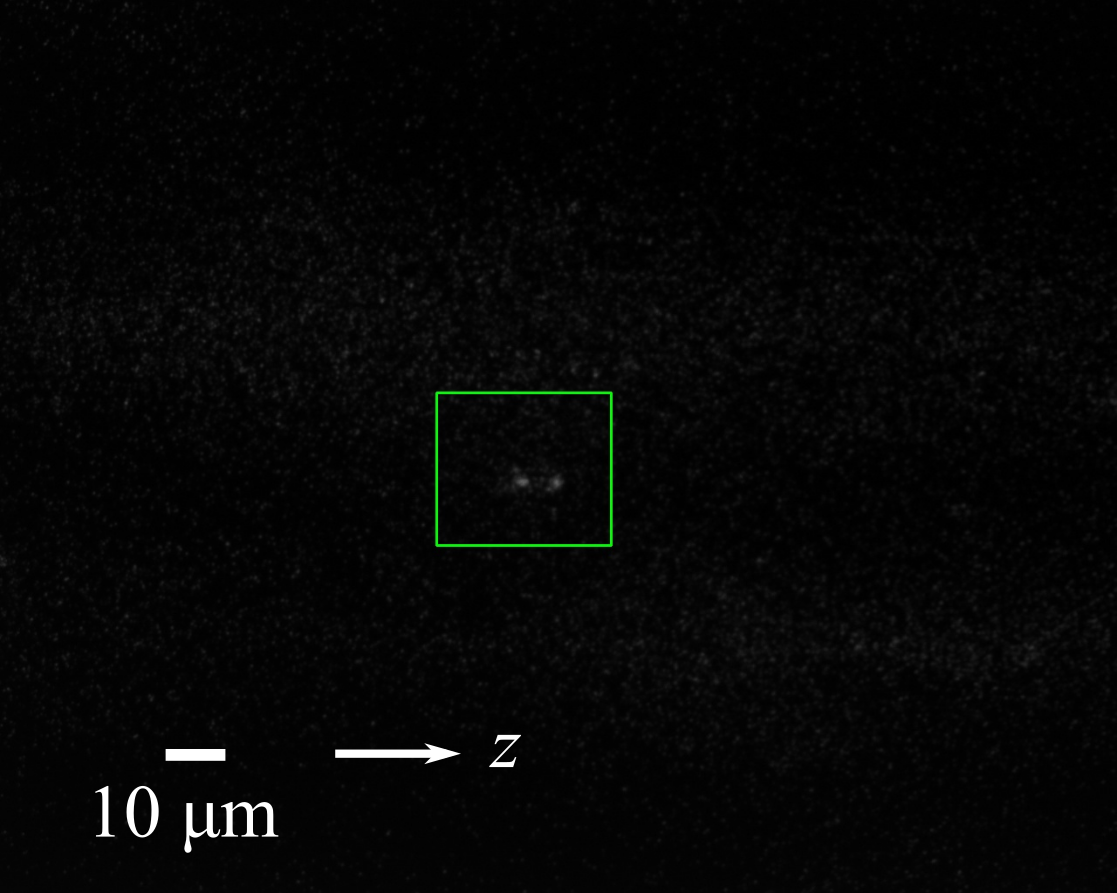
\includegraphics[width=0.6\columnwidth]{./methods/figure/rect_image.png}
			\caption{\Fig{raw_image}において画像処理を実行する範囲}
			\label{fig:rect_image}
		\end{center}
	\end{minipage}
\end{figure}

そして,得られたイオンの位置から平衡の式\Eq{equi_string}を用いてイオン捕獲位置における電場$\bm{E}(z_{i})$の算出を行った.

\begin{figure}[h]
	\begin{center}
		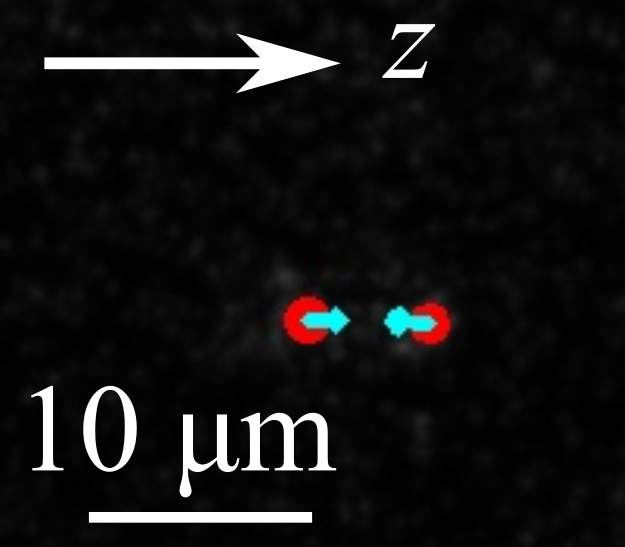
\includegraphics[scale=0.65]{./methods/figure/out_image.png}
		\caption{イオンの位置特定を行い,平衡の式\Eq{equi_string}を用いて算出した電場の大きさと向き(赤丸はイオンの位置を示し,青色の矢印の長さと向きは電場の大きさと向きを示している)}
		\label{fig:out_image}
	\end{center}
\end{figure}

\Fig{out_image}から算出された電場は,捕獲されたイオンのz座標を左から数えて$z_{1}, \ z_{2}$としたとき,

\begin{align*}
	E_{z}(z_1) &= 5.60 \ {\rm V/m} \\
	E_{z}(z_2) &= -5.60 \ {\rm V/m} 
\end{align*}

と計算される.使用したソースコードは\ref{source_code}に示している.